%!TEX root = these.tex

\chapter[Analyse de l'acquisition de cibles mobiles]{Analyse de l'acquisition de cibles mobiles}
\minitoc
\label{chap4}
\cleardoublepage

\section{Introduction}
	Dans ce chapitre nous présentons les résultats d'une étude empirique visant à caractériser les performances de sélection de cibles mobiles en fonction de la nature de leurs mouvements, dans un contexte aussi simple que possible : un ordinateur de bureau avec un écran monoscopique et une souris. Notre objectif étant de mieux comprendre cette tâche, dans le but éventuel d'aboutir à un modèle fiable, nous avons en effet cherché à limiter autant que possible l'influence de facteurs tels que la stéréoscopie (éventuellement adaptative), la nécessité de déplacements du corps entier, l'utilisation de périphériques peu familiers, etc. 
	
	Nous revenons premièrement sur le modèle de génération de mouvement introduit dans le chapitre~\ref{chap3}, ses capacités et limitations, et son extension 3D. Nous proposons d'autres extensions de ce modèle permettant de gérer les cas actuellement hors de sa portée.
	
	Nous étudions ensuite l'effet individuel des paramètres d'angle, de fréquence et de vitesse issus de notre modèle, puis les interactions entre ces effets. Nous relions ces paramètres et les conditions qu'ils engendrent aux impressions subjectives des participants à notre étude, afin d'établir quels facteurs perceptifs ou cognitifs influent sur les performances de sélection, selon la nature du mouvement des cibles.

	Dans ce but, nous examinons d'une part les profils de vitesse du curseur lors des tâches de sélection, en mesurant la durée relative de la phase balistique, et d'autre part le pouvoir prédictif des enveloppes convexes, introduites dans le chapitre~\ref{chap3}.
	
	Sur la base des enseignements que nous en tirons, nous proposons un guide pour la conception de techniques de sélection spécifiquement orientées vers les cibles mobiles, en précisant comment la nature des mouvements influe sur les contraintes imposées par la tâche, et sur les solutions possibles.

\section{Génération de mouvements}
	Si notre objectif est de caractériser les performances de sélection pour des cibles mobiles en fonction de la nature de leurs mouvements, notre intérêt se porte plus particulièrement sur les cibles de mouvements \og erratiques \fg{}, \og imprévisibles \fg{}, ou rappelant ceux d'une mouche.
	
	Ce focus a principalement deux motifs : premièrement, les chercheurs spécialisés dans la biologie structurale tentant d'utiliser des techniques de simulation de dynamique moléculaire interactive (voir le chapitre~\ref{chap1}) nous ont exprimé leurs difficultés d'interaction avec leurs systèmes, et particulièrement de sélection. Deuxièmement, de rapides tests empiriques suggéraient que les mouvements de ce type causaient les plus grandes difficultés pour des tâches de sélection.
	
	\subsection{Modèle VFA}
	Afin de tester cette hypothèse, nous avons conçu un modèle de génération de mouvements permettant, à l'aide d'un nombre de paramètres aussi petit que possible, de générer des mouvements aussi variés que possible dans leur nature. Pour rappel, il s'agit du modèle évoqué dans le chapitre~\ref{chap3}, et décrit par les paramètres suivants, pour définir le mouvement d'un objet de vecteur direction $\vec{dir}$ :
	
    \begin{enumerate}
    	\item La vitesse $V$ à laquelle l'objet se déplace ;
    	\item La fréquence $F$ des changements de $\vec{dir}$ ;
    	\item L'angle maximal $A$ de ces changements de direction : à chaque période $T = \frac{1}{F}$, $\vec{dir}$ subit une rotation d'un angle $\alpha$ échantillonné uniformément dans l'intervalle $[-A, +A]$.
    \end{enumerate}
    
    Du fait de son fondement sur les paramètres $V$, $F$ et $A$, nous appellerons simplement ce modèle $VFA$.
    
    \subsection{VFA en 3D}
    Quelques observations s'imposent. Tout d'abord, bien que décrit ici pour deux dimensions, ce modèle est naturellement extensible à l'espace tridimensionnel. En effet, les paramètres $V$, $F$ et $A$ ne changent pas ; seule un ajustement est nécessaire : la rotation du vecteur direction de l'objet animé doit se faire selon un axe qui, pour que la rotation effective soit toujours la même pour un angle donné, doit être orthogonal à $\vec{dir}$. Notre modèle étendu VFA3D fonctionne donc comme le modèle VFA, mais avec un axe de rotation orthogonal à $\vec{dir}$ choisi aléatoirement.
    
    \subsection{Un modèle puissant mais limité}
	Les capacités offertes par le modèle VFA sont très nombreuses, mais demeurent limitées, et ne peuvent couvrir tous les besoins possible en matière de génération de mouvement aléatoire.
    
    \subsubsection{Vitesse constante}
    Comme nous l'avons partiellement montré dans le chapitre~\ref{chap3}, le fait de varier les paramètres, en particulier $F$ et $A$, permet de générer des types de mouvement subjectivement très différents (voir les figures~\ref{fig:motion1530}, \ref{fig:motion4560}, \ref{fig:motion7590}, \ref{fig:motion105120}, \ref{fig:motion135150} et \ref{fig:motion165180}), et d'enveloppes convexes de tailles très différentes également (voir la figure~\ref{fig:trajAreas}). Néanmoins, et outre le problème des objets autocorrélés, notre modèle repose notamment sur une vitesse constante, ce qui, de fait, exclut tous les objets susceptibles d'accélérer. Là encore, ce choix fut fait pour limiter le nombre de paramètres, toujours dans l'objectif d'atteindre un compromis entre la simplicité du modèle et sa capacité à générer des mouvements que nos sujets puissent percevoir comme fondamentalement différents.
    
	Nous souhaitions tout particulièrement pouvoir générer du mouvement perçu comme \og régulier \fg{} ou \og prévisible \fg{} ainsi que du mouvement \og irrégulier \fg{}, \og saccadé \fg{} ou \og imprévisible \fg{}.
    
   	\subsubsection{Pas de véritable autocorrélation}
	Une autre obsevation très importante est que ce modèle ne peut générer que du mouvement markovien. En effet, à l'instant $t+1$, la rotation de $\vec{dir}$ générée est totalement indépendante de celle éventuellement générée à $t$, ou plus généralement de la dernière rotation générée, si elle existe. Cela ne signifie pas que $\vec{dir}_{t+1}$ soit indépendant de $\vec{dir}_{t}$, et il ne l'est pas, mais que le changement de direction à tout instant est indépendant du passé de l'objet concerné.
    
    Il en résulte que ce modèle ne peut générer du mouvement permettant d'étudier les performances de sélection sur des objets autocorrélés, tels que nous les avons définis et énumérés au cours du chapitre~\ref{chap3}. Ce choix reflète d'une part notre focus originel sur les simulations moléculaires (où il y a une demande claire émanant des utilisateurs) et d'autre part une volonté de conserver un modèle aussi simple que possible, afin de le rendre plus facile à utiliser, mais aussi pour pouvoir évaluer un échantillon représentatif des types de mouvements qu'il peut générer dans un laps de temps raisonnable pour une étude empirique, compte tenu notamment de la fatigue des sujets.
    
    \subsubsection{Mouvements pseudo-autocorrélés}
	Remarquons tout de même qu'une trajectoire générée par notre modèle peut, au moins temporairement, approximer un mouvement autocorrélé. Attendu qu'une tâche de sélection, pour peu qu'elle ne soit pas trop difficile, peut se dérouler sur une durée inférieure ou égale à la durée pendant laquelle le modèle VFA peut approximer un mouvement autocorrélé, il n'est pas nécessairement inutile pour étudier les performances de sélection de ces objets. On privilégiera dans ce cas de très fortes valeurs de $F$ et de très faibles valeurs de $A$. La figure~\ref{fig:autocorr} fournit deux exemples de telles trajectoires que nous proposons d'appeler pseudo-autocorrélées, générées avec $F \in \{30,120\}$ et $A \in \{1,2\}$.
	
	\begin{figure}[!htb]
		%\centering
		\begin{subfigure}[t]{0.49\textwidth}
			\centering
			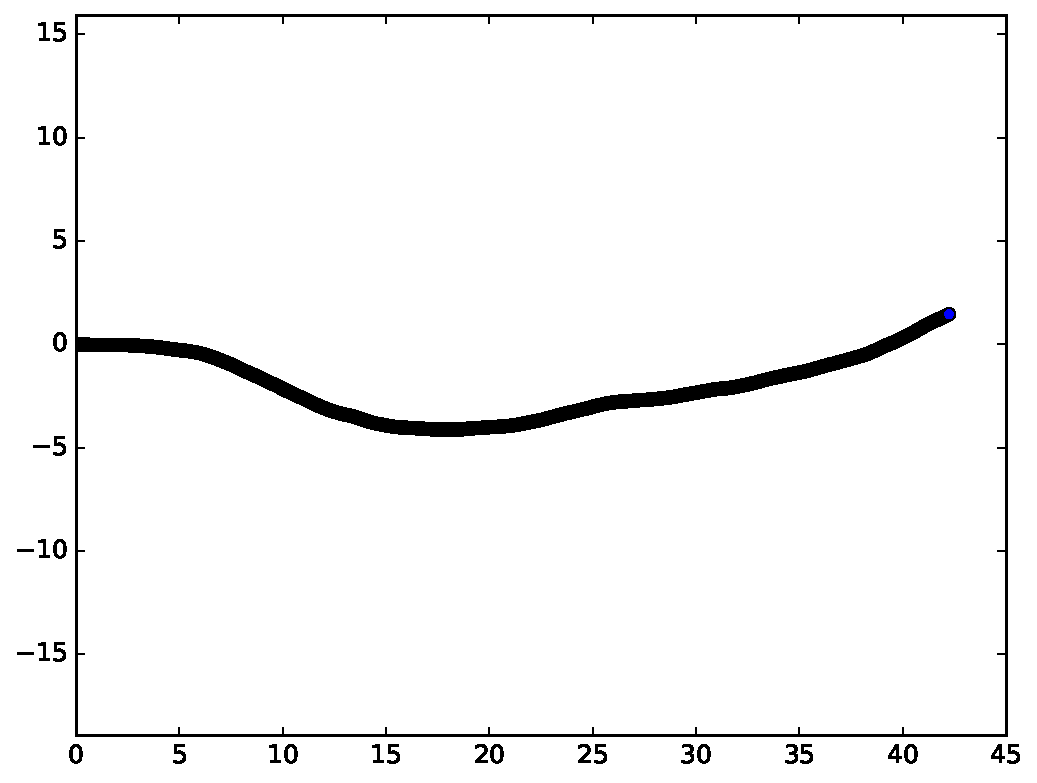
\includegraphics[width=\textwidth]{figures/ch4/ac_2_19_1_120a}
			\caption[Mouvement pseudo-autocorrélé A]{$F = 120$ et $A = 1$.}
			\label{fig:ac1_120A}
		\end{subfigure}
		~
		\begin{subfigure}[t]{0.49\textwidth}
			\centering
			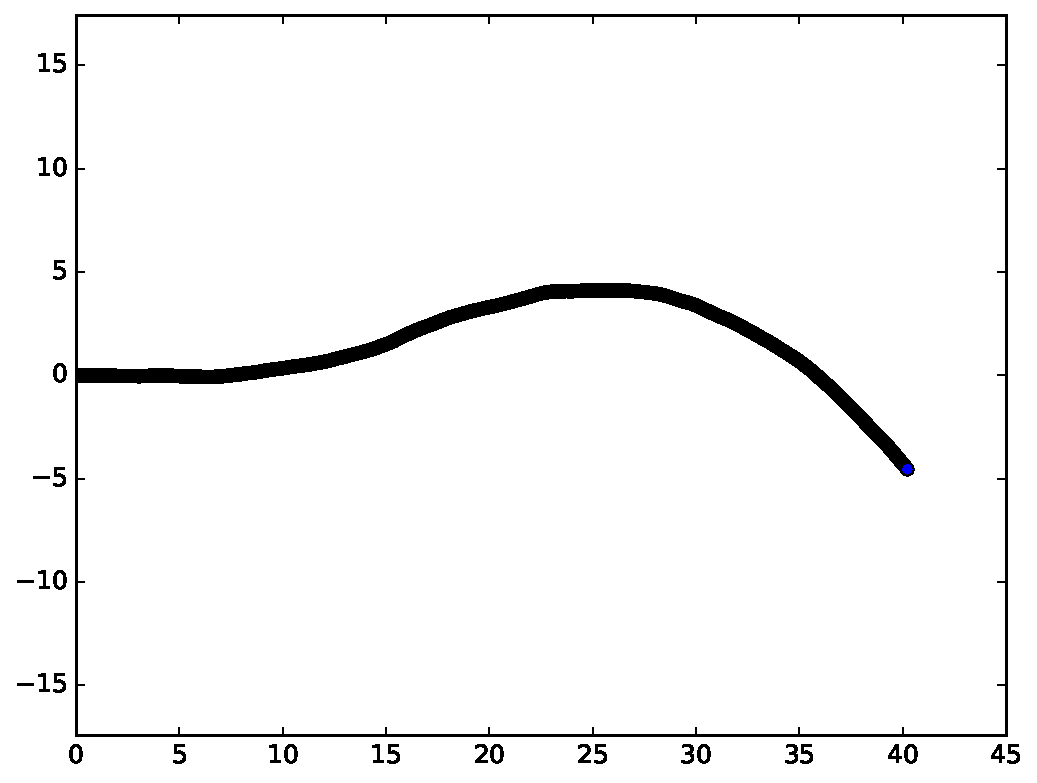
\includegraphics[width=\textwidth]{figures/ch4/ac_2_19_1_120b}
			\caption[Mouvement pseudo-autocorrélé B]{$F = 120$ et $A = 1$, bis.}
			\label{fig:ac_1_120B}
		\end{subfigure}
		~
		\begin{subfigure}[t]{0.49\textwidth}
			\centering
			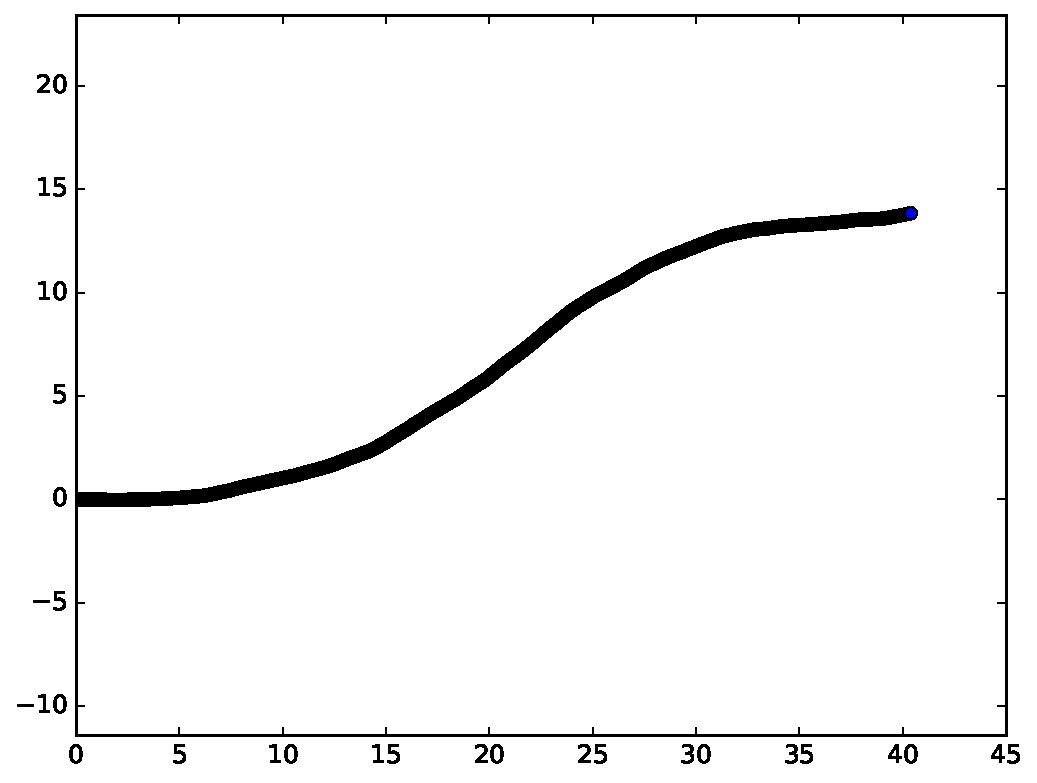
\includegraphics[width=\textwidth]{figures/ch4/ac_2_19_2_30}
			\caption[Mouvement pseudo-autocorrélé B]{$F = 30$ et $A = 2$.}
			\label{fig:ac_2_30}
		\end{subfigure}		
		~
		\begin{subfigure}[t]{0.49\textwidth}
			\centering
			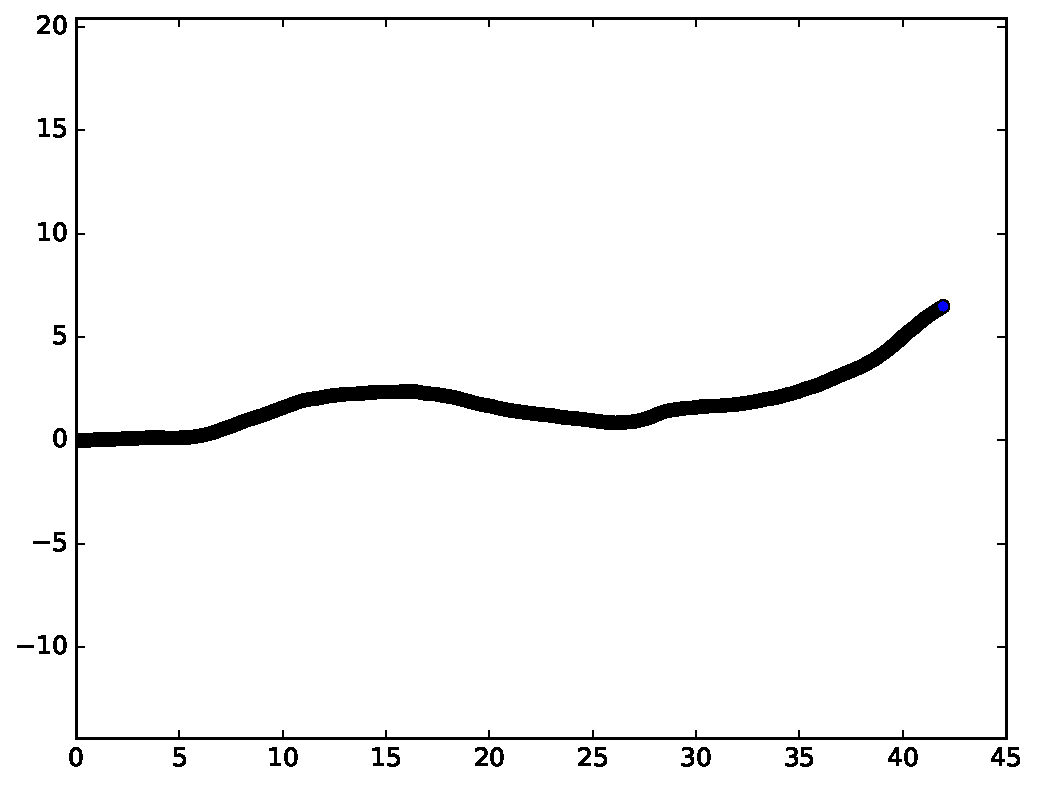
\includegraphics[width=\textwidth]{figures/ch4/ac_2_19_2_60}
			\caption[Mouvement pseudo-autocorrélé B]{$F = 120$ et $A = 1$, ter.}
			\label{fig:ac_1_120C}
		\end{subfigure}
		\caption[Mouvements pseudo-autocorrélés]{Trois trajectoires générées avec les mêmes valeurs $F = 120$~Hz et $A = 1\degree$, et une avec $F = 30$~Hz et $A = 2\degree$. Dans tous les cas, $V = 2,19$~cm/s. Ces trajectoires ressemblent à celles que l'on pourrait attendre d'objets autocorrélés, tels que des véhicules, par exemple.}
		\label{fig:autocorr}
	\end{figure}
    
    \subsection{Proposition de modèles de génération de mouvements autocorrélés}
    Les objets autocorrélés présentent néanmoins un intérêt certain, et les trajectoires pseudo-autocorrélées ne sont que des approximations qui peuvent s'avérer unsuffisantes. Ces objets pourraient faire l'objet d'études spécifiques pour lequelles de telles approximations ne seraient pas suffisantes. Nous proposons donc ici deux modèles différents permettant de générer des mouvements réellement autocorrélés.
    
    \subsubsection{Modèle VFA à mémoire}
    Une première option pour un modèle adapté aux objets autocorrélés serait d'adapter le modèle VFA en lui ajoutant une mémoire, par exemple une mémoire du dernier changement de direction de l'objet concerné. L'on retiendrait ainsi l'angle du changement de direction à l'instant précédent ($\alpha_{t-T}$, avec $T = \frac{1}{F}$), et l'on pourrait appliquer un nouveau changement avec un angle plus ou moins proche de ce dernier, selon des paramètres. L'équation~\ref{eq:vfamem} présente une possibilité, où $\alpha$ est échantilloné entre $-A$ et $+A$, et $c_{ac} \in [0,1]$ est un coefficient d'autocorrélation.
    
    \begin{equation}
		\alpha_{t} = \alpha_{t-T} \times c_{ac} + \alpha (1 - c_{ac})
		\label{eq:vfamem}
    \end{equation}
    
	Ainsi, lorsque le coefficient d'autocorrélation est nul, le système devient markovien ; lorsqu'il vaut 1, $\alpha_{nT}$ est constant (avec $n \in \mathbb{N}$). De fait, s'il est non nul, l'objet aura un mouvement circulaire s'il est ciné-continu et régulier s'il est ciné-discret ; s'il est nul, le mouvement sera rectiligne dans les deux cas.
    
    \subsubsection{Modèle newtonien}
    Une seconde option ayant le mérite d'avoir un certain sens physique consisterait à considérer chaque objet comme une particule dotée d'une masse, et de la soumettre à une force qui, elle, serait régie par un modèle de type VFA, éventuellement modifié pour remplacer la vitesse par la norme de la force, notamment. Sans doute serait-il également opportun d'appliquer une force de friction afin d'éviter que l'application (même approximativement) constante d'une force (et donc d'une accélération\footnotemark{}) ne mène à des vitesses potentiellement croissantes et non bornées.
    
    \footnotetext{Rappelons que, d'après la seconde loi de Newton~\cite{newton1833philosophiae}, $\vec{F} = m\vec{a}$ où $F$ est une force, $m$ est la masse de l'objet sur lequel elle agit, et $\vec{a}$ est l'accélération de l'objet, soit $\vec{a} = \frac{\vec{F}}{m}$, où l'on voit bien que l'application d'une force constante à un objet de masse constante mène à une accélération constante, donc à une vitesse croissant linéairement. En l'absence de résistance à $\vec{F}$, la vitesse n'est pas bornée.}
    
    Le modèle nécessiterait un calibrage précis pour obtenir le comportement souhaité, notamment en ce qui concerne les masses des objets ou le coefficient de friction. Notons par ailleurs que, sauf dans certains cas particuliers (et après une période dynamique) les vitesses des objets ne seraient pas constantes pour une norme de $\vec{F}$ donnée, ce qui distinguerait ce modèle newtonien du nôtre (VFA). En soi, ce n'est pas nécessairement un problème --- et peut même être un avantage --- mais cela complique le contrôle des propriétés d'un environnement synthétique créé pour mener une étude empirique.

\section{Expérience et protocole}
	Nous avons mené une étude empirique visant à évaluer les performances de sélection de cibles mobiles en fonction de la nature du mouvement. Nous avions 13 sujets, âgés de 14 à 56 ans. Ils avaient pour tâche de cliquer sur une cible mobile (un disque) affichée sur un écran d'ordinateur de bureau.

	\subsection{Dispositif expérimental}
	Le périphérique de saisie était une souris standard sans accélération, afin d'éviter le biais potentiel introduit par une fonction de gain pouvant être familière pour certains utilisateurs et pas pour d'autres. Cette souris pilotait un curseur cruciforme gris. Le moniteur était un Dell \emph{UltraSharp U2412M}\footnotemark{}, de 24 pouces (60,96~cm) de diagonale, et d'environ 94 pixels par pouce (37 pixels par cm).
	
	La tâche elle-même était toutefois limitée à une fenêtre carrée de 1000 pixels de côté, soit 26,92~cm.

	\footnotetext{\url{http://www.dell.com/en-us/work/shop/cty/pdp/spd/dell-u2412m}}

	\subsection{Tâche et conditions}
	\subsubsection{Description de la tâche}
	La tâche consistait à sélectionner une cible parmi 50 objets identiques : des disques de 5,4~mm de diamètre. Les 49 \og distracteurs \fg{} étaient affichés en gris, et la cible à sélectionner était rouge, comme l'illustre la figure~\ref{fig:app}. Les distracteurs et la cible étaient mus selon les mêmes paramètres V, F et A de notre modèle, mais l'angle $\alpha$ échantillonné à chaque période T était échantillonné séparément pour chaque objet, donc généralement différent. Lorsqu'un disque \og percutait \fg{} le bord de la fenêtre, il \og rebondissait \fg{} dessus.
	
	\begin{figure}[!htb]
		\centering
		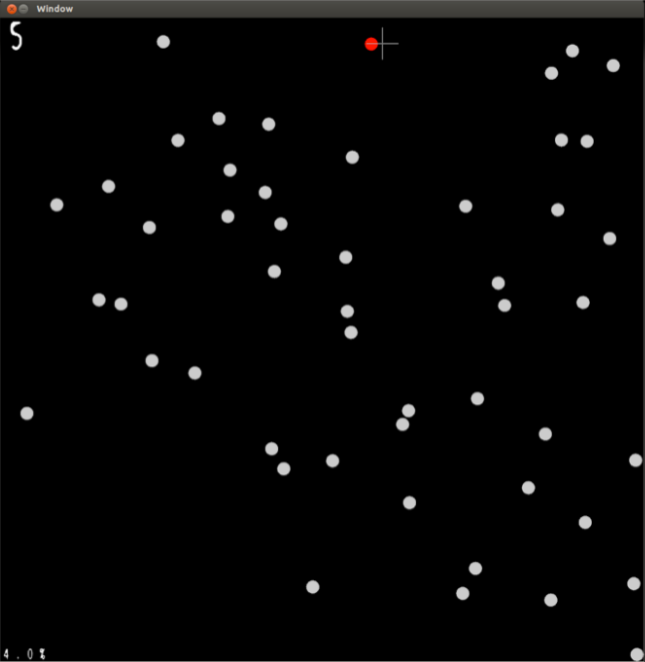
\includegraphics[width=\textwidth]{figures/ch4/app}
		\caption[Application utilisée dans notre évaluation]{Application utilisée dans notre évaluation. Le curseur gris s'approche de la cible rouge (qui n'est pas sélectionnable ici, car le centre du curseur cruciforme n'est pas inclus dans le disque) et les distracteurs gris se déplacent dans la fenêtre. Le nombre de tentatives de sélection encore possibles pour la cible courante est affiché en haut à gauche --- 5 dans le cas présent. Le taux de complétion de l'expérience dans son ensemble est inscrit en bas à gauche.}
		\label{fig:app}
	\end{figure}
	
	Ce choix, qui altère ponctuellement le mouvement généré par le modèle VFA, fut fait pour d'une part éviter la disparition d'une cible hors de la fenêtre, pour éviter toute discontinuité (par exemple si la cible réapparaissait de l'autre côté de la fenêtre), et pour limiter la \og surprise \fg{} éprouvée par l'utilisateur en imitant un phénomène physique familier. Cela permet par ailleurs de garantir la constance la densité de l'environnement.
	
	Pour contrôler l'amplitude (telle que définie par Fitts~\cite{fitts1954information}) les mouvements des distracteurs étaient légèrement contraints, de telle sorte qu'après la sélection d'une cible, la distance entre le curseur et la cible suivante était à peu près constante (environ 7,96~cm).
	
	Quand une cible était sélectionnée avec succès, elle changeait brièvement de couleur pour devenir verte tandis que la cible suivante devenait rouge.
	
	\subsubsection{Erreurs et échecs}
	La sélection de cibles implique un compromis entre vitesse et précision~\cite{guiard2011fitt}, et les utilisateurs sont généralement libres d'adopter différentes approches de ce compromis, privilégiant le premier ou le second objectif. Il peut en résulter, d'un utilisateur à l'autre, d'importants écarts de temps de sélection et de taux d'erreurs. Afin de minimiser ces variations, nos sujets avaient pour instruction de sélectionner leurs cibles le plus rapidement possible, mais avec un maximum de 5 tentatives.
	
	Le nombre de tentatives encore possible était affiché dans le coin supérieur gauche de la fenêtre (voir la figure~\ref{fig:app}). Après la dernière tentative, en cas d'échec le mot \emph{failure} était affiché à la place du nombre de tentatives, indiquant un échec. Mais les sujets avaient pour instruction de continuer à essayer de sélectionner la cible, sans plus chercher à minimiser les erreurs. Cette particularité de notre dispositif expérimental était nécessaire pour avoir suffisamment de données (en temps de sélection) pour les conditions les plus difficiles, qui généraient énormément d'erreurs.
	
	Elle a néanmoins l'inconvénient de réduire quelque peu les temps de sélection des conditions les plus difficiles, tout en augmentant leurs taux d'erreurs. Ainsi, les échecs ne sont pas absolus, mais indiquent les conditions pour lesquelles la sélection est (parfois extrêmement) difficile.
	
	\subsubsection{Conditions évaluées}
	Nous avons testé toutes les combinaisons des valeurs de V, F et A suivantes, avec 4 sélections par condition et par sujet :
	
	\begin{description}
		\item[V :] 0,73, 1,46 et 2,19~cm/s, soit 3 valeurs ;
		\item[F :] 1, 2, 4, 8, 13, 20 et 30~Hz, soit 7 valeurs ;
		\item[A :] 0, 30, 60, 90, 120 et 180 degrés, soit 6 valeurs.
	\end{description}
	
	À ceci s'ajoutait une condition de base avec des cibles statiques, répétée 20 fois. Naturellement, lorsque $A = 0$, les cibles se déplacent en ligne droite. Au total, nous avons évalué $3 \times 7 \times 6 + 1 = 127$ conditions ave 4 essais par condition dynamique et 20 essais pour la condition statique, soit un total de $126 \times 4 + 1 \times 120 = 524$ essais par participant, et $524 \times 13 = 6812$ essais au total.
	
	La conception de ce protocole impliquait un compromis difficile entre plusieurs objectifs contradictoires : avoir suffisamment de conditions pour évaluer un échantillon représentatif des types de mouvements possibles, avoir suffisamment de données par condition pour avoir des résultats fiables, limiter l'évaluation dans le temps et dans l'intensité pour limiter la fatigue des sujets et ne pas les décourager.
	
	\paragraph{Choix des valeurs évaluées.}
	Les valeurs de V (dont la deuxième est le double de la première, et la troisième le triple) furent choisies pour avoir une vitesse faible générant des sélections faciles, une vitesse intermédiaire, et une vitesse élevée générant des conditions difficiles.
	
	Les valeurs de F furent choisies pour couvrir l'espace des fréquences qu'un utilisateur peut percevoir comme significativement différentes. Nous avons en effet observé au cours de plusieurs études pilotes que l'augmentation de la fréquence au-delà de 30~Hz n'était pas très sensible, mais que de petites différences absolues pouvaient être significatives si elles étaient relativement grandes ; par exemple, passer de 1~Hz à 2~Hz revient à n'ajouter qu'un seul hertz, mais à doubler la fréquence. Il était donc nécessaire d'avoir une plus forte densité de valeurs testées dans les basses fréquences que dans les hautes.
	
	Les valeurs de A résultent d'un constat similaire, mais moins marqué. Ainsi, les valeurs évaluées vont simplement de 0\textdegree{} à 180\textdegree{} par pas de 30\textdegree{} ; la valeur 150\textdegree{} est omise car trop similaire (subjectivement) aux valeurs 120\textdegree{} et 180\textdegree{}, et afin de limiter le nombre de conditions.

	\subsection{Procédure et collecte de données}
	\subsubsection{Descrption de la procédure}
	Chaque session durait environ 40 minutes (selon les performances du sujet) dont une phase d'entraînement de plus de 50 essais, prenant fin au moment où le sujet se sentait suffisamment à l'aise pour commencer l'évaluation.
	
	Des pauses d'une durée laissée au choix du sujet étaient accordées à 25~\%{}, 50~\%{} et 75~\%{} de complétion de l'évaluation, afin de limiter les effets de la fatigue. Permettons-nous en effet d'insister sur le fait que la tâche nécessite une concentration intense et soutenue, en plus d'un effort physique non négligeable compte tenu de la rapidité et de la précision requises. Les pauses étaient donc généralement appréciées.
	
	À la fin de l'évaluation, un court questionnaire était soumis aux sujets afin de recueillir leurs impressions subjectives sur les différentes \og classes \fg{} de mouvements qu'ils étaient capables d'identifier, et les éventuelles stratégies qu'ils avaient pu mettre en place pour chaque classe.
	
	\subsubsection{Données collectées}
	Pour chaque essai, nous avons mesuré :
	
	\begin{description}
		\item[Le temps de sélection :] entre l'instant où la cible devient rouge et celui où elle est effectivement sélectionnée,
		\item[Les erreurs :] le nombre de clics hors de la cible,
		\item[Les échecs :] lorsqu'une tâche engendre au moins cinq erreurs,
		\item[La position de la cible] tout au long de la tâche,
		\item[La position du curseur,] également tout au long de la tâche.
	\end{description}

\section{Résultats : performances de sélection}
	Les valeurs présentées ici sont des moyennes calculées sur l'ensemble de nos sujets.
	
	\subsection{Temps de sélection}
	Les performances de sélection dans les conditions les plus faciles étaient relativement stable d'un sujet à l'autre : le plus lent fut moins de quatre fois plus lent que le plus rapide pour le mouvement rectiligne. Cependant, pour les conditions les plus difficiles, les écarts peuvent être considérables, d'un facteur supérieur à 18 du sujet le plus rapide au plus lent.
	
	\subsubsection{Temps de sélection normalisés}
	Par conséquent, et pour éviter d'accorder trop de poids aux sujets les plus lents, nous avons choisi de normaliser les temps de sélection par sujet. Ainsi, pour chaque sujet, le temps de sélection normalisé (TSN) est la moyenne des temps de sélection par condition, normalisée selon la condition la plus difficile \emph{pour le sujet en question}.
	
	Par exemple, si une condition a un TSN de 0,75 pour un sujet donné, cela signifie qu'il a fallu à ce sujet (en moyenne sur les 4 essais) 75~\%{} du temps dont il a eu besoin (en moyenne sur les 4 essais) pour la condition qui lui a demandé le plus de temps. La moyenne des temps de sélection normalisés (MTSN) d'une condition est donc la moyenne des TSN de tous les sujets pour cette condition.
	
	Attendu que la condition la plus difficile n'est pas nécessairement la même pour tous les sujets, aucune condition n'a une MTSN de 1,0.
	
	\subsection{Erreurs et échecs}
	\subsubsection{Erreurs}
	Le nombre d'erreurs est compris entre 0 et 5 (les clics erronés ne sont pas comptabilisés après le cinquième, attendu que les sujets ont dans ce cas pour instruction de ne pas chercher à éviter les erreurs --- ils sont toutefois enregistrés). Un taux d'erreur (TERR) de 3,5 pour une condition donnée signifie donc qu'en moyenne, les sujets ont fait 3,5 clics hors de la cible pour ladite condition.
	
	\subsubsection{Échecs}
	Un échec survient lorsque pour une tâche de sélection, un sujet commet au moins 5 erreurs. 	Un taux d'échecs (TECH) de 50~\%{} pour une condition donnée signifie que la moitié des essais pour cette condition ont mené à un échec (5 clics erronés ou plus) sur l'ensemble des sujets.
	
	Notez que du fait d'inquiétudes croissantes dans divers domaines de recherche concernant les limites des tests de significativité d'hypothèse nulle~\cite{dragicevic2014running, cumming2014new}, nos analyses se fondent principalement sur les tailles d'effets, rapportés ici sous forme de différences de pourcentage $p$, calculées selon la formule suivante, pour deux mesures $m_{1}$ et $m_{2}$ : $p = 100 \times \frac{\abs*{m_{2} - m_{1}}}{\frac{m_{1} + m_{2}}{2}}$.

	\subsection{Vitesse}
	Sans surprise, les temps de sélection et les taux d'erreurs croissent avec la vitesse des cibles, comme l'illustre la figure~\ref{fig:spEffectPerf}. Ainsi, la moyenne des MTSN de toutes les conditions lentes (0,73~cm/s) est de 16,74~\%{}, celle des conditions de vitesse intermédiaire est de 25,02~\%{}, et celle des conditions rapides est de 36,58~\%{}. Les différences de pourcentages croisées entre ces conditions sont présentées dans le tableau~\ref{tab:spPerf}.

	Les MTSN, TERR et TECH en fonction de la vitesse sont présentés sur la figure~\ref{fig:spEffectPerf}, pour des valeurs de A de 60 et 120, et pour toutes les valeurs de F. Les conditions associées aux autres valeurs de A sont omises ici, dans un souci de concision, mais présentent des caractéristiques très similaires.
	
%	\newcommand{\newrow}{\bigstrut[t] \\ \hline}
	\begin{table}
		\centering
		\begin{tabular}{r c | c c c}
			Vitesse			&			& Basse		& Moyenne	& Haute		\bigstrut[b] \\
							&			& (16,74)	& (25,02)	& (36,58)	\bigstrut[b] \\ \hline
			Basse			& (16,74)	& 0,00		& 39,65		& 74,40		\bigstrut[t] \\
			Moyenne			& (25,02)	& 39,65		& 0,00		& 37,51		\\
			Haute			& (36,58)	& 74,40		& 37,51		& 0,00		\\
		\end{tabular}
		\caption[Performances selon la vitesse]{Performances de sélection (MTSN moyennes) selon la vitesse, et différences de pourcentages. Les MTSN moyennes associées à chaque vitesse sont présentées sur la première ligne et la première colonne en pourcentages, et les différences de pourcentages croisées sont indiquées à l'intérieur du tableau.}
		\label{tab:spPerf}
	\end{table}
	
	On observe que les MTSN et TERR sont approximativement des fonctions affine de la vitesse, pour une pseudo-entropie (i.e., le produit AF) donnée. Les TECH tendent à croître de façon super-linéaire, probablement du fait de l'effet de seuil introduit par notre définition (arbitraire) d'un échec.

	\newcommand{\subImgWlineplot}{0.48\textwidth}
	\begin{figure}[!htb]
		\centering
		\begin{subfigure}[t]{\subImgWlineplot}
			\centering
			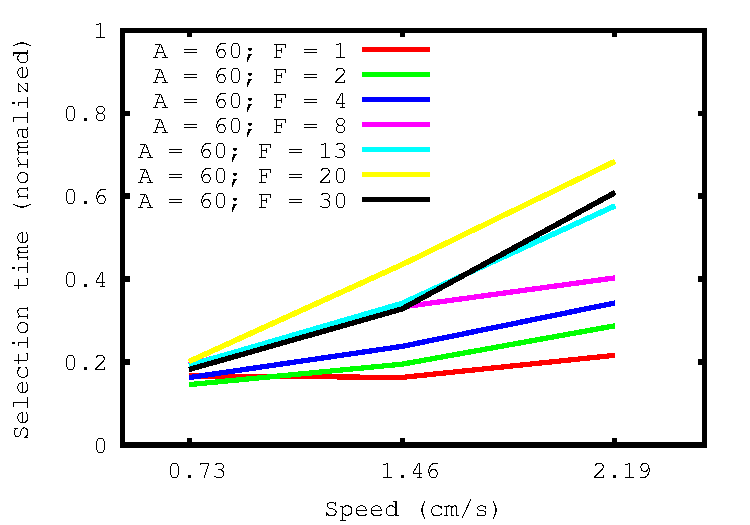
\includegraphics[width=\textwidth]{figures/ch4/speed_angle_60_times}
			\caption{MTSN pour $A = 60$.}
			\label{fig:spEffect_t_60}
		\end{subfigure}
		~
		\begin{subfigure}[t]{\subImgWlineplot}
			\centering
			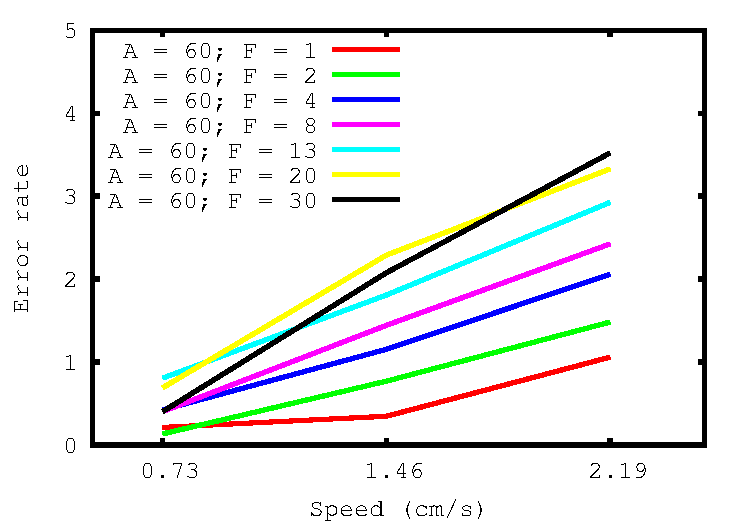
\includegraphics[width=\textwidth]{figures/ch4/speed_angle_60_errors}
			\caption{Taux d'erreurs pour $A = 60$.}
			\label{fig:spEffect_e_60}
		\end{subfigure}
		~
		\begin{subfigure}[t]{\subImgWlineplot}
			\centering
			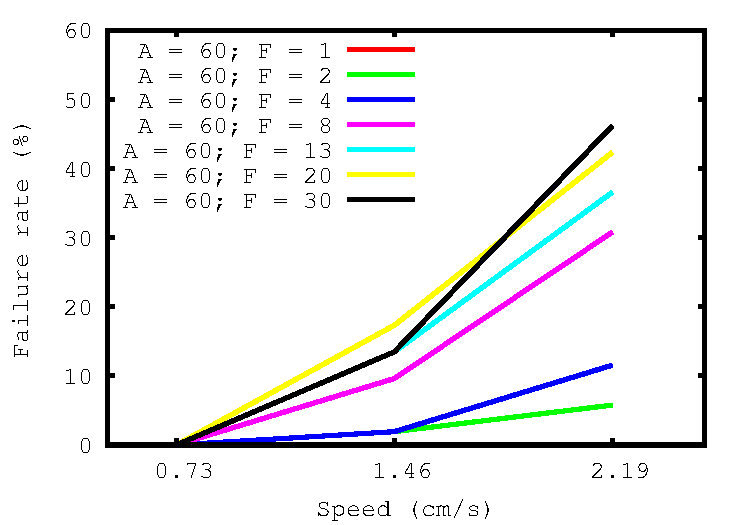
\includegraphics[width=\textwidth]{figures/ch4/speed_angle_60_failures}
			\caption{Taux d'échecs pour $A = 60$.}
			\label{fig:spEffect_f_60}
		\end{subfigure}
		~
		\begin{subfigure}[t]{\subImgWlineplot}
			\centering
			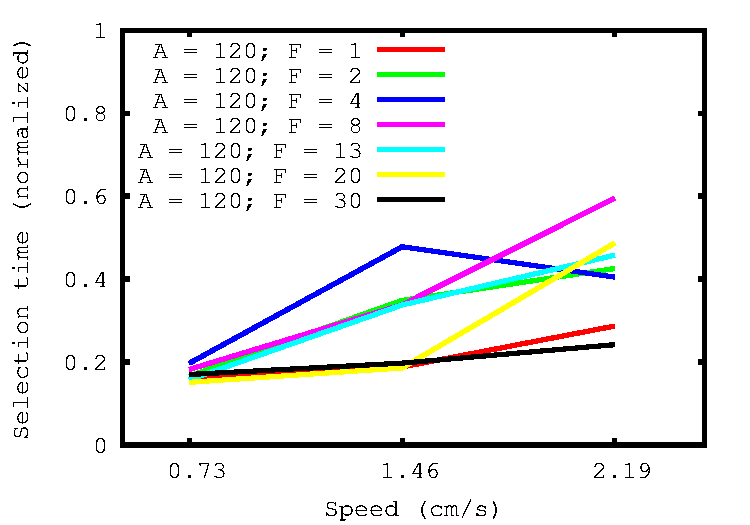
\includegraphics[width=\textwidth]{figures/ch4/speed_angle_120_times}
			\caption{MTSN pour $A = 120$.}
			\label{fig:spEffect_t_120}
		\end{subfigure}
		~
		\begin{subfigure}[t]{\subImgWlineplot}
			\centering
			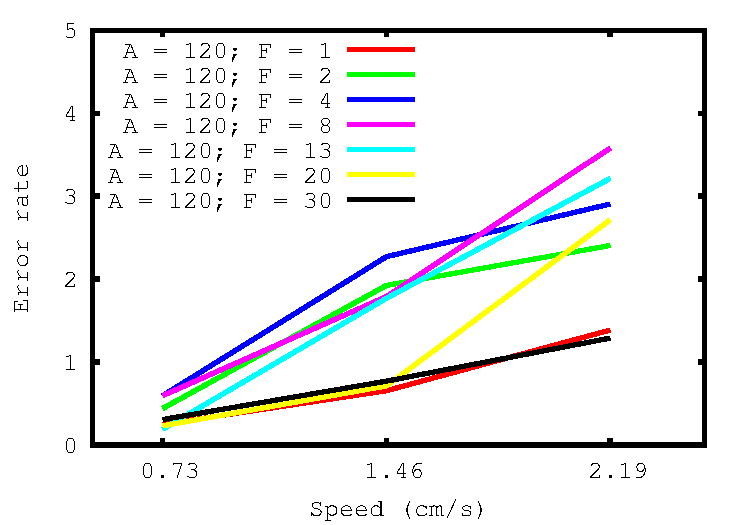
\includegraphics[width=\textwidth]{figures/ch4/speed_angle_120_errors}
			\caption{Taux d'erreurs pour $A = 120$.}
			\label{fig:spEffect_e_120}
		\end{subfigure}
		~
		\begin{subfigure}[t]{\subImgWlineplot}
			\centering
			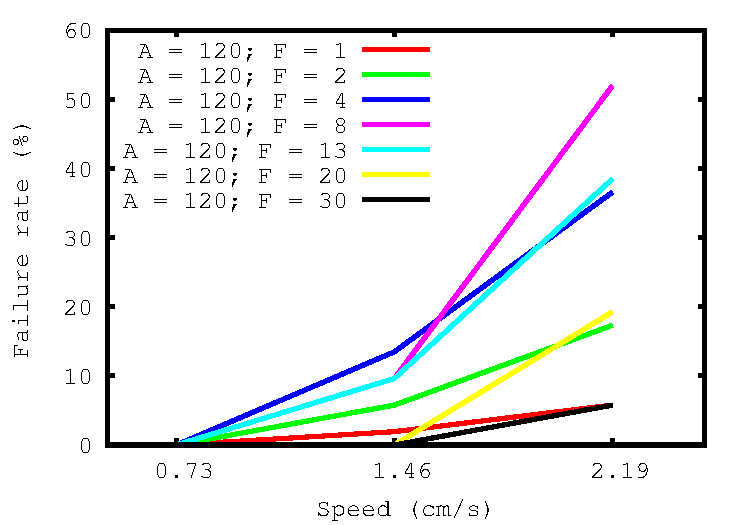
\includegraphics[width=\textwidth]{figures/ch4/speed_angle_120_failures}
			\caption{Taux d'échecs pour $A = 120$.}
			\label{fig:spEffect_f_120}
		\end{subfigure}
		\caption[Effet de la vitesse sur les performances de sélection]{Effet de la vitesse sur les performances de sélection. Les MTSN, taux d'erreurs d'échecs sont présentés pour deux valeurs de A, et pour toutes les valeurs de F que nous avons testées.}
		\label{fig:spEffectPerf}
	\end{figure}


	\subsection{Angle}
	L'effet du paramètre d'angle est plus subtile à interpréter, notamment du fait d'intéractions avec la vitesse et la fréquence. À basse vitesse, l'effet de A sur les MTSN est faible : pour $V = 0,73$ et $F = 4$, quand $A= 0$, $MTSN = 14~\%{}$ alors que quand $A = 120$, $MTSN = 20~\%{}$, soit une différence de pourcentage de seulement 33~\%{}, et qui plus est la plus importante mesurée entre deux valeurs de A pour cette vitesse. En revanche, lorsque S vaut 2,19, alors les MTSN sont respectivement 21~\%{} et 54~\%{} pour les mêmes valeurs de A et F, ce qui représente une différence de pourcentage de 90~\%{}.
	
	L'inteprétation que nous proposons est qu'à basse vitesse, la sélection est de toute façon relativement facile, presque indépendamment de la nature du mouvement, ce qui n'est plus du tout vrai avec des cibles rapides. Ces résultats sont illstrés par la figure~\ref{fig:aEffectPerf}.

	\begin{figure}[!htb]
		\centering
		\begin{subfigure}[t]{\subImgWlineplot}
			\centering
			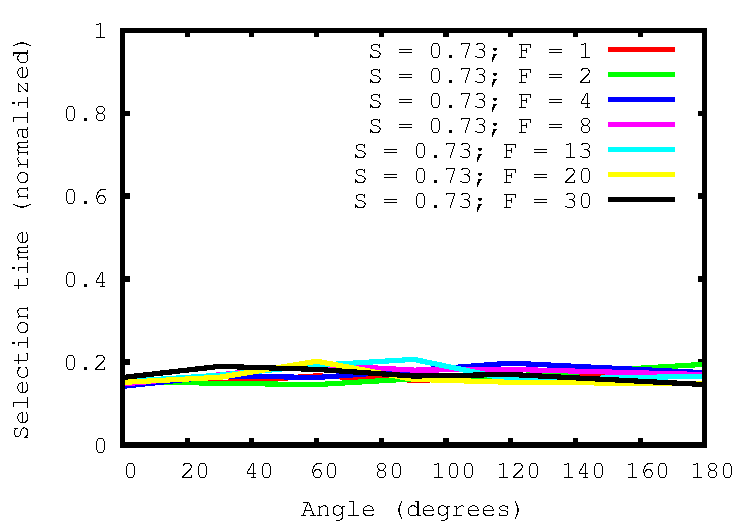
\includegraphics[width=\textwidth]{figures/ch4/angle_speed_0_73_times}
			\caption{MTSN pour $V = 0,73$.}
			\label{fig:aEffect_t_073}
		\end{subfigure}
		~
		\begin{subfigure}[t]{\subImgWlineplot}
			\centering
			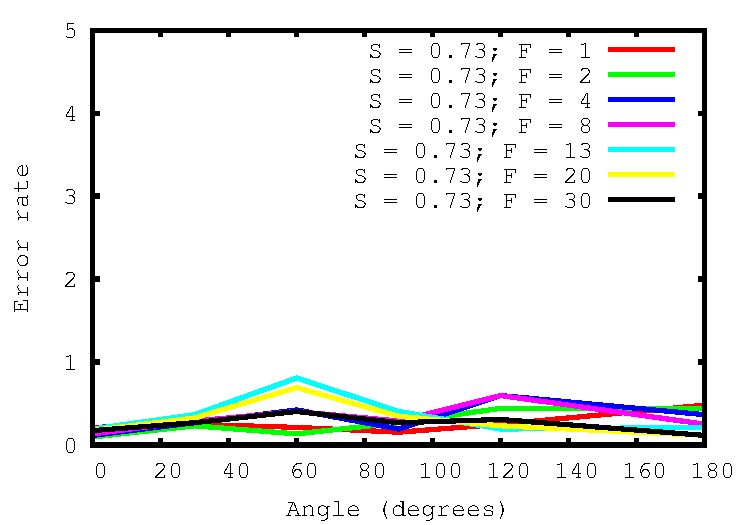
\includegraphics[width=\textwidth]{figures/ch4/angle_speed_0_73_errors}
			\caption{Taux d'erreurs pour $V = 0,73$.}
			\label{fig:aEffect_e_073}
		\end{subfigure}
		~
		\begin{subfigure}[t]{\subImgWlineplot}
			\centering
			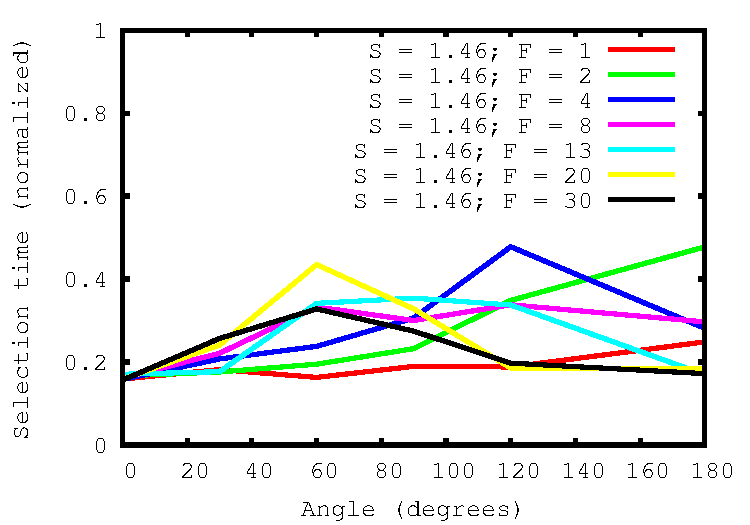
\includegraphics[width=\textwidth]{figures/ch4/angle_speed_1_46_times}
			\caption{MTSN pour $V = 1,46$.}
			\label{fig:aEffect_t_146}
		\end{subfigure}
		~
		\begin{subfigure}[t]{\subImgWlineplot}
			\centering
			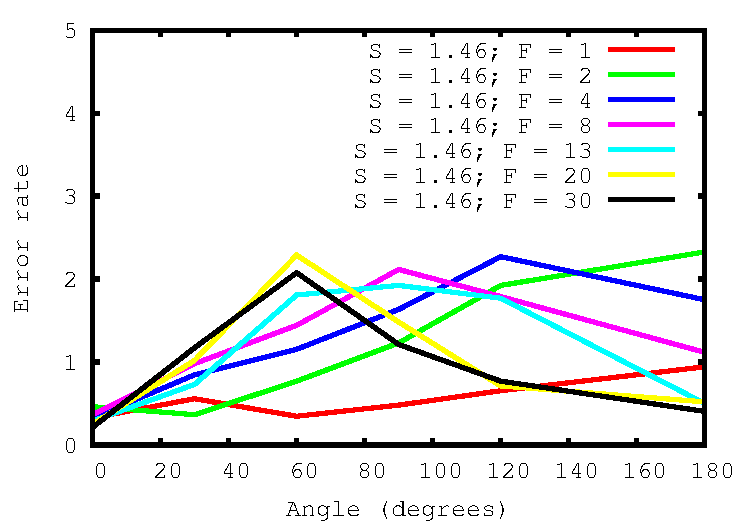
\includegraphics[width=\textwidth]{figures/ch4/angle_speed_1_46_errors}
			\caption{Taux d'erreurs pour $V = 1,46$.}
			\label{fig:aEffect_e_146}
		\end{subfigure}
		~
		\begin{subfigure}[t]{\subImgWlineplot}
			\centering
			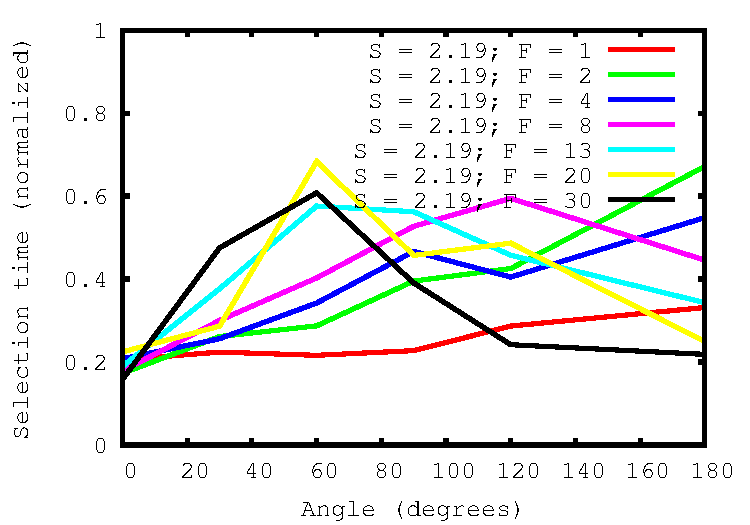
\includegraphics[width=\textwidth]{figures/ch4/angle_speed_2_19_times}
			\caption{MTSN pour $V = 2,19$.}
			\label{fig:aEffect_t_219}
		\end{subfigure}
		~
		\begin{subfigure}[t]{\subImgWlineplot}
			\centering
			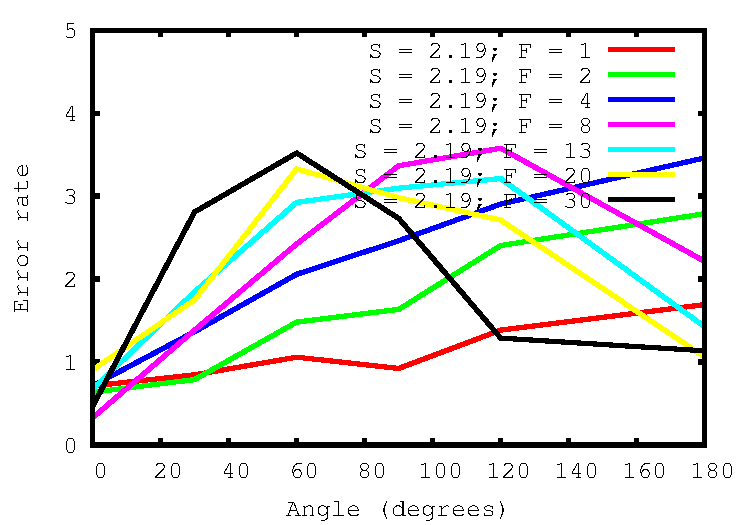
\includegraphics[width=\textwidth]{figures/ch4/angle_speed_2_19_errors}
			\caption{Taux d'erreurs pour $V = 2,19$.}
			\label{fig:aEffect_e_219}
		\end{subfigure}
		\caption[Effet du paramètre d'angle sur les performances de sélection]{Effet du paramètre d'angle sur les performances de sélection. Les MTSN et taux d'erreurs sont présentés pour toutes les valeurs de V et de F que nous avons testées. Comme on le voit, les interactions sont fortes entre les différents paramètres, et les effets de A et F sont d'autant plus marqués que V est grande.}
		\label{fig:aEffectPerf}
	\end{figure}
	
	En particulier, la figure~\ref{fig:aEffect_t_219} montre l'effet de A sur les MTSN à haute vitesse. Observons que tant que la fréquence est basse, de faibles valeurs de A sont associées à de faibles MTSN ; mais lorsque F croît, l'effet de A sur les temps de sélection change : les MTSN croissent d'abord avec A, atteignent un plateau, puis décroissent.
	
	De plus, la valeur de A associée à ce plateau ($A_{pic}$) dépend de A : plus F est grande, plus $A_{pic}$ est petit. Les erreurs et les échecs (omis ici) suivent la même tendance, mais les effets sont dépendants de la vitesse (d'autant plus forts qu'elle est élevée).

	\subsection{Fréquence}
	Les tendances sont similaires pour la fréquence : F a un plus petit impact sur le temps de sélection lorsque la vitesse est basse, et plus grand quand elle est élevée. Sur la figure~\ref{fig:fEffectPerf}, on observe que lorsque A est faible, les fortes valeurs de F sont corrélées avec de longs temps de sélection. Mais pour de fortes valeurs de A, la tendance change : quand A est grand, la MTSN croît avec F jusqu'à une certaine valeur ($F_{pic}$), puis décroît. De plus, la valeur de $F_{pic}$ diminue quand A augmente. Les TERR et TECH suivent la même tendance que les MTSN.
	
	L'effet de F est donc approximativement symétrique de celui de A, et comme pour A, il est d'autant plus prononcé que la vitesse est élevée.

	\begin{figure}[!htb]
		\centering
		\begin{subfigure}[t]{\subImgWlineplot}
			\centering
			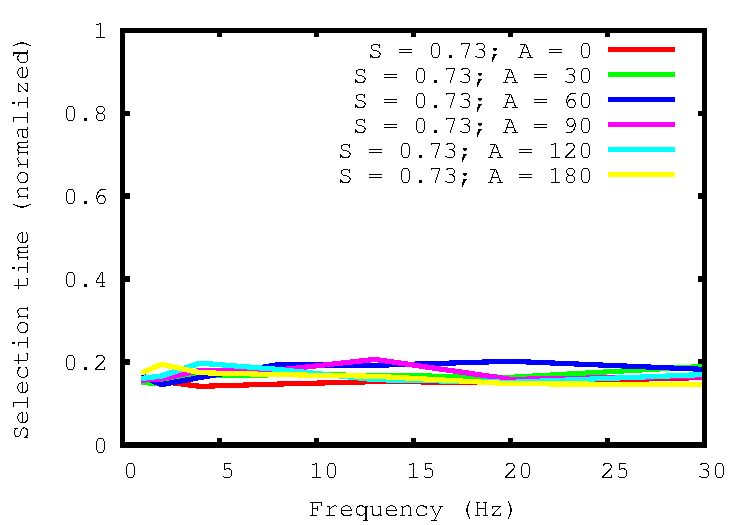
\includegraphics[width=\textwidth]{figures/ch4/frequency_speed_0_73_times}
			\caption{MTSN pour $V = 0,73$.}
			\label{fig:fEffect_t_073}
		\end{subfigure}
		~
		\begin{subfigure}[t]{\subImgWlineplot}
			\centering
			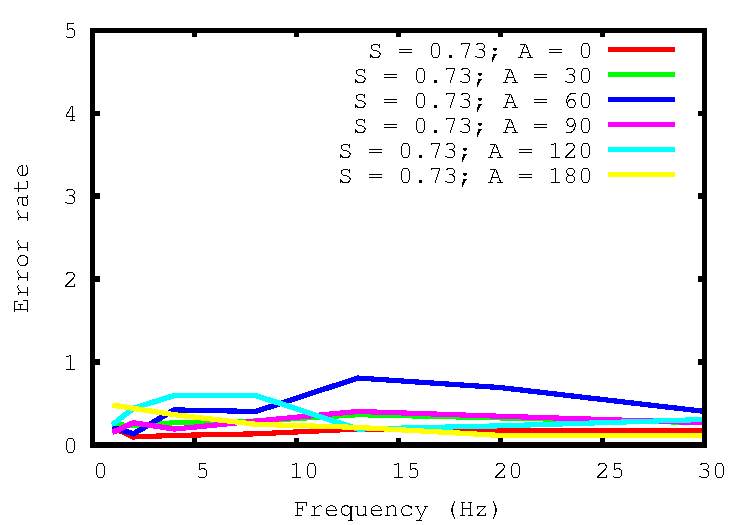
\includegraphics[width=\textwidth]{figures/ch4/frequency_speed_0_73_errors}
			\caption{Taux d'erreurs pour $V = 0,73$.}
			\label{fig:fEffect_e_073}
		\end{subfigure}
		~
		\begin{subfigure}[t]{\subImgWlineplot}
			\centering
			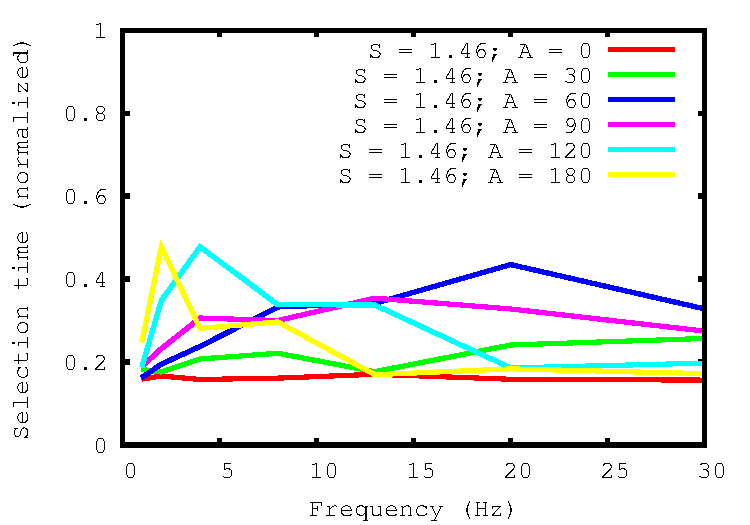
\includegraphics[width=\textwidth]{figures/ch4/frequency_speed_1_46_times}
			\caption{MTSN pour $V = 1,46$.}
			\label{fig:fEffect_t_146}
		\end{subfigure}
		~
		\begin{subfigure}[t]{\subImgWlineplot}
			\centering
			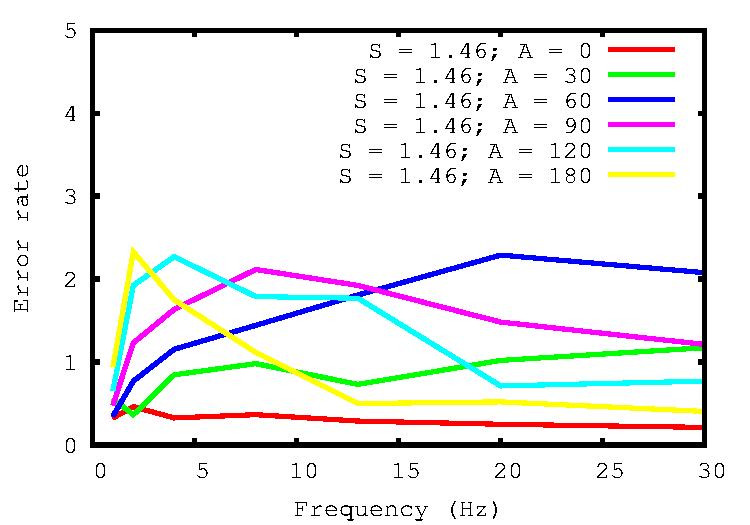
\includegraphics[width=\textwidth]{figures/ch4/frequency_speed_1_46_errors}
			\caption{Taux d'erreurs pour $V = 1,46$.}
			\label{fig:fEffect_e_146}
		\end{subfigure}
		~
		\begin{subfigure}[t]{\subImgWlineplot}
			\centering
			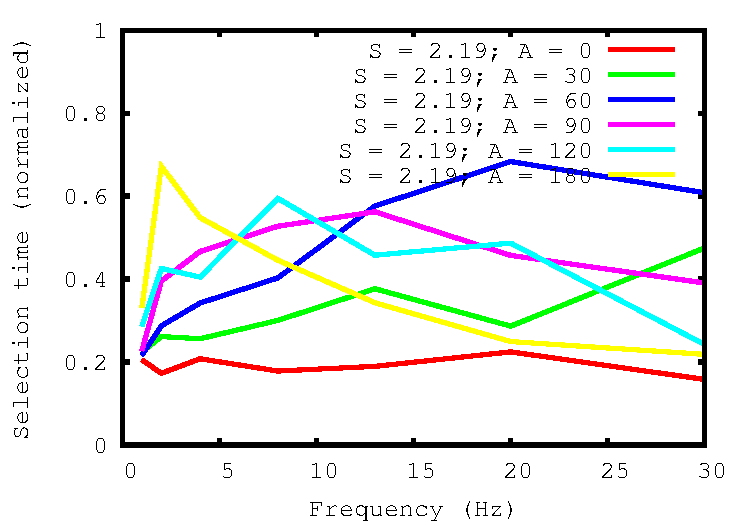
\includegraphics[width=\textwidth]{figures/ch4/frequency_speed_2_19_times}
			\caption{MTSN pour $V = 2,19$.}
			\label{fig:fEffect_t_219}
		\end{subfigure}
		~
		\begin{subfigure}[t]{\subImgWlineplot}
			\centering
			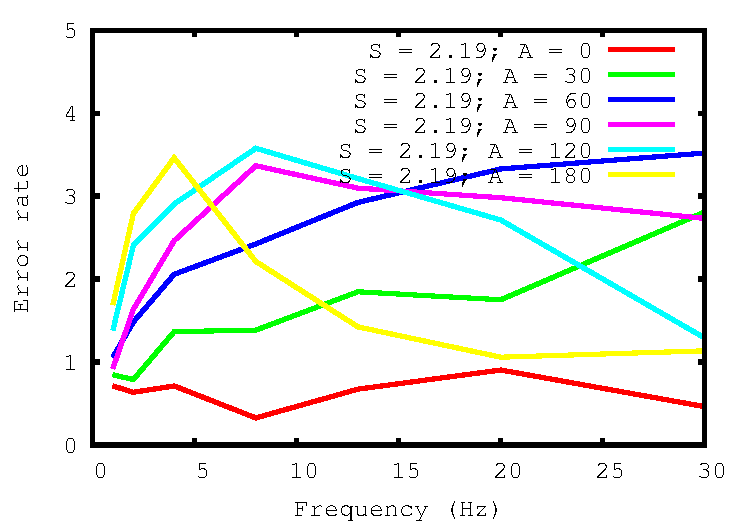
\includegraphics[width=\textwidth]{figures/ch4/frequency_speed_2_19_errors}
			\caption{Taux d'erreurs pour $V = 2,19$.}
			\label{fig:fEffect_e_219}
		\end{subfigure}
		\caption[Effet de la fréquence sur les performances de sélection]{Effet de la fréquence sur les performances de sélection. Les MTSN et taux d'erreurs sont présentés pour toutes les valeurs de V et de A que nous avons testées. Comme on le voit, les interactions sont fortes entre les différents paramètres, et les effets de A et F sont d'autant plus marqués que V est grande.}
		\label{fig:fEffectPerf}
	\end{figure}

\section{Analyse exploratoire}
	Nous avons également porté un regard sur notre espace de paramètres entier afin d'identifier des tendances plus générales.

	Les cartes thermiques (\emph{heat maps}) sur les figures~\ref{fig:hmap_t_146} et~\ref{fig:hmap_t_219} présentent les MTSN pour toutes les combinaisons de A et F aux vitesses intermédiaire et élevée, respectivement. Sur chaque carte, A se lit sur l'axe des abscisses, et F sur celui des ordonnées. Les TERR et TECH sont également représentés sur la figure~\ref{fig:hmaps}.
	
	Nous remarquons sur toutes ces cartes de chaleur --- et plus clairement à 2,19~cm/s --- qu'une zone approximativement située sur la diagonale principale (du coin supérieur gauche au coin inférieur droit) est associé aux MTSN, TERR et TECH les plus élevés, donc aux conditions les plus difficiles.
	
	Si l'on suit cette diagonale et que l'on se rapporte aux axes des abscisses et des ordonnées, l'on peut remarquer qu'elle est caractérisée soit par une forte valeur de A associée à une faible valeur de F, soit l'inverse, soit à des valeurs de A et F simultanément intermédiaires.
	
	Inversement, lorsque A et F sont simultanément faibles (coin inférieur gauche) ou simultanément élevés (coin supérieur droit) la sélection est relativement aisée.

	\begin{figure}[!htb]
		\centering
		\begin{subfigure}[t]{\subImgWlineplot}
			\centering
			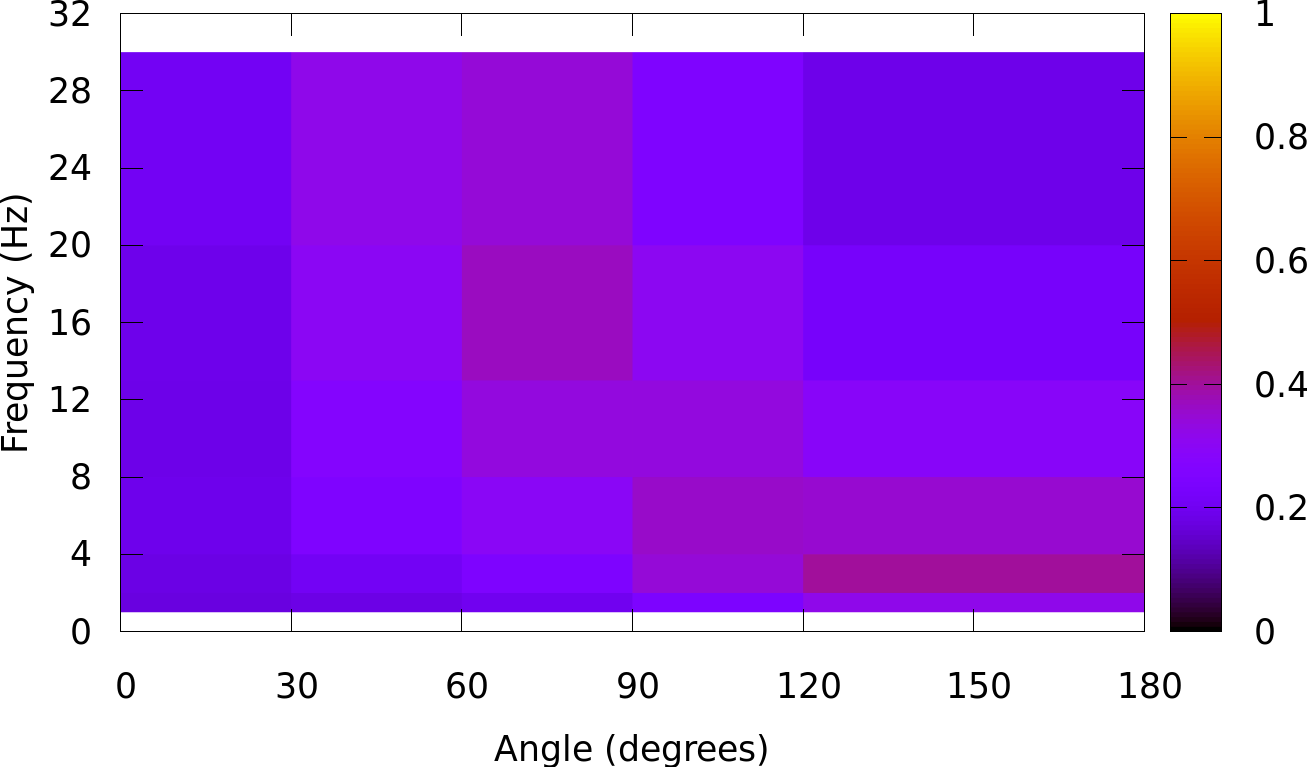
\includegraphics[width=\textwidth]{figures/ch4/average_times_054}
			\caption{MTSN pour $V = 1,46$.}
			\label{fig:hmap_t_146}
		\end{subfigure}
		~
		\begin{subfigure}[t]{\subImgWlineplot}
			\centering
			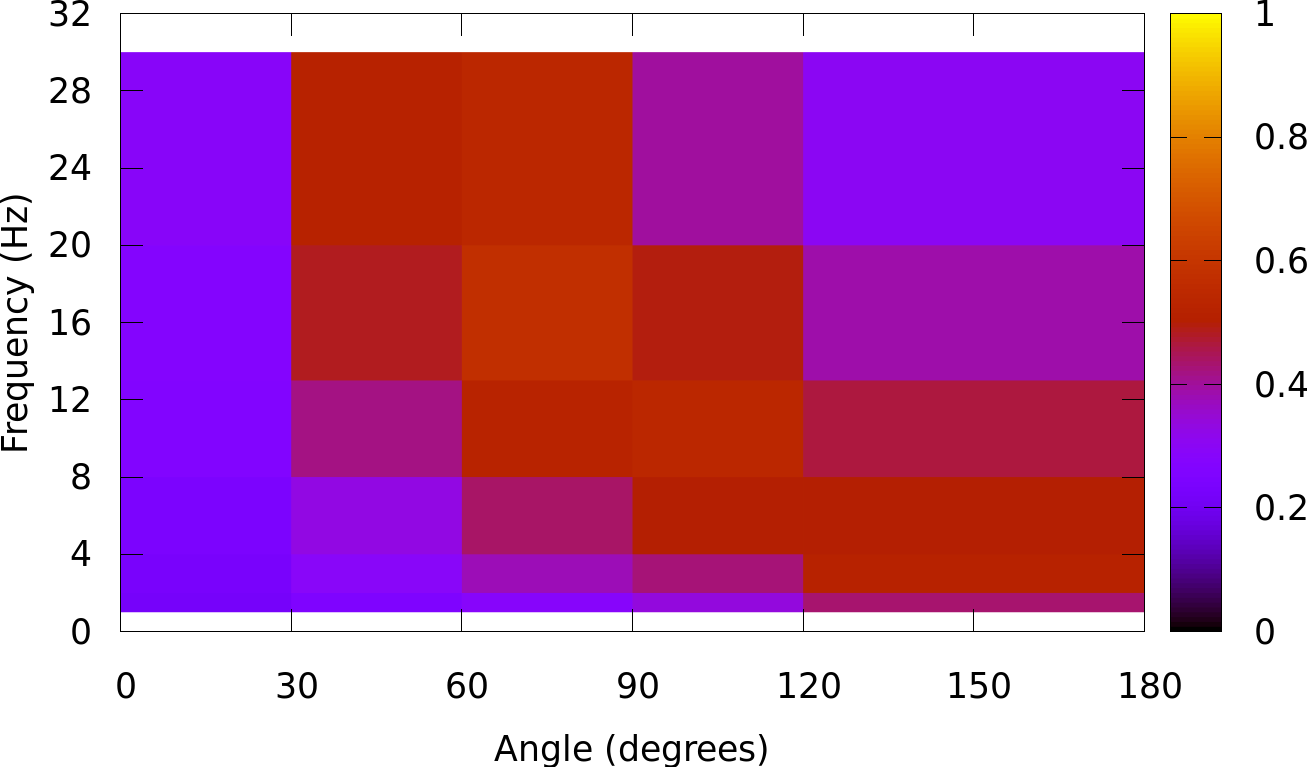
\includegraphics[width=\textwidth]{figures/ch4/average_times_081}
			\caption{MTSN pour $V = 2,19$.}
			\label{fig:hmap_t_219}
		\end{subfigure}
		~
		\begin{subfigure}[t]{\subImgWlineplot}
			\centering
			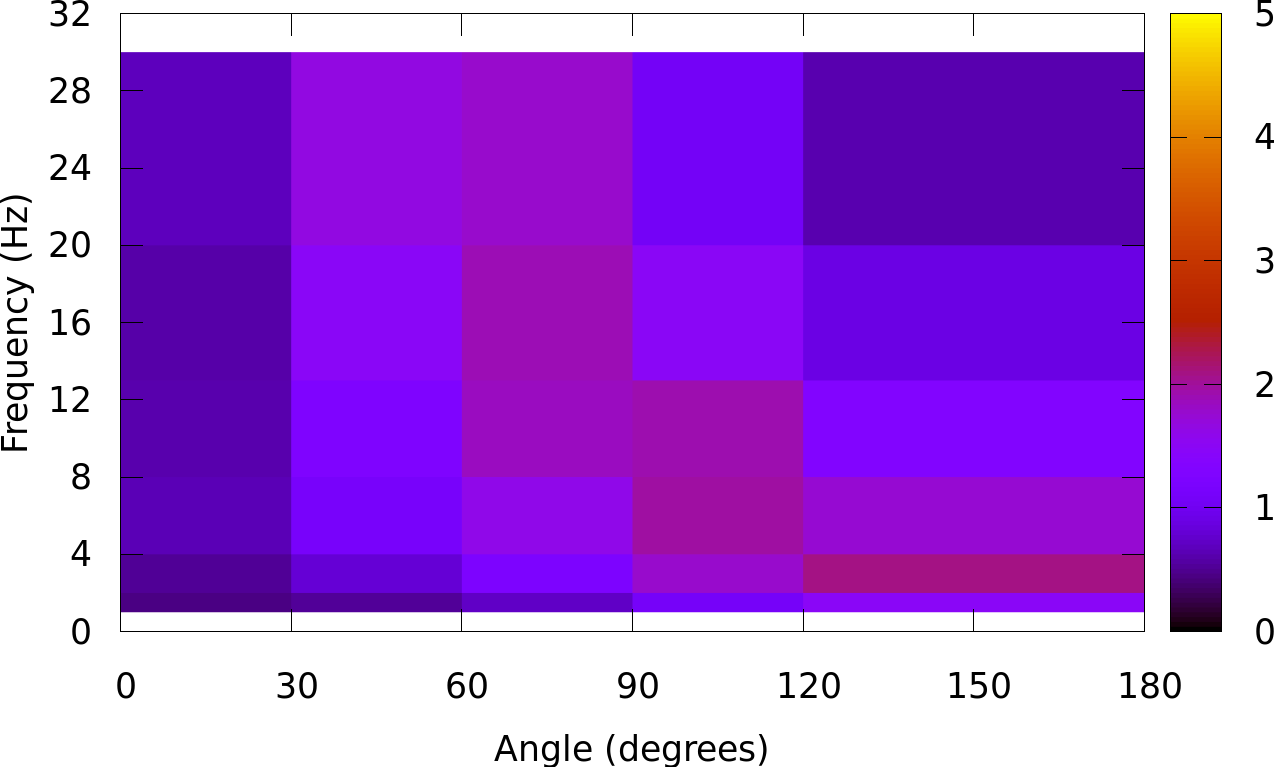
\includegraphics[width=\textwidth]{figures/ch4/average_error_rates_054}
			\caption{Taux d'erreurs pour $V = 1,46$.}
			\label{fig:hmap_e_146}
		\end{subfigure}
		~
		\begin{subfigure}[t]{\subImgWlineplot}
			\centering
			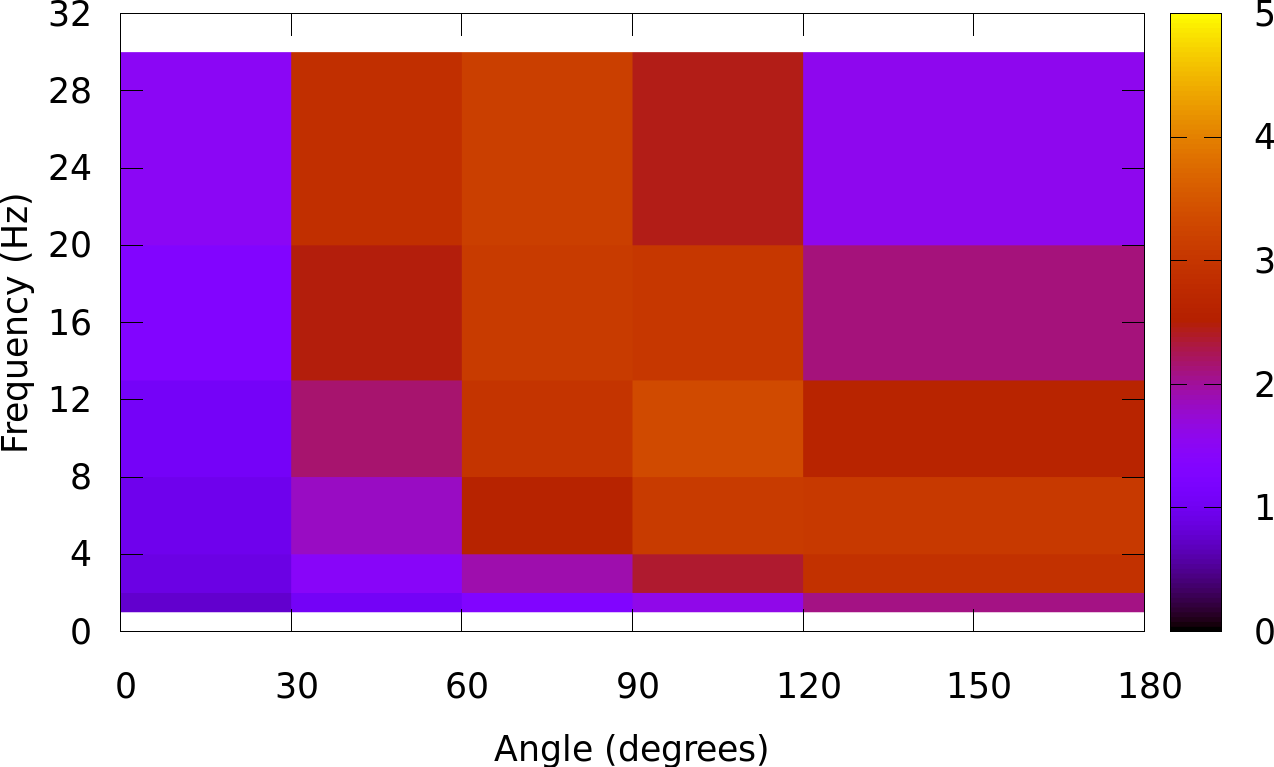
\includegraphics[width=\textwidth]{figures/ch4/average_error_rates_081}
			\caption{Taux d'erreurs pour $V = 2,19$.}
			\label{fig:hmap_e_219}
		\end{subfigure}
		~
		\begin{subfigure}[t]{\subImgWlineplot}
			\centering
			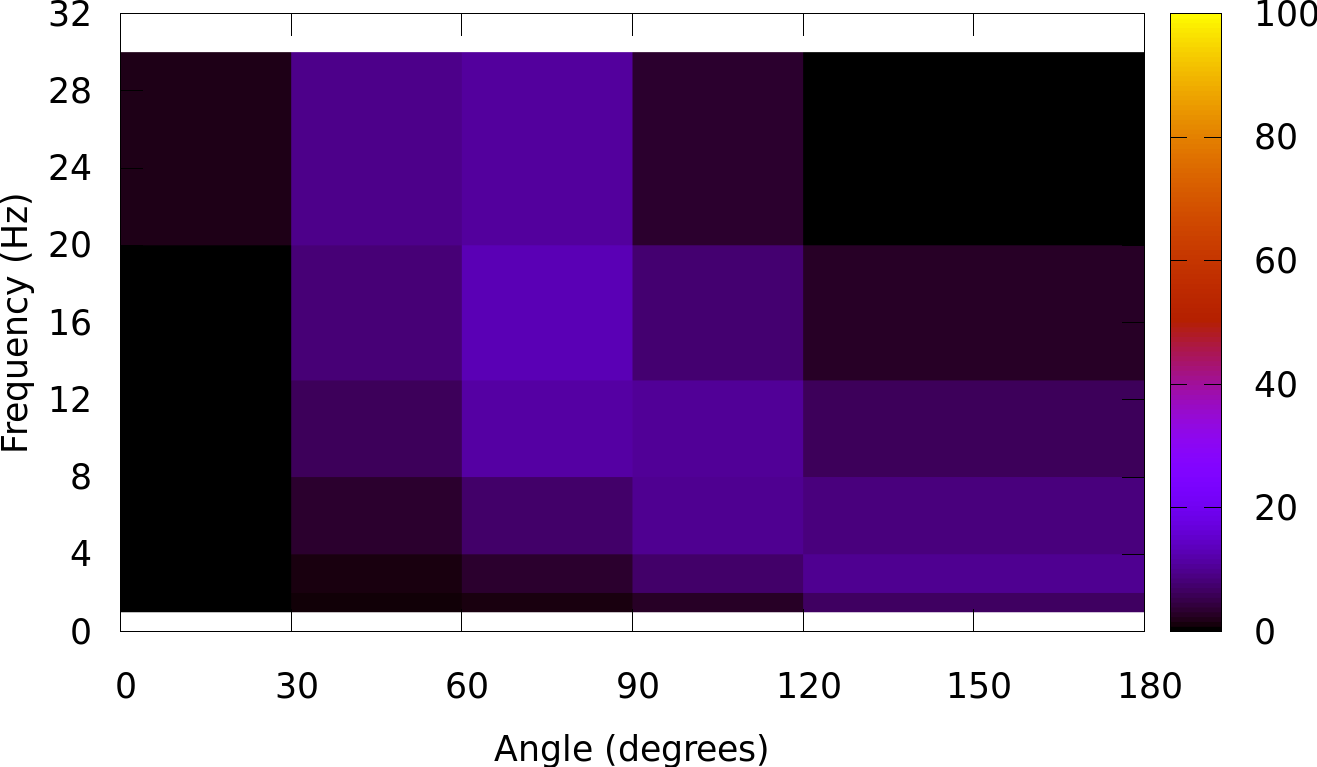
\includegraphics[width=\textwidth]{figures/ch4/average_failure_rates_054}
			\caption{Taux d'échecs pour $V = 2,19$.}
			\label{fig:hmap_f_146}
		\end{subfigure}
		~
		\begin{subfigure}[t]{\subImgWlineplot}
			\centering
			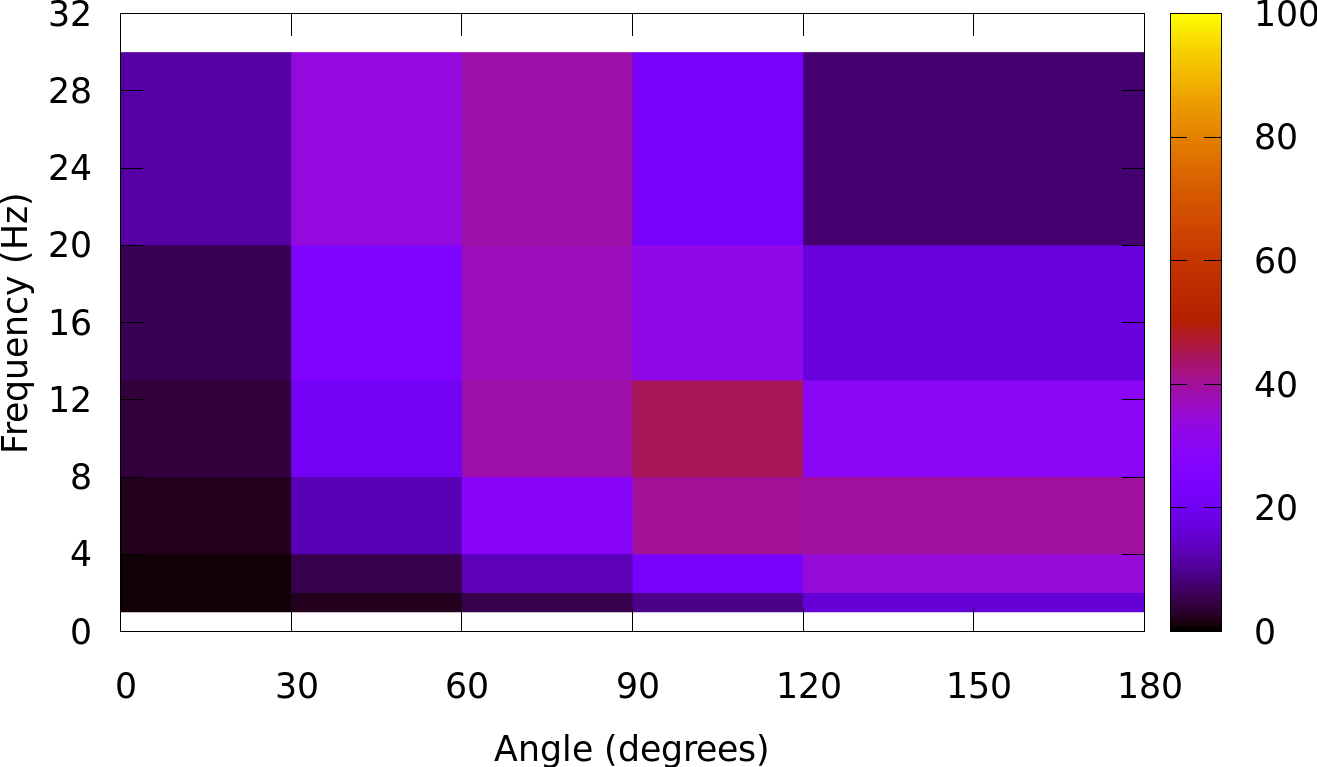
\includegraphics[width=\textwidth]{figures/ch4/average_failure_rates_081}
			\caption{Taux d'échecs pour $V = 2,19$.}
			\label{fig:hmap_f_219}
		\end{subfigure}
		\caption[Effets combinés de F et A sur les performances de sélection]{Effets combinés de F et A sur les performances de sélection. Les MTSN, TERR et TECH sont présentés pour toutes les valeurs de F et de A que nous avons testées, à moyenne et haute vitesse. Ces cartes thermiques (\emph{heat maps}) utilisent la couleur pour représenter une grandeur, selon l'échelle indiquée à leur droite. Les valeurs de A se lisent en abscisse, et celles de F en ordonnée. Ainsi, pour une vitesse données, toutes les combinaisons de A et F sont représentées.}
		\label{fig:hmaps}
	\end{figure}

	\subsection{Prévisibilité selon les angles et fréquences}
	Les tendances observées ci-dessus suggèrent que le produit de A et F (appelé pseudo-entropie dans le chapitre~\ref{chap3}) pourrait prédire les performances de sélection de cibles mobiles avec quelque efficacité. Nous avons tracé un graphique de la MTSN en fonction du produit AF, mettant en lumière les tendances observées pour A et F séparément, et leurs interactions, voir la figure~\ref{fig:tAF}.
	
	Plus spécifiquement, lorsque AF atteint une certaine valeur $AF_{pic}$ (ici située autour de 1100), le temps de sélection est maximal. Nous supposons que $AF_{pic}$ pourrait dépendre de plusieurs paramètres, tels que la largeur ou l'amplitude de Fitts, mais cette valeur est stable aux trois vitesses que nous avons évaluées, aussi en est-elle probablement indépendante. Naturellement, les tendances observées pour les MTSN valent également pour les TERR et TECH, très fortement corrélés aux MTSN (le coefficient de corrélation de Pearson entre les MTSN et TERR est supérieur à 0,959, avec une \emph{p-value} inférieure à $10^{-69}$).
	
	La figure~\ref{fig:tAF_Spnorm} présente $\frac{MTSN}{V}$, c'est-à-dire la MTSN normalisée par rapport à la vitesse, en fonction de AF. Les effets de AF étant trop faibles à basse vitesse, ils sont omis sur cette figure, et seules les vitesses moyenne et haute sont préservées.
	
	\begin{figure}[!htb]
		\begin{subfigure}[t]{0.49\textwidth}
			\centering
			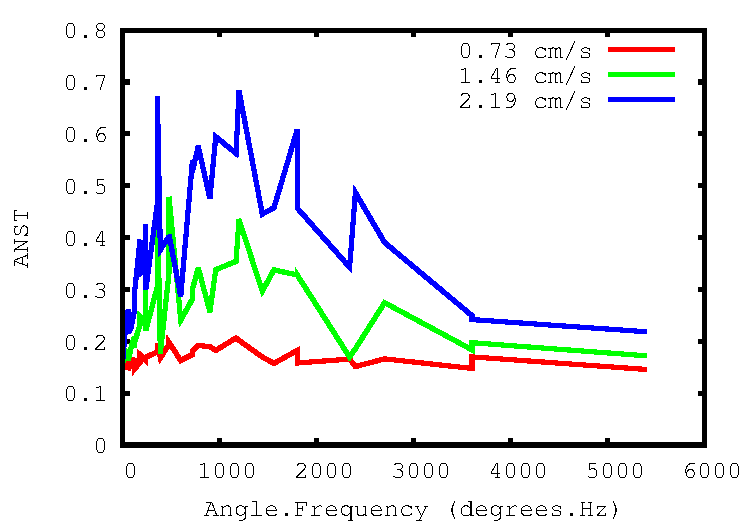
\includegraphics[width=\textwidth]{figures/ch4/time_vs_AF_all_speeds}
			\caption{MTSN en fonction du produit AF, pour chaque vitesse.}
			\label{fig:tAFallSp}
		\end{subfigure}
		~
		\begin{subfigure}[t]{0.49\textwidth}
			\centering
			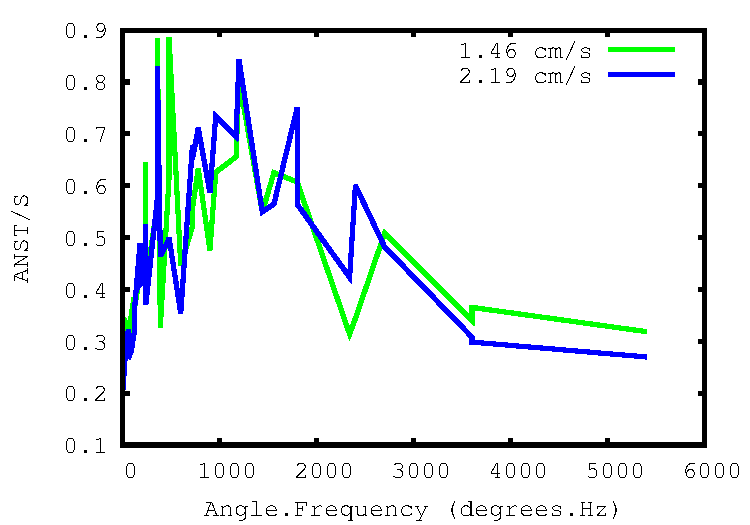
\includegraphics[width=\textwidth]{figures/ch4/time_vs_AF_all_speeds_normalized}
			\caption{$MTSN/V$ en fonction du produit AF, à moyenne et haute vitesse.}
			\label{fig:tAF_Spnorm}
		\end{subfigure}
		~
		\begin{subfigure}[t]{\textwidth}
			\centering
			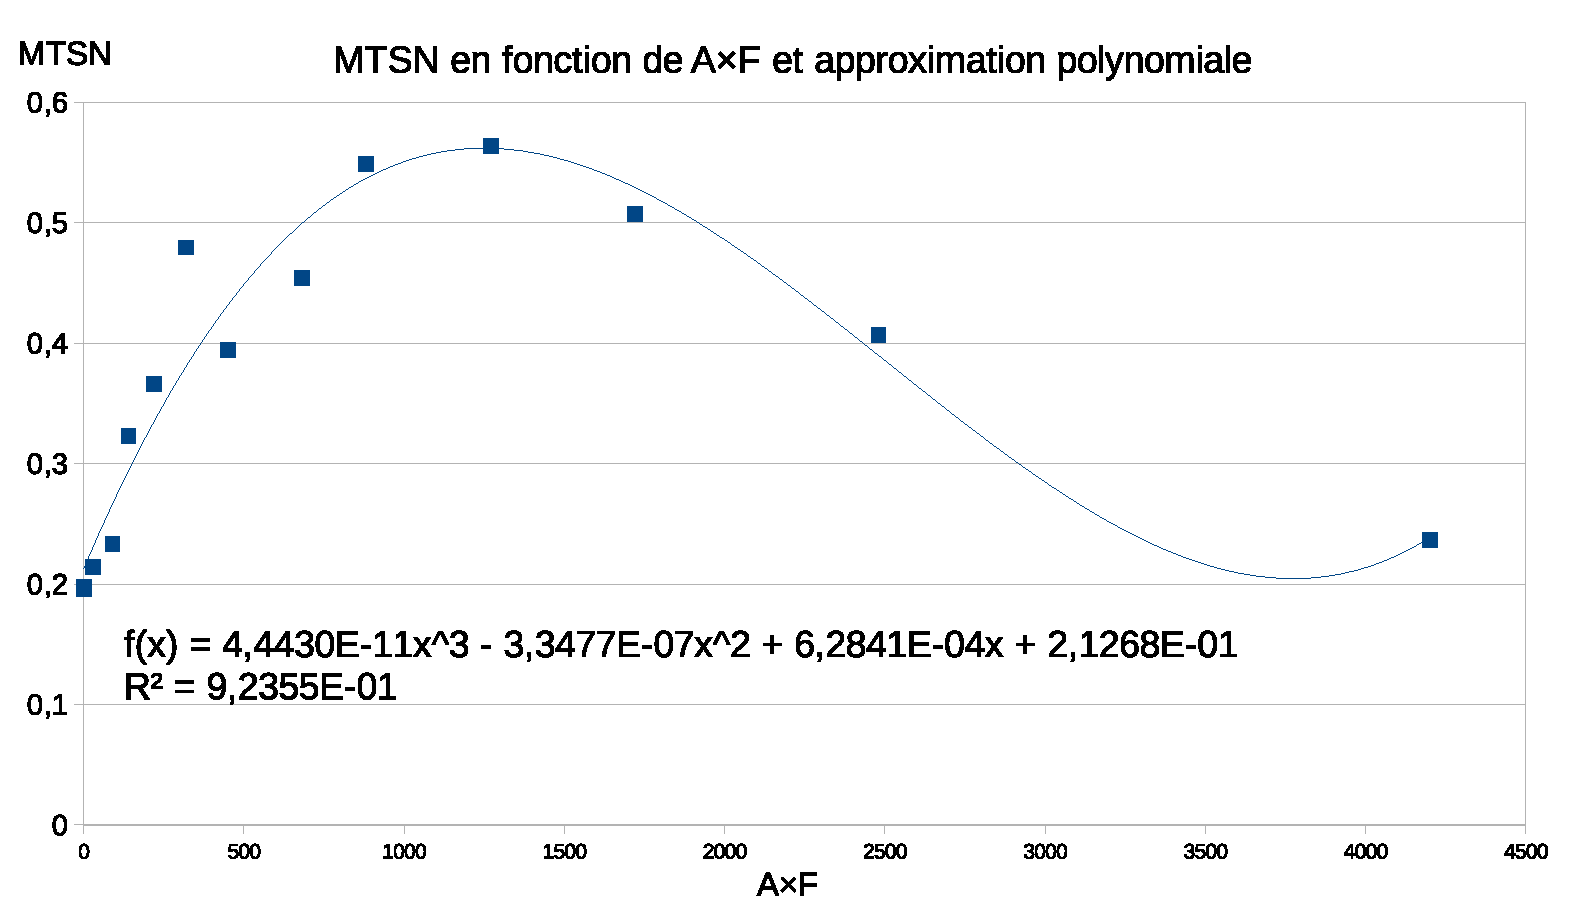
\includegraphics[width=\textwidth]{figures/ch4/MTSNvAF}
			\caption{MTSN sur les cibles rapides en fonction du produit AF après lissage, et approximation polynomiale (cubique). Le coefficient de détermination est légèrement supérieur à 92~\%{}, mais la croissance du polynome à partir de $AF \approx 3750$ montre bien que ce modèle ne peut être utile que sur un intervalle borné.}
			\label{fig:tAF_smooth}
		\end{subfigure}
		\caption[MTSN en fonction du produit AF]{MTSN en fonction du produit AF.}
		\label{fig:tAF}
	\end{figure}
	
	Comme on le constate, les courbes se superposent --- ce qui est assez logique compte tenu de l'effet approximativement linéaire de la vitesse sur les MTSN observé plus haut. Pour une vitesse donnée, la pseudo-entropie paraît donc offrir un moyen d'estimer la difficulté de sélection, par exemple en calculant la distance entre le produit AF d'une condition et la valeur $AF_{pic}$, si elle est connue.
	
	Nous proposons également un modèle très simple permettant d'estimer le temps de sélection en fonction du produit AF, sous la forme d'un polynome cubique, illustré sur la figure~\ref{fig:tAF_smooth}. Il est cependant évident, du fait de la croissance de ce polynome après $AF \approx 3750$, que le champ d'application de ce modèle doit être limité à $AF \in [0, 3000]$, approximativement. L'on pourrait d'ailleurs se contenter d'un polynome quadratique sur cet intervalle, au prix d'une légère perte de précision ($R^{2} \approx 88,6~\%{}$).
	
	\subsubsection{Variations individuelles}
	La discussion de ces résultats ne serait pas complète sans préciser que même si la \og diagonale de difficulté \fg{} est observable et stable dans les résultats de tous nos sujets, les conditions les plus difficiles ne sont pas toujours les mêmes, quoiqu'elles soient toujours sur ladite diagonale. La figure~\ref{fig:tVariation} illustre ces variations, en s'appuyant sur l'exemple de deux sujets.
	
	\begin{figure}[!htb]
		\begin{subfigure}[t]{0.49\textwidth}
			\centering
			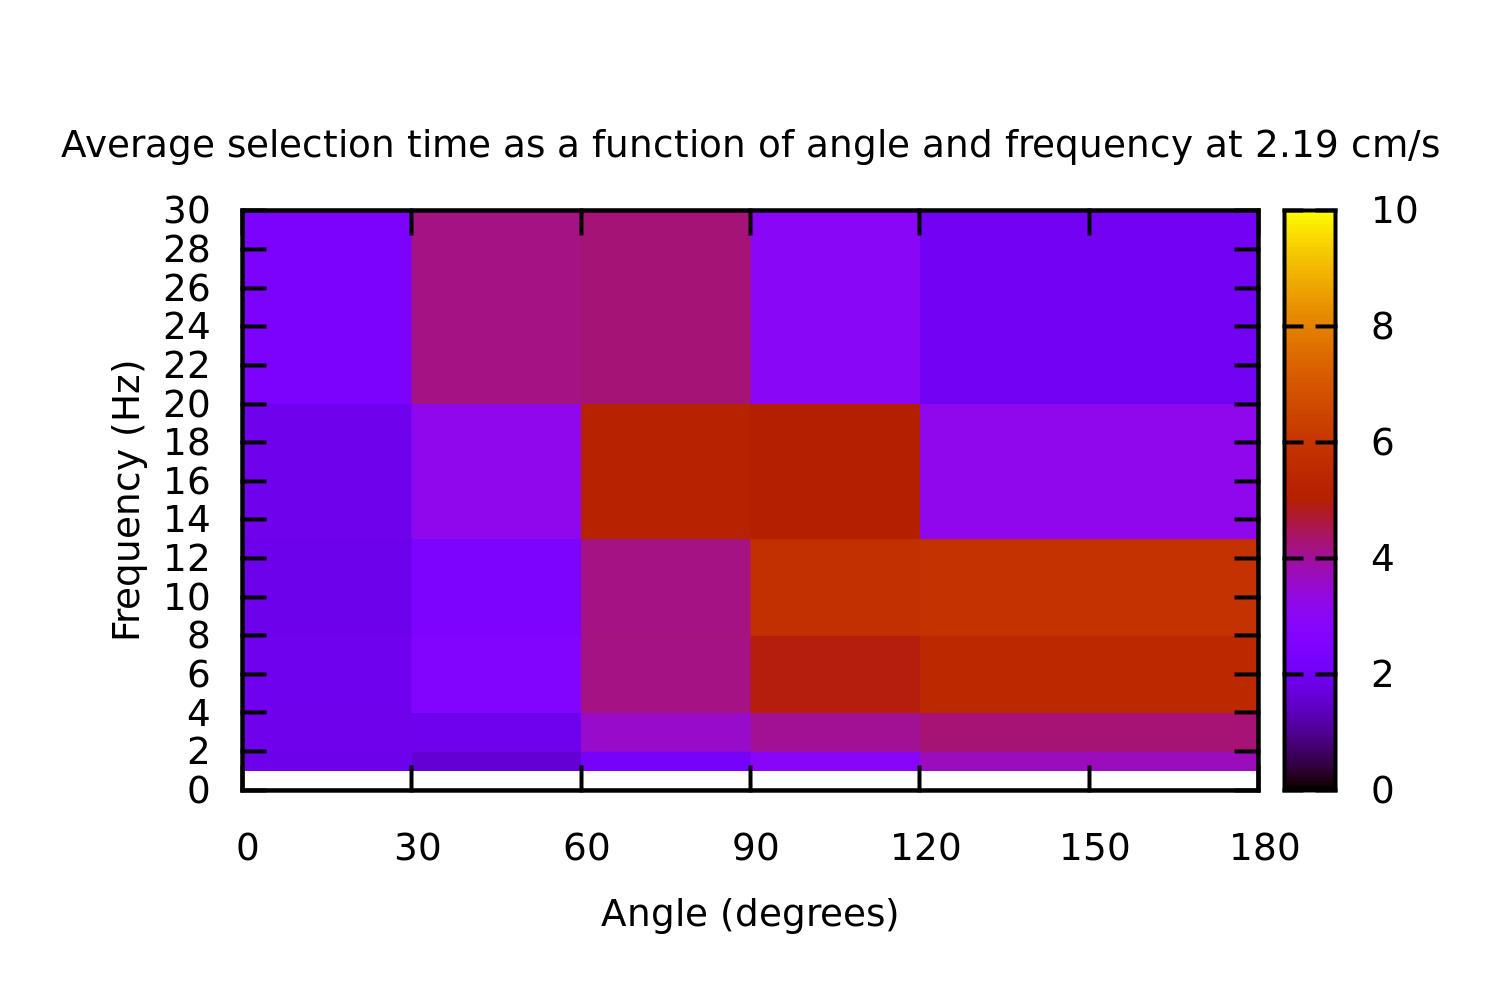
\includegraphics[width=\textwidth]{figures/ch4/08_times_081}
			\caption{Temps de sélection en fonction de A et F pour un sujet.}
			\label{fig:08times}
		\end{subfigure}
		~
		\begin{subfigure}[t]{0.49\textwidth}
			\centering
			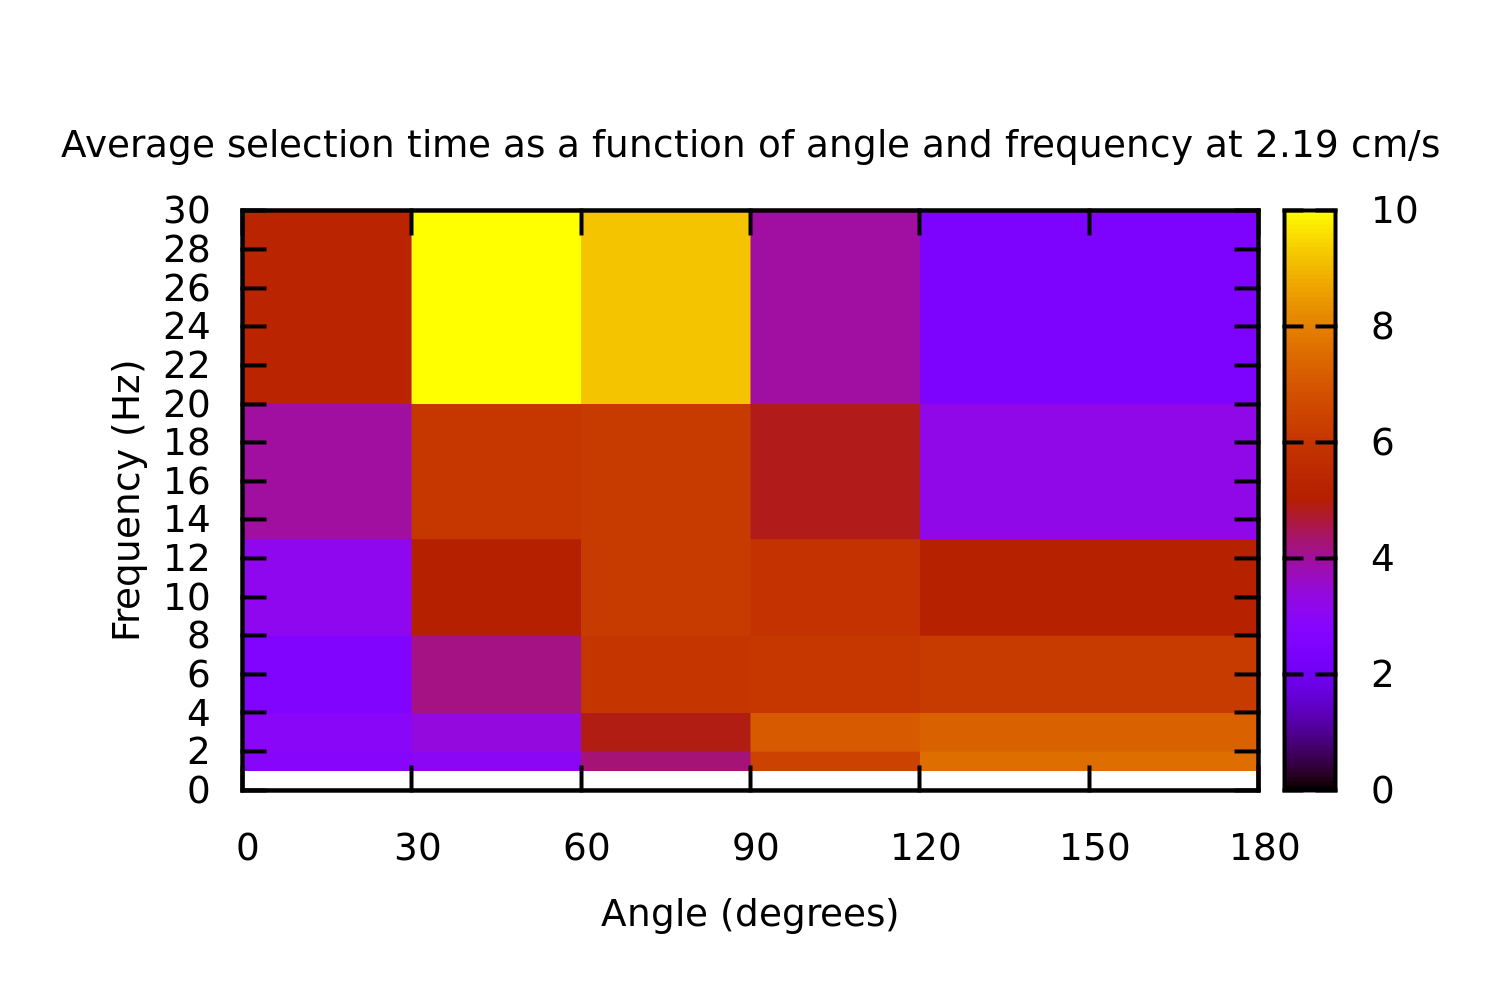
\includegraphics[width=\textwidth]{figures/ch4/09_times_081}
			\caption{Temps de sélection en fonction de A et F pour un autre sujet.}
			\label{fig:09times}
		\end{subfigure}
		\caption[Variations entre les sujets]{Temps de sélection (en secondes) en fonction de A et F pour deux sujets différents, à vitesse élevée. Dans les deux cas, la \og diagonale de difficulté \fg{} est identifiable mais la condition la plus difficile pour le sujet de droite est relativement aisée pour celui de gauche, qui a eu plus de mal avec la partie basse de la diagonale.}
		\label{fig:tVariation}
	\end{figure}
	
	Dans les deux cas, des valeurs de AF intermédiaires (qui caractérisent la diagonale de difficulté) sont associés aux conditions les plus difficiles ; mais pour un sujet, ce sont les basses fréquences accompagnées de grands angles qui posent le plus de problèmes (figure~\ref{fig:08times}), tandis que pour l'autre, ce sont les hautes fréquences accompagnées de petits angles (figure~\ref{fig:09times}). Il est difficile de dire d'où proviennent ces différences.
	
	Observons cependant que le sujet de la figure~\ref{fig:08times} a obtenu, globalement, de bien meilleures performances que celui de la figure~\ref{fig:09times}. Cependant nos sujets les plus lents n'ont pas nécessairement rencontré leurs difficultés maximales sur cette zone de la diagonale de difficulté, et ne sont pas assez nombreux pour que nous puissions en tirer des résultats significatifs.

	\subsection{Impressions subjectives}
	Les réponses au questionnaire que nous avons soumis à nos sujets sont cohérentes avec nos mesures quantitatives, et apportent des précisions complémentaires. En effet, 92~\%{} des sujets furent capables d'identifier plusieurs catégories de mouvement, et 77~\%{} d'entre eux purent en identifier au moins trois, accompagnées de deux ou trois stratégies de sélection correspondantes.
	
	\subsubsection{Catégories et stratégies}
	\paragraph{Catégories.}
	Nos sujets ont d'abord décrit une première forme de mouvement \og stable \fg{} (et parfois qualifié de \og prévisible \fg{}), caractérisé par des lignes approximativement droites, avec des changements de directions faibles ou rares. Il est intéressant d'observer qu'un sujet précisa que les changements de direction survenaient \og toutes les deux secondes \fg{}, ce qui impliquerait $F = 0,5$~Hz quand la valeur minimale de F testée était 1~Hz. Peut-être la concentration intense perturbe-t-elle la perception du temps\ldots{} Les descriptions détaillées fournies par nos sujets nous permettent de relier cette catégorie aux condition pour lesquelles AF est faible (les coins inférieurs gauches de nos cartes thermiques, figure~\ref{fig:hmaps}). Appelons cette catégorie \emph{stable}.
	
	Une seconde forme de mouvement fut identifiée, qualifiée de \og saccadée \fg{}, \og irrégulière \fg{} ou encore \og imprévisible \fg{}. Plus précisément, nos sujets mentionnèrent des changements de direction fréquents et importants. Ces indications nous permettent d'associer cette catégorie aux conditions de valeur AF intermédiaire, situées sur la \og diagonale de difficulté \fg{} de nos cartes thermiques. Appelons cette catégorie \emph{saccadée}.
	
	Enfin, une troisième catégorie fut identifiée, qualifiée de \og brownienne \fg{} par certains sujets, ou de \og vibratoire \fg{} ; certains évoquèrent des \og oscillations \fg{}. Ces descriptions indiquent clairement qu'il s'agit d'un mouvement caractérisé par un produit AF important, c'est-à-dire des conditions des coins supérieurs droits sur nos cartes thermiques. Appelons cette catégorie \emph{vibratoire}.
	
	Pour une impression plus visuelle de ces catégories, le lecteur peut se référer aux figures~\ref{fig:motion1530}, \ref{fig:motion4560}, \ref{fig:motion7590}, \ref{fig:motion105120}, \ref{fig:motion135150} et \ref{fig:motion165180} et aux valeurs de A et F indiquées dans leurs légendes.
	
	\paragraph{Stratégies de sélection.}
	Il est particulièrement intéressant de noter que 92~\%{} de nos sujets rapportèrent qu'ils essayaient d'anticiper les mouvements de leur cible et de l'intercepter, et ceux d'entre eux qui avaient identifié une catégorie stable ont tous précisé que cette stratégie lui était spécifiquement associée.
	
	Cependant, aucun de nos sujets ne put trouver de stratégie particulièrement efficace pour la catégorie saccadée, et nous ont simplement expliqué qu'ils avaient tenté d'être assez rapides et de cliquer beaucoup --- faisant de fait de nombreuses erreurs. Ceci corrobore nos mesures quantitatives, qui montrent que cette catégorie présente des difficultés considérables.
	
	Pour la catégorie vibratoire, 69~\%{} de nos sujets expliquèrent qu'ils avaient cherché à identifier la position \og moyenne \fg{} de la cible sur une courte période, soit pour intercepter la cible au prochain passage espéré par cette position, soit pour cliquer beaucoup sur et autour de cette zone, dans l'espoir qu'une tentative fût fructueuse.

	\subsubsection{Interprétation}
	Comme précisé plus haut, la catégorie stable correspond aux faibles valeurs de AF, la catégorie saccadée aux valeurs intermédiaires, et la catégorie vibratoires aux fortes valeurs. Il s'agit respectivement des coins inférieurs gauches, de la diagonale principale, et des coins supérieurs droits de nos cartes thermiques.
	
	Ce qu'il est important de remarquer est qu'une stratégie d'anticipation/interception nécessite un certain degré de prévisibilité, car l'on ne peut anticiper de manière fiable que ce que l'on peut prédire. Or, le simple fait de viser la \og position moyenne \fg{} d'une cible sur une courte période est une prédiction en soi, c'est faire l'hypothèse que la cible repassera vite par cet endroit.
	
	En revanche, la catégorie saccadée semble très difficile à prédire, à tel point qu'aucun de nos sujets n'a rapporté avoir cherché à anticiper ou prédire de tels mouvements pour sélectionner une cible de cette catégorie. Nous en déduisons que les catégories stable et vibratoire sont caractérisées par des sélections relativement aisées du fait de la nature prévisible de leurs mouvements, tandis que la catégorie saccadée est caractérisée par des sélections difficiles du fait de la nature imprévisible de ses mouvements.
	
	Cette observation peut paraître quelque peu contre-intuitive pour la catégorie vibratoire, du fait de sa pseudo-entropie particulièrement élevée. L'on pourrait en effet supposer qu'une grande quantité de désordre dans le mouvement nuise à sa prévisibilité et donc gène considérablement la sélection, mais dans les faits, la nature \og contenue \fg{} du mouvement vibratoire semble en facilité la prévision, fût-elle approximative. Les cibles ayant une aire non-nulle, la prévision n'a en effet pas besoin d'être parfaite. Nous explorerons cette hypothèse plus avant dans une prochaine section de ce chapitre.
	
	Bien sûr, il faut préciser que les frontières entre ces trois catégories ne sont ni clairement délimitées ni absolues, comme le montrent nos cartes thermiques (figure~\ref{fig:hmaps}) ou encore les mesures de MTSN en fonction de AF (figure~\ref{fig:tAF}). Sans doutent dépendent-elles en plus des perceptions individuelles de chacun, mais elles fournissent un guide pour comprendre la difficulté de sélection des cibles mobiles en fonction de la nature de leurs mouvements.
	
\section{Profils de vitesse}
	Comme nous le soulignions lors du chapitre~\ref{chap2}, un mouvement de sélection est généralement divisée en une première phase, rapide, de longue distance et dite \emph{balistique}, et une seconde phase, lente, de courte distance et communément appelée \emph{de correction}~\cite{mackenzie1987three, crossman1983feedback}. Ce principe est illustré par la figure~\ref{fig:ballistic}.
	
	Nous notions alors que, d'après divers travaux, une sélection difficile rallonge la phase de correction, et avancions que les difficultés présentées par le caractère mobile des cibles qui nous intéressent pouvait mener à une observation similaire.
	
	\subsection{Hypothèses}
	Nous allons nous attacher ici à analyser les profils de vitesse du curseur lors de tâches de sélection de difficultés diverses, afin d'évaluer cette hypothèse, qui est en réalité double :
	
	\begin{description}
		\item[H1] : La phase de correction sera proportionnellement plus longue pour les cibles mobiles que pour les cibles statiques.
		\item[H2] : La phase de correction sera proportionnellement plus longue quand le temps total de sélection est plus long --- c'est-à-dire pour les conditions précédemment identifiées comme \og difficiles \fg{} par rapport aux conditions \og faciles \fg{}.
	\end{description}
	
	\subsection{Exemples}
	Pour illustrer nos propos, nous allons nous intéresser à quatre sujets, identifiés par de simple numéros (5, 6, 8 et 9) ; les sujets 6 et 8 sont assez performants, tandis que les sujets 5 et 9 le sont beaucoup moins, ce qui nous permet de varier les exemples.
	
	\subsubsection{Cibles statiques}
	Examinons donc les profils de la figure~\ref{fig:staticProfiles}, qui correspondent chacun à quatre sélections successives, avec des cibles statiques --- c'est-à-dire des cibles pour lesquelles la sélection est la plus facile. Précisons avant toute chose que ces profils sont lissés, selon la méthode de la moyenne glissante (aussi appelée moyenne mobile). La taille de la fenêtre glissante choisie ici est de 16~ms ; cette valeur représente un bon compromis entre la lisibilité des graphiques et leur fidélité, et a le mérite de correspondre à une fréquence légèrement supérieure à 60~Hz, soit deux fois plus que la valeur maximale de F, ce qui est conforme aux recommandations qui découlent du théorème de Shannon-Nyquist~\cite{shannon1949communication}.
	
	\begin{figure}[!htb]
		\centering
		\begin{subfigure}[t]{\subImgWlineplot}
			\centering
			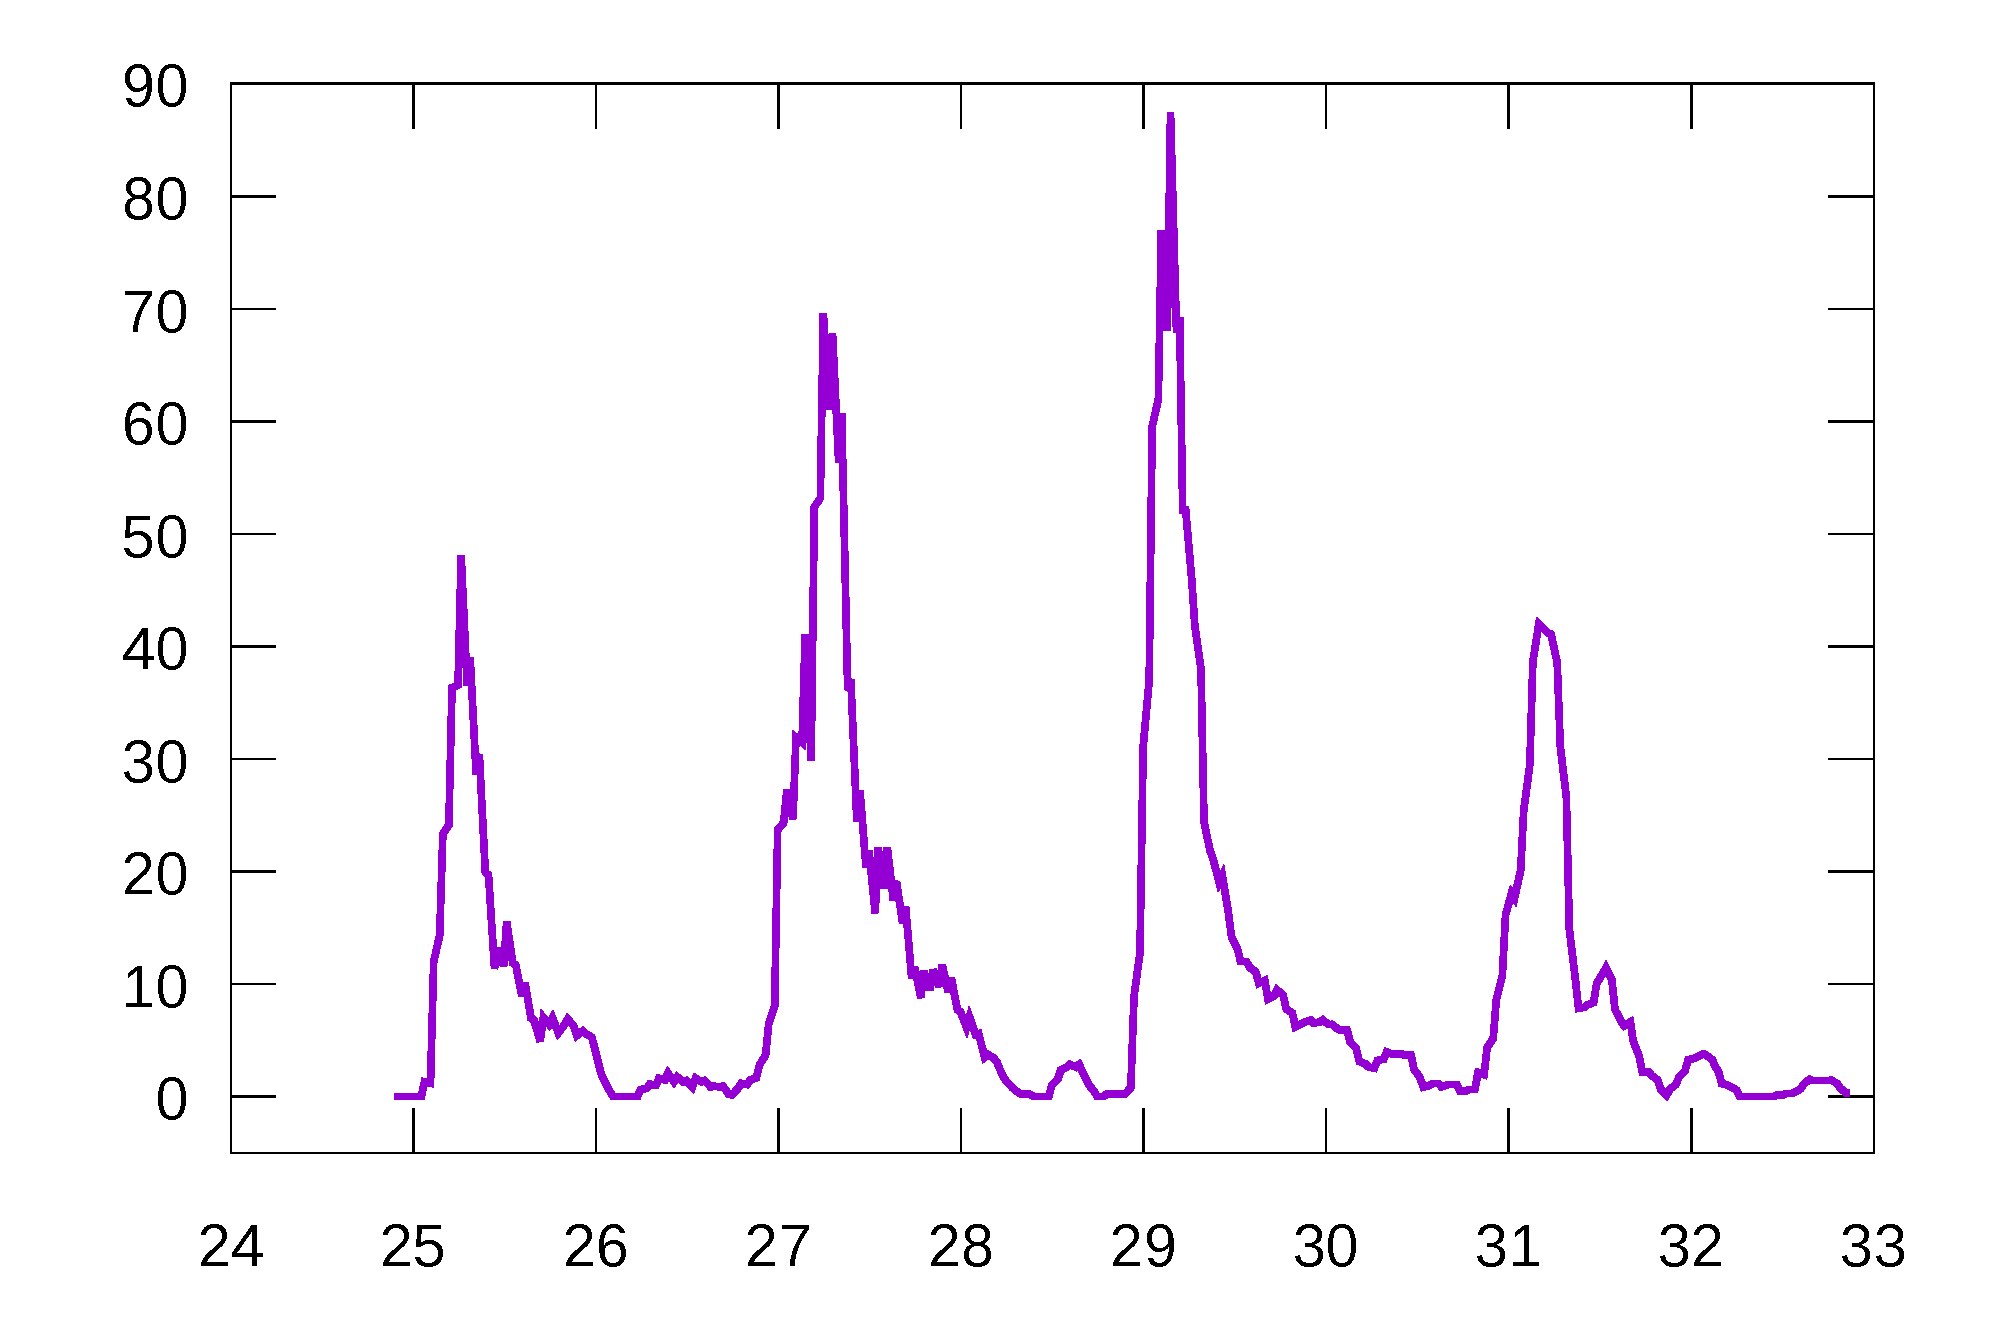
\includegraphics[width=\textwidth]{figures/ch4/subject_05_static_condition_smoothed}
			\caption{Profil du sujet 5.}
			\label{fig:staticProfile5}
		\end{subfigure}
		~
		\begin{subfigure}[t]{\subImgWlineplot}
			\centering
			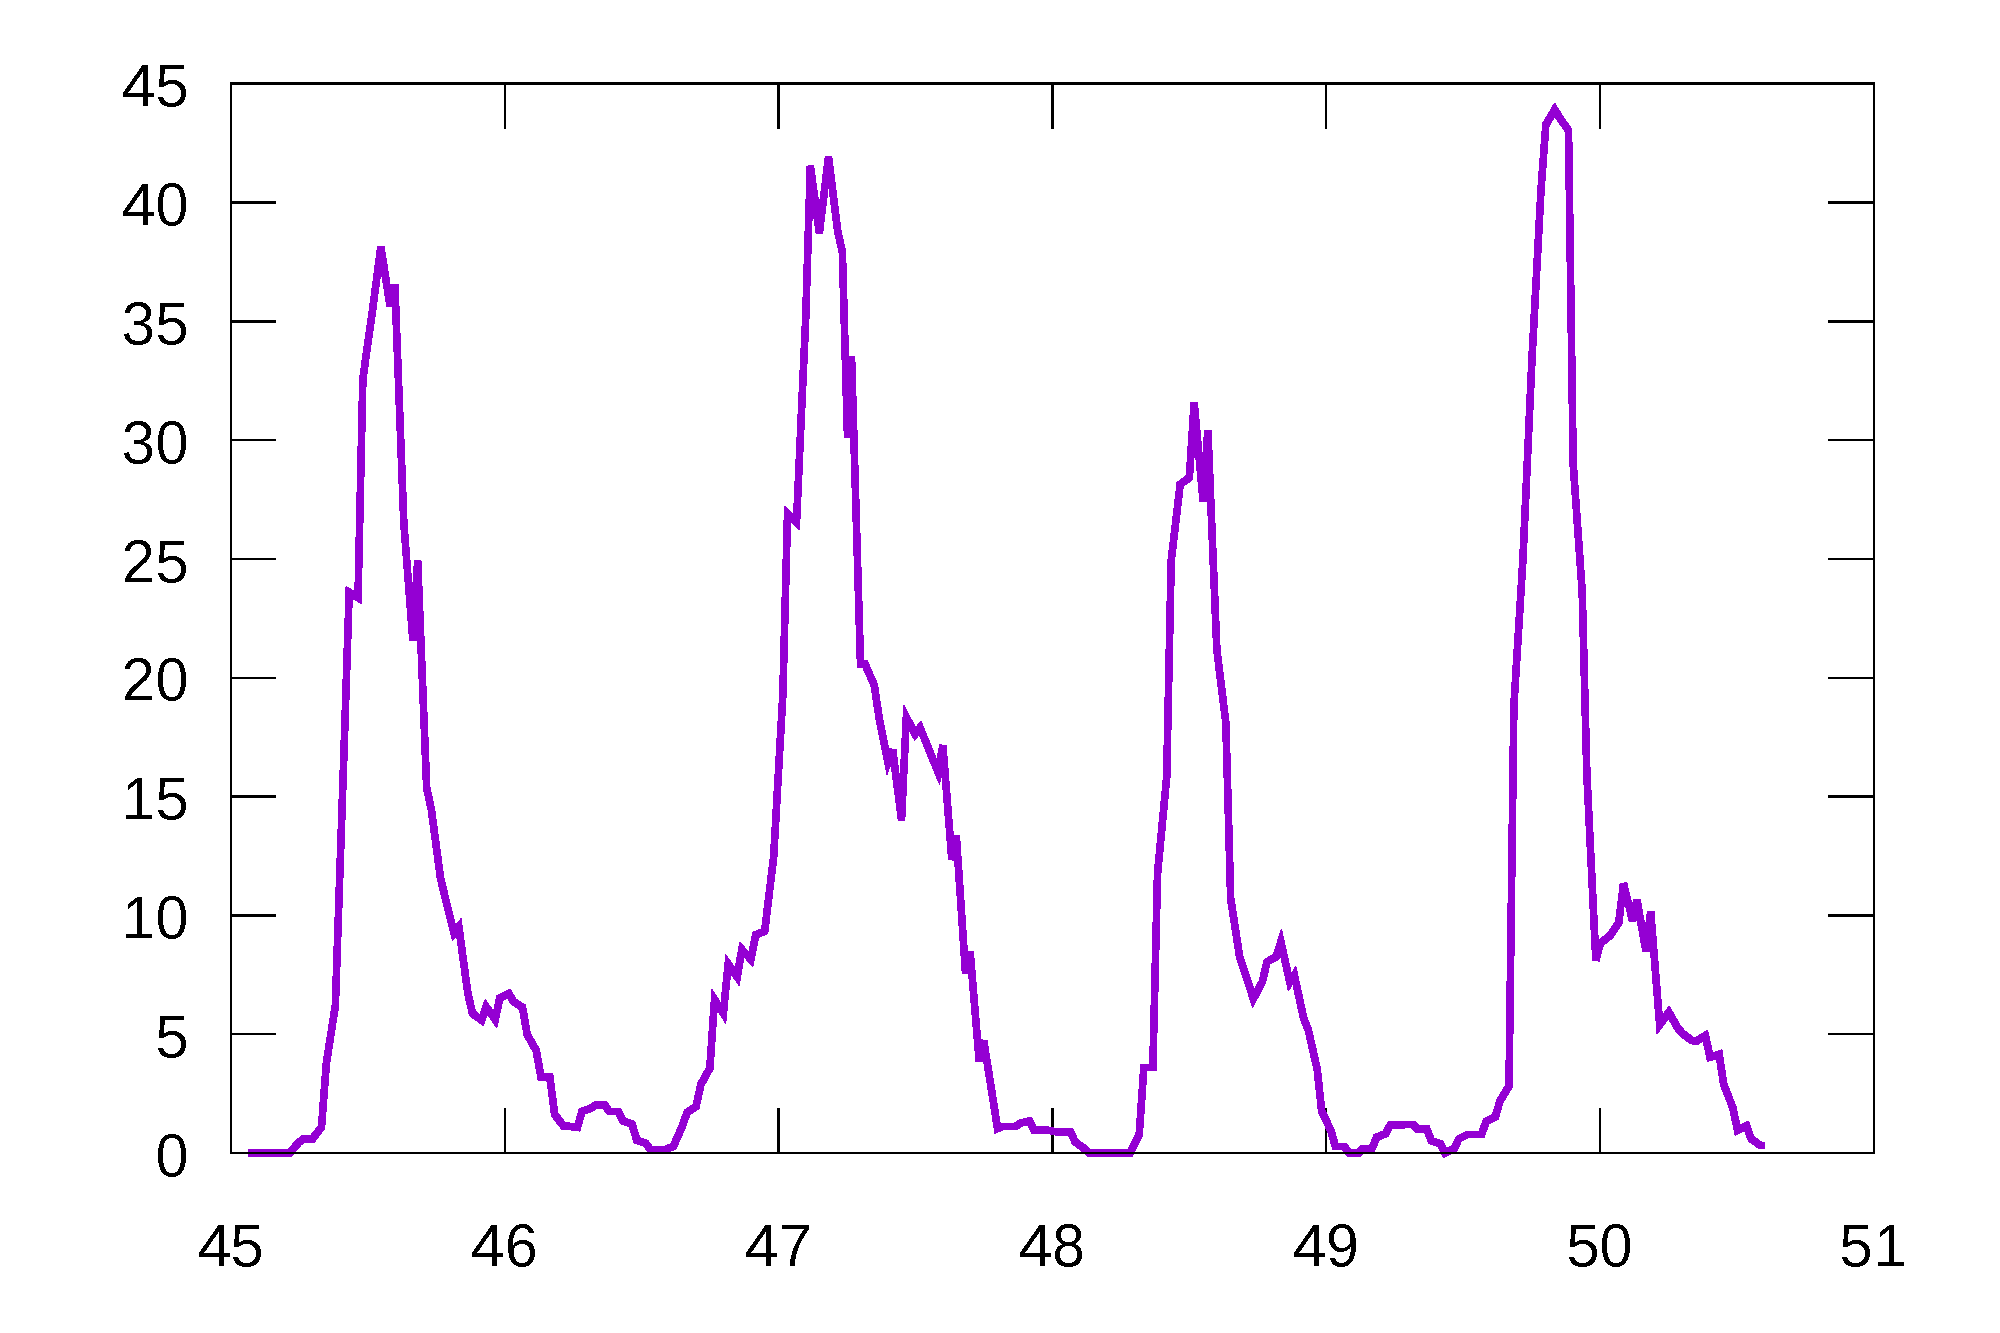
\includegraphics[width=\textwidth]{figures/ch4/subject_06_static_condition_smoothed}
			\caption{Profil du sujet 6.}
			\label{fig:staticProfile6}
		\end{subfigure}
		~
		\begin{subfigure}[t]{\subImgWlineplot}
			\centering
			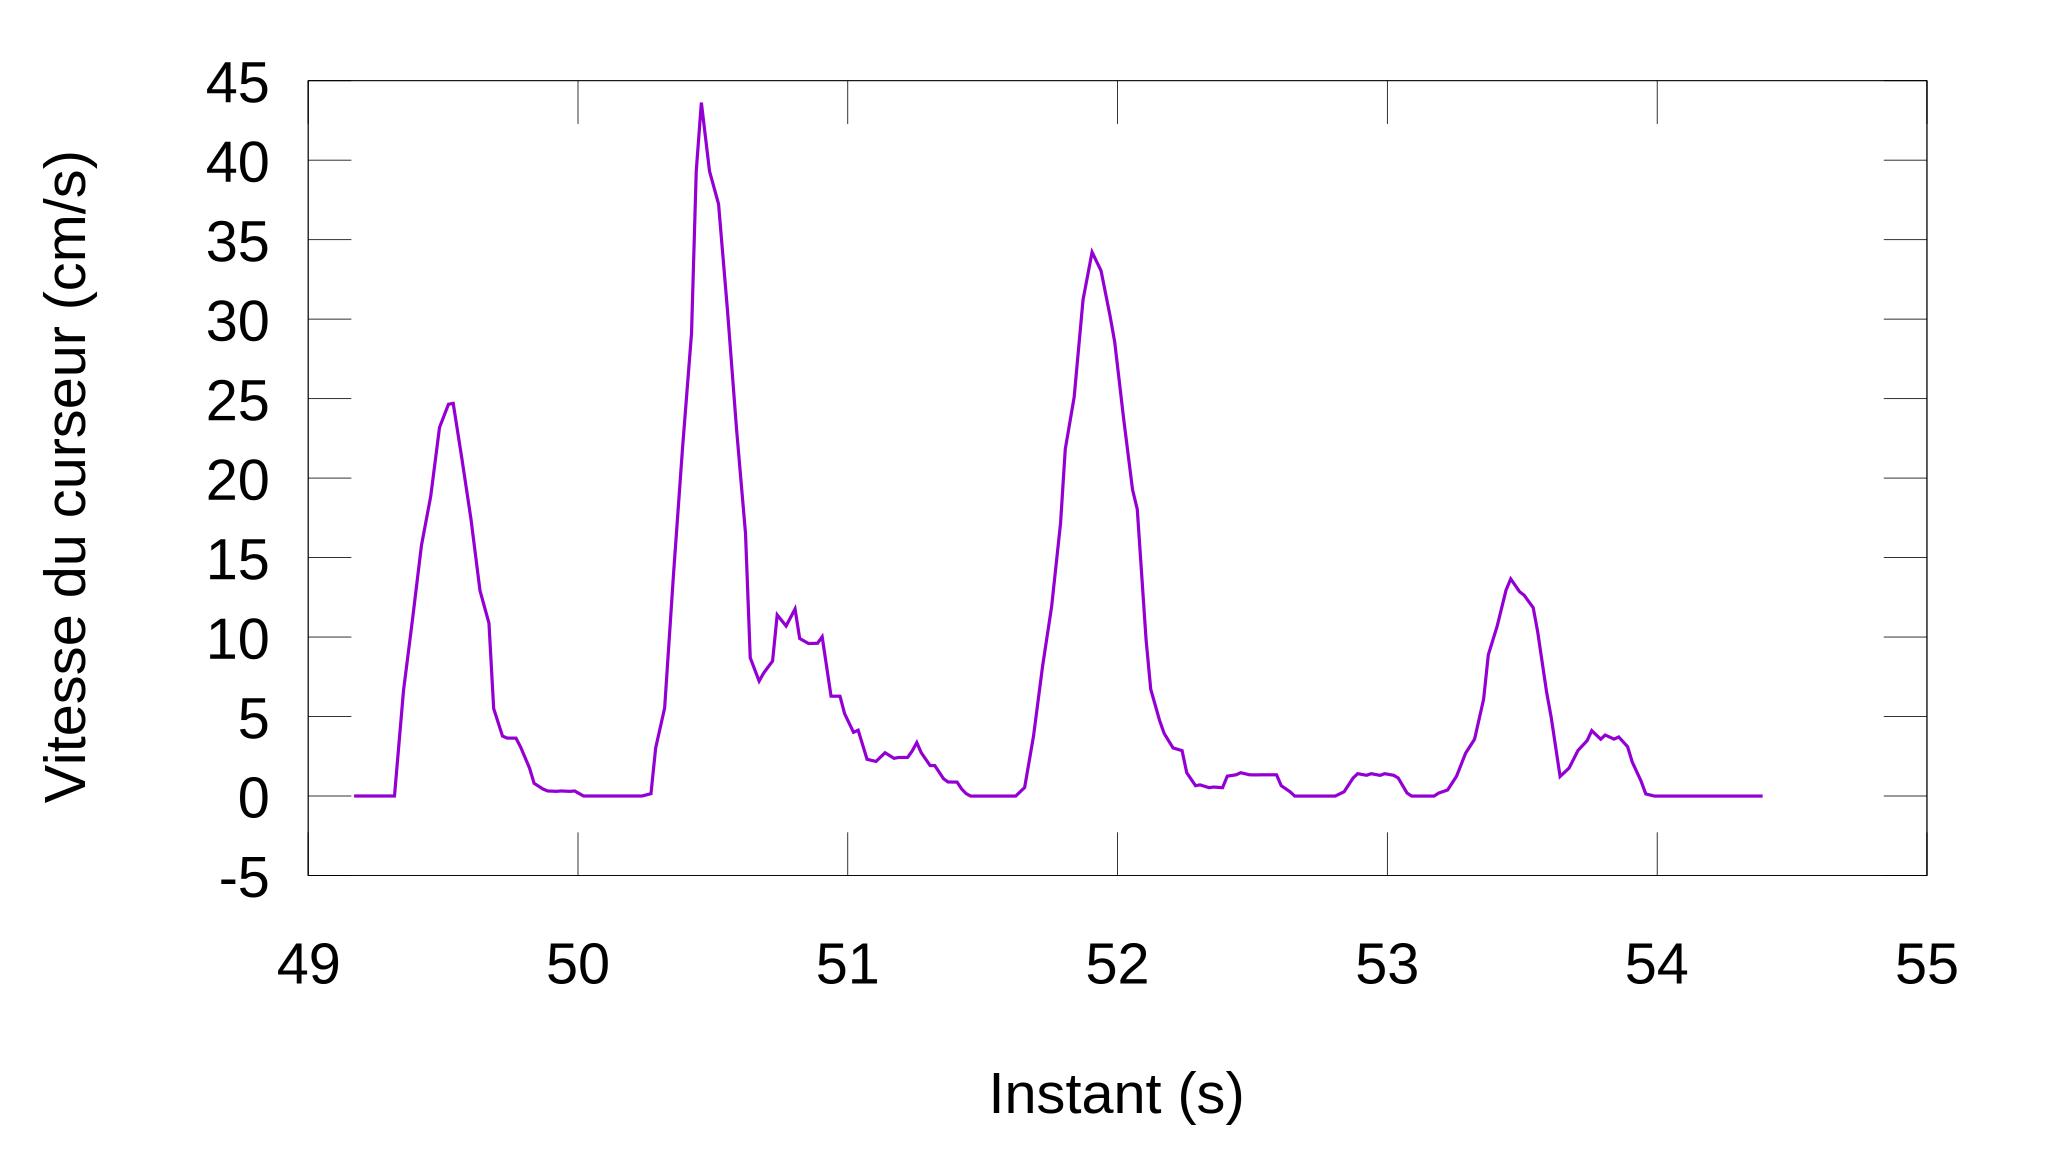
\includegraphics[width=\textwidth]{figures/ch4/subject_08_static_condition_smoothed}
			\caption{Profil du sujet 8.}
			\label{fig:staticProfile8}
		\end{subfigure}
		~
		\begin{subfigure}[t]{\subImgWlineplot}
			\centering
			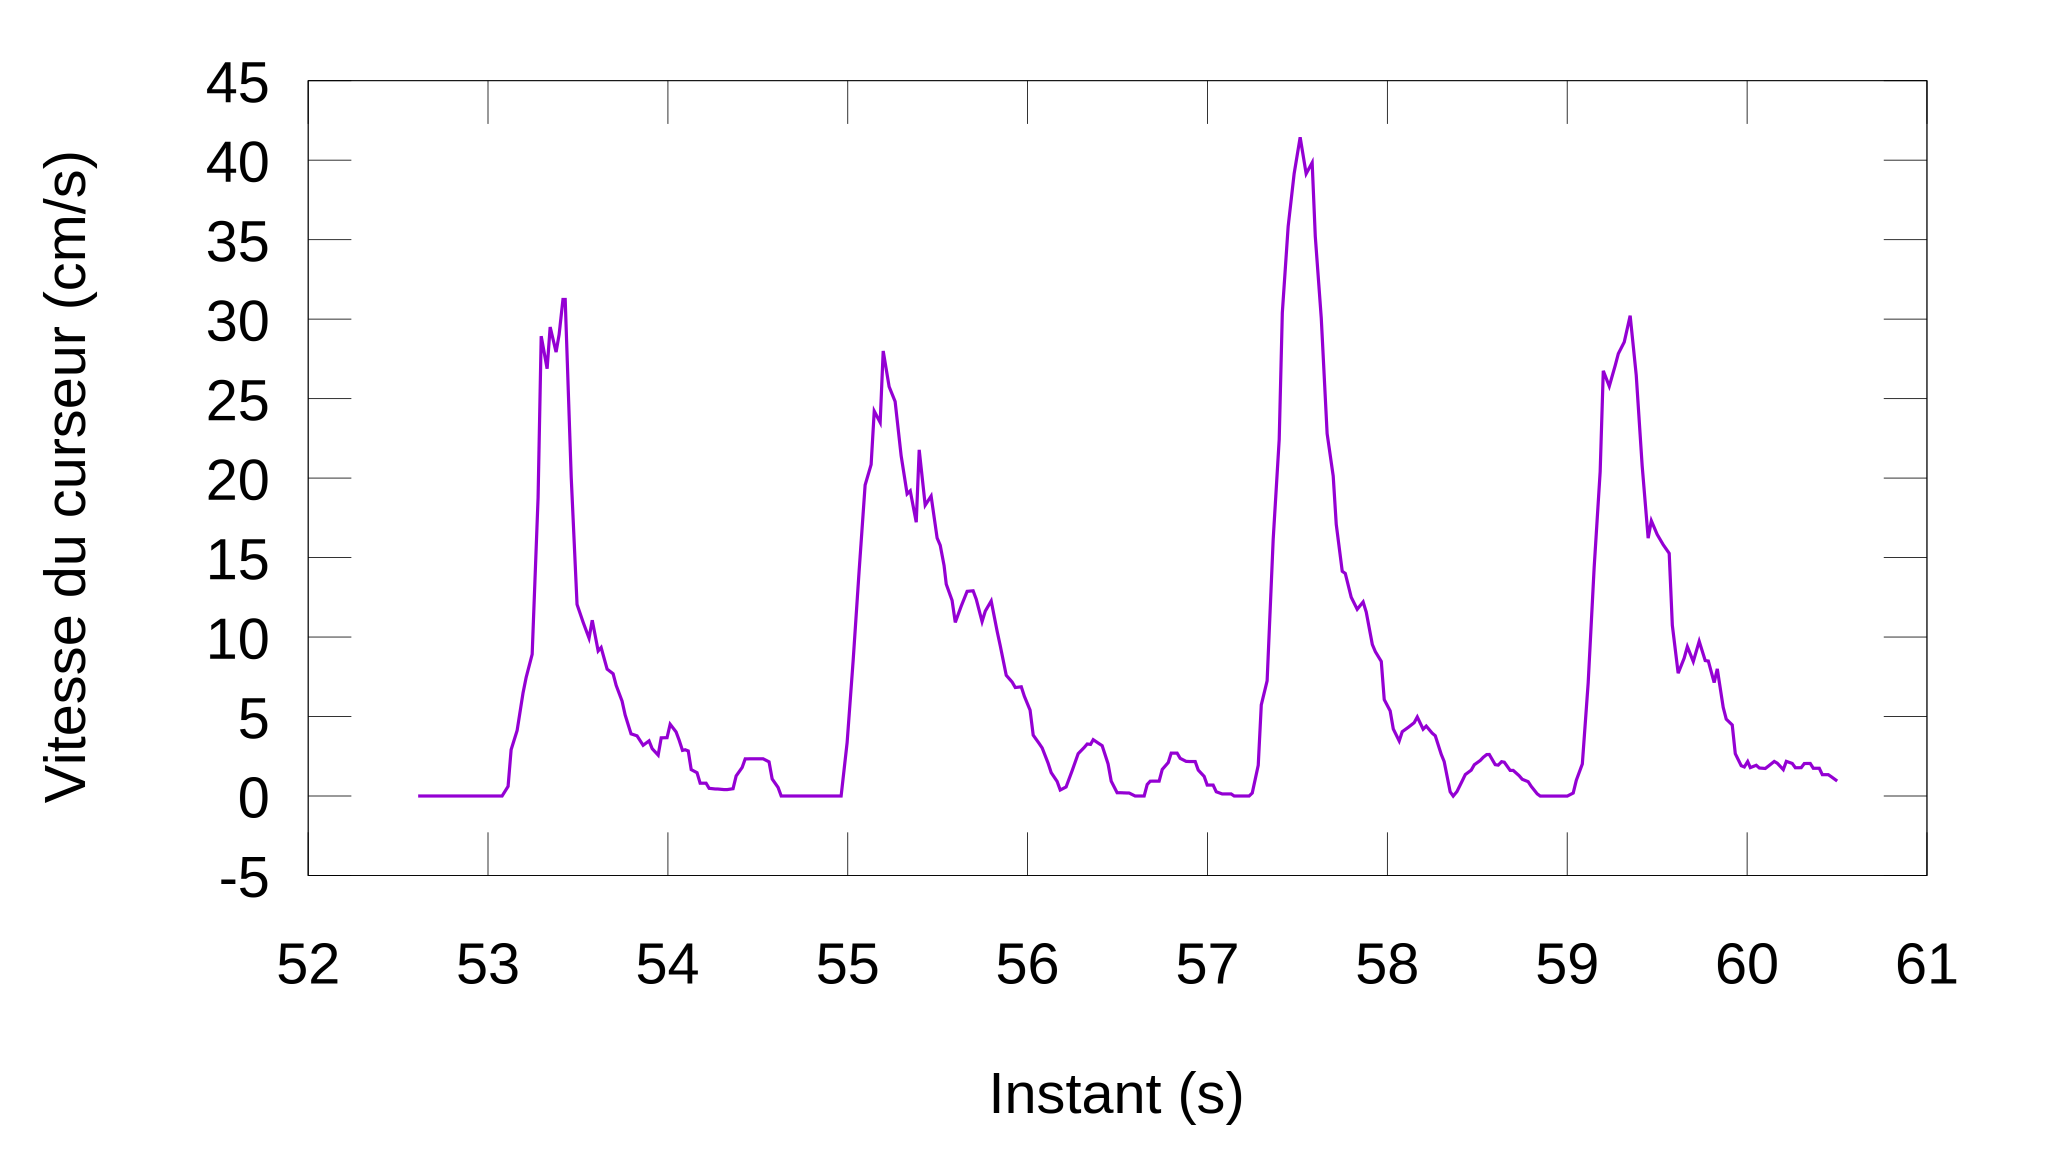
\includegraphics[width=\textwidth]{figures/ch4/subject_09_static_condition_smoothed}
			\caption{Profil du sujet 9.}
			\label{fig:staticProfile9}
		\end{subfigure}
		\caption[Profils de vitesse du curseur, cibles statiques]{Profils lissés de vitesse du curseur pour quatre sujets, avec des cibles statiques. Le temps (en secondes) est en abscisse et la vitesse (en cm/s) est en ordonnée.}
		\label{fig:staticProfiles}
	\end{figure}
	
	On constate sur ces profils que les phases balistiques et de correction sont relativement équilibrées, leurs part respectives du temps de sélection étant approximativement les mêmes. Précisions que la limite entre la phase balistique et la phase de correction n'est pas toujours délimitée de façon très précise, aussi est-il difficile d'en faire des mesures exactes. Mais il est possible de tirer des enseignements d'un examen visuel des profils, ainsi que de mesures quantitatives et précises de la vitesse du curseur.
	
	\subsubsection{Cibles en mouvement rectiligne}
	Si l'on compare les profils de la figure~\ref{fig:staticProfiles}, enregistrés pendant des sélections de cibles statiques, à ceux de la figure~\ref{fig:rectProfiles}, issus de sélections de cibles de mouvement rectiligne, on remarque déjà des différences, alors que le mouvement rectiligne est celui qui génère le moins de difficultés. On observe en effet que les sélections sont plus longues, mais que la durée des phases balistiques n'est pas sensiblement modifiée. En revanche, les phases de correction sont rallongées, et leur forme change quelque peu, avec l'apparition d'oscillations dont l'amplitude peut atteindre --- voire dépasser --- les 10~cm/s.
	
	\begin{figure}[!htb]
		\centering
		\begin{subfigure}[t]{\subImgWlineplot}
			\centering
			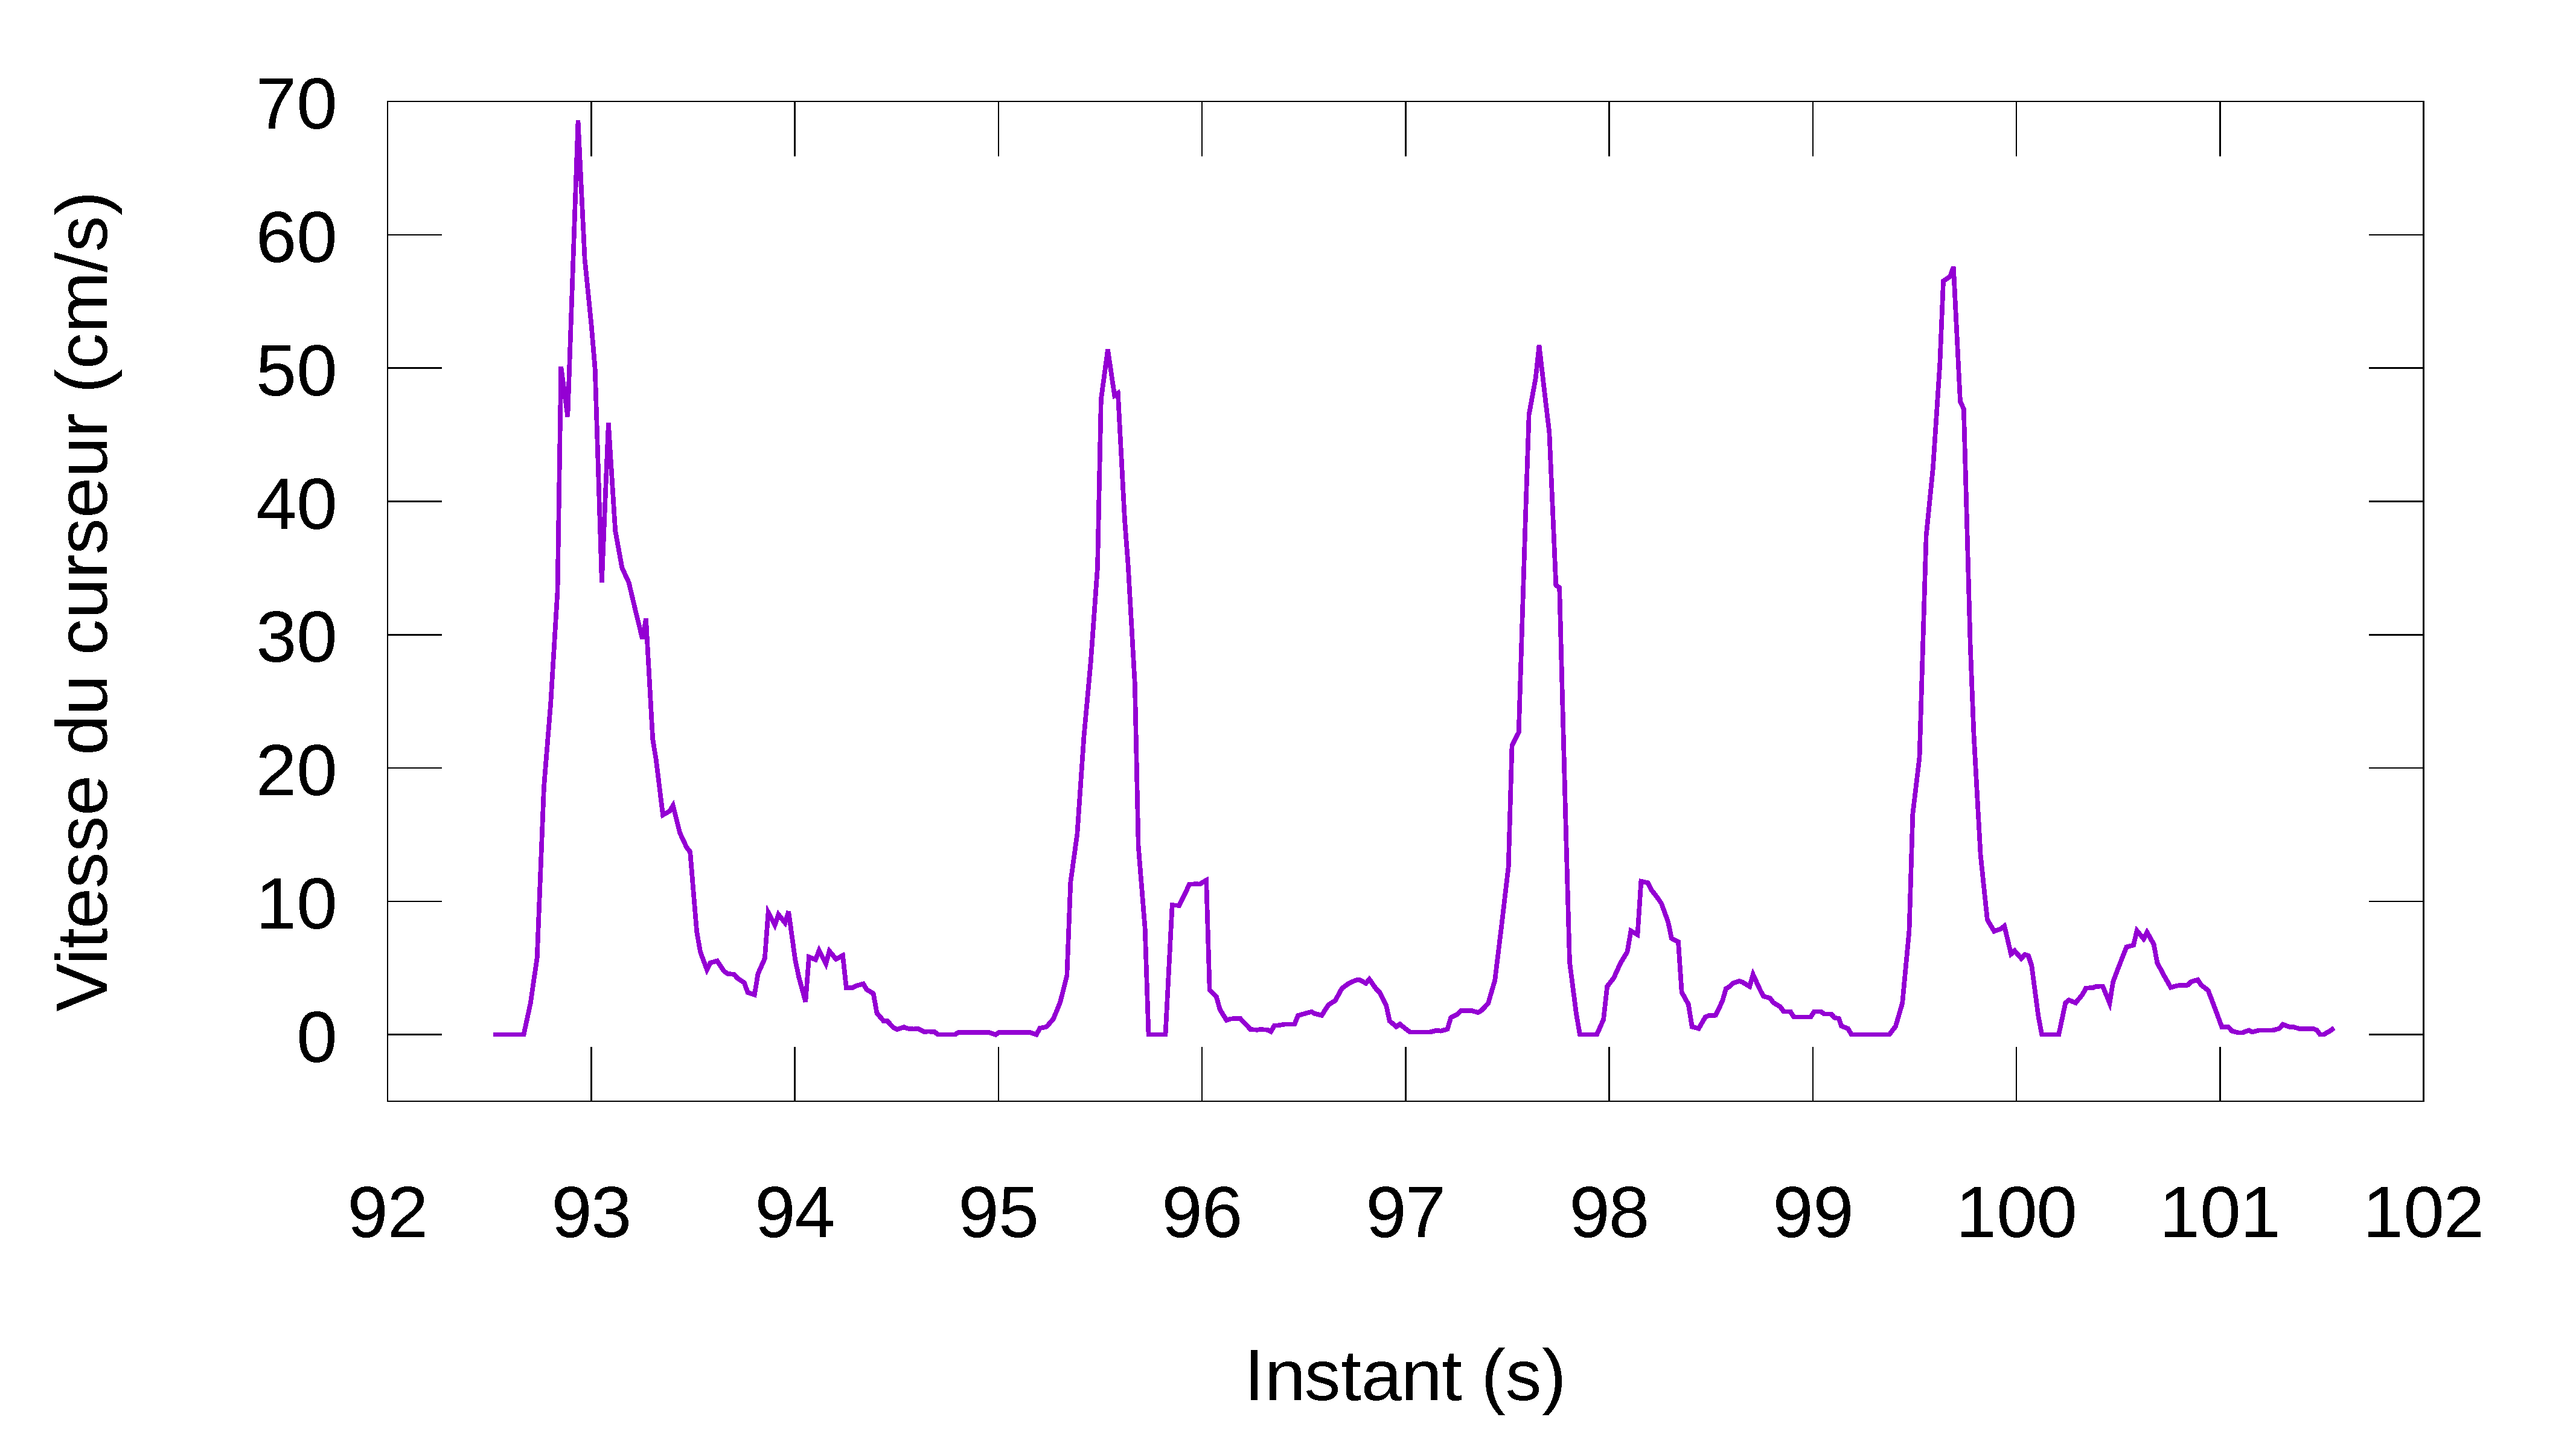
\includegraphics[width=\textwidth]{figures/ch4/subject_05_rect_219_smoothed}
			\caption{Profil du sujet 5.}
			\label{fig:rectProfile5}
		\end{subfigure}
		~
		\begin{subfigure}[t]{\subImgWlineplot}
			\centering
			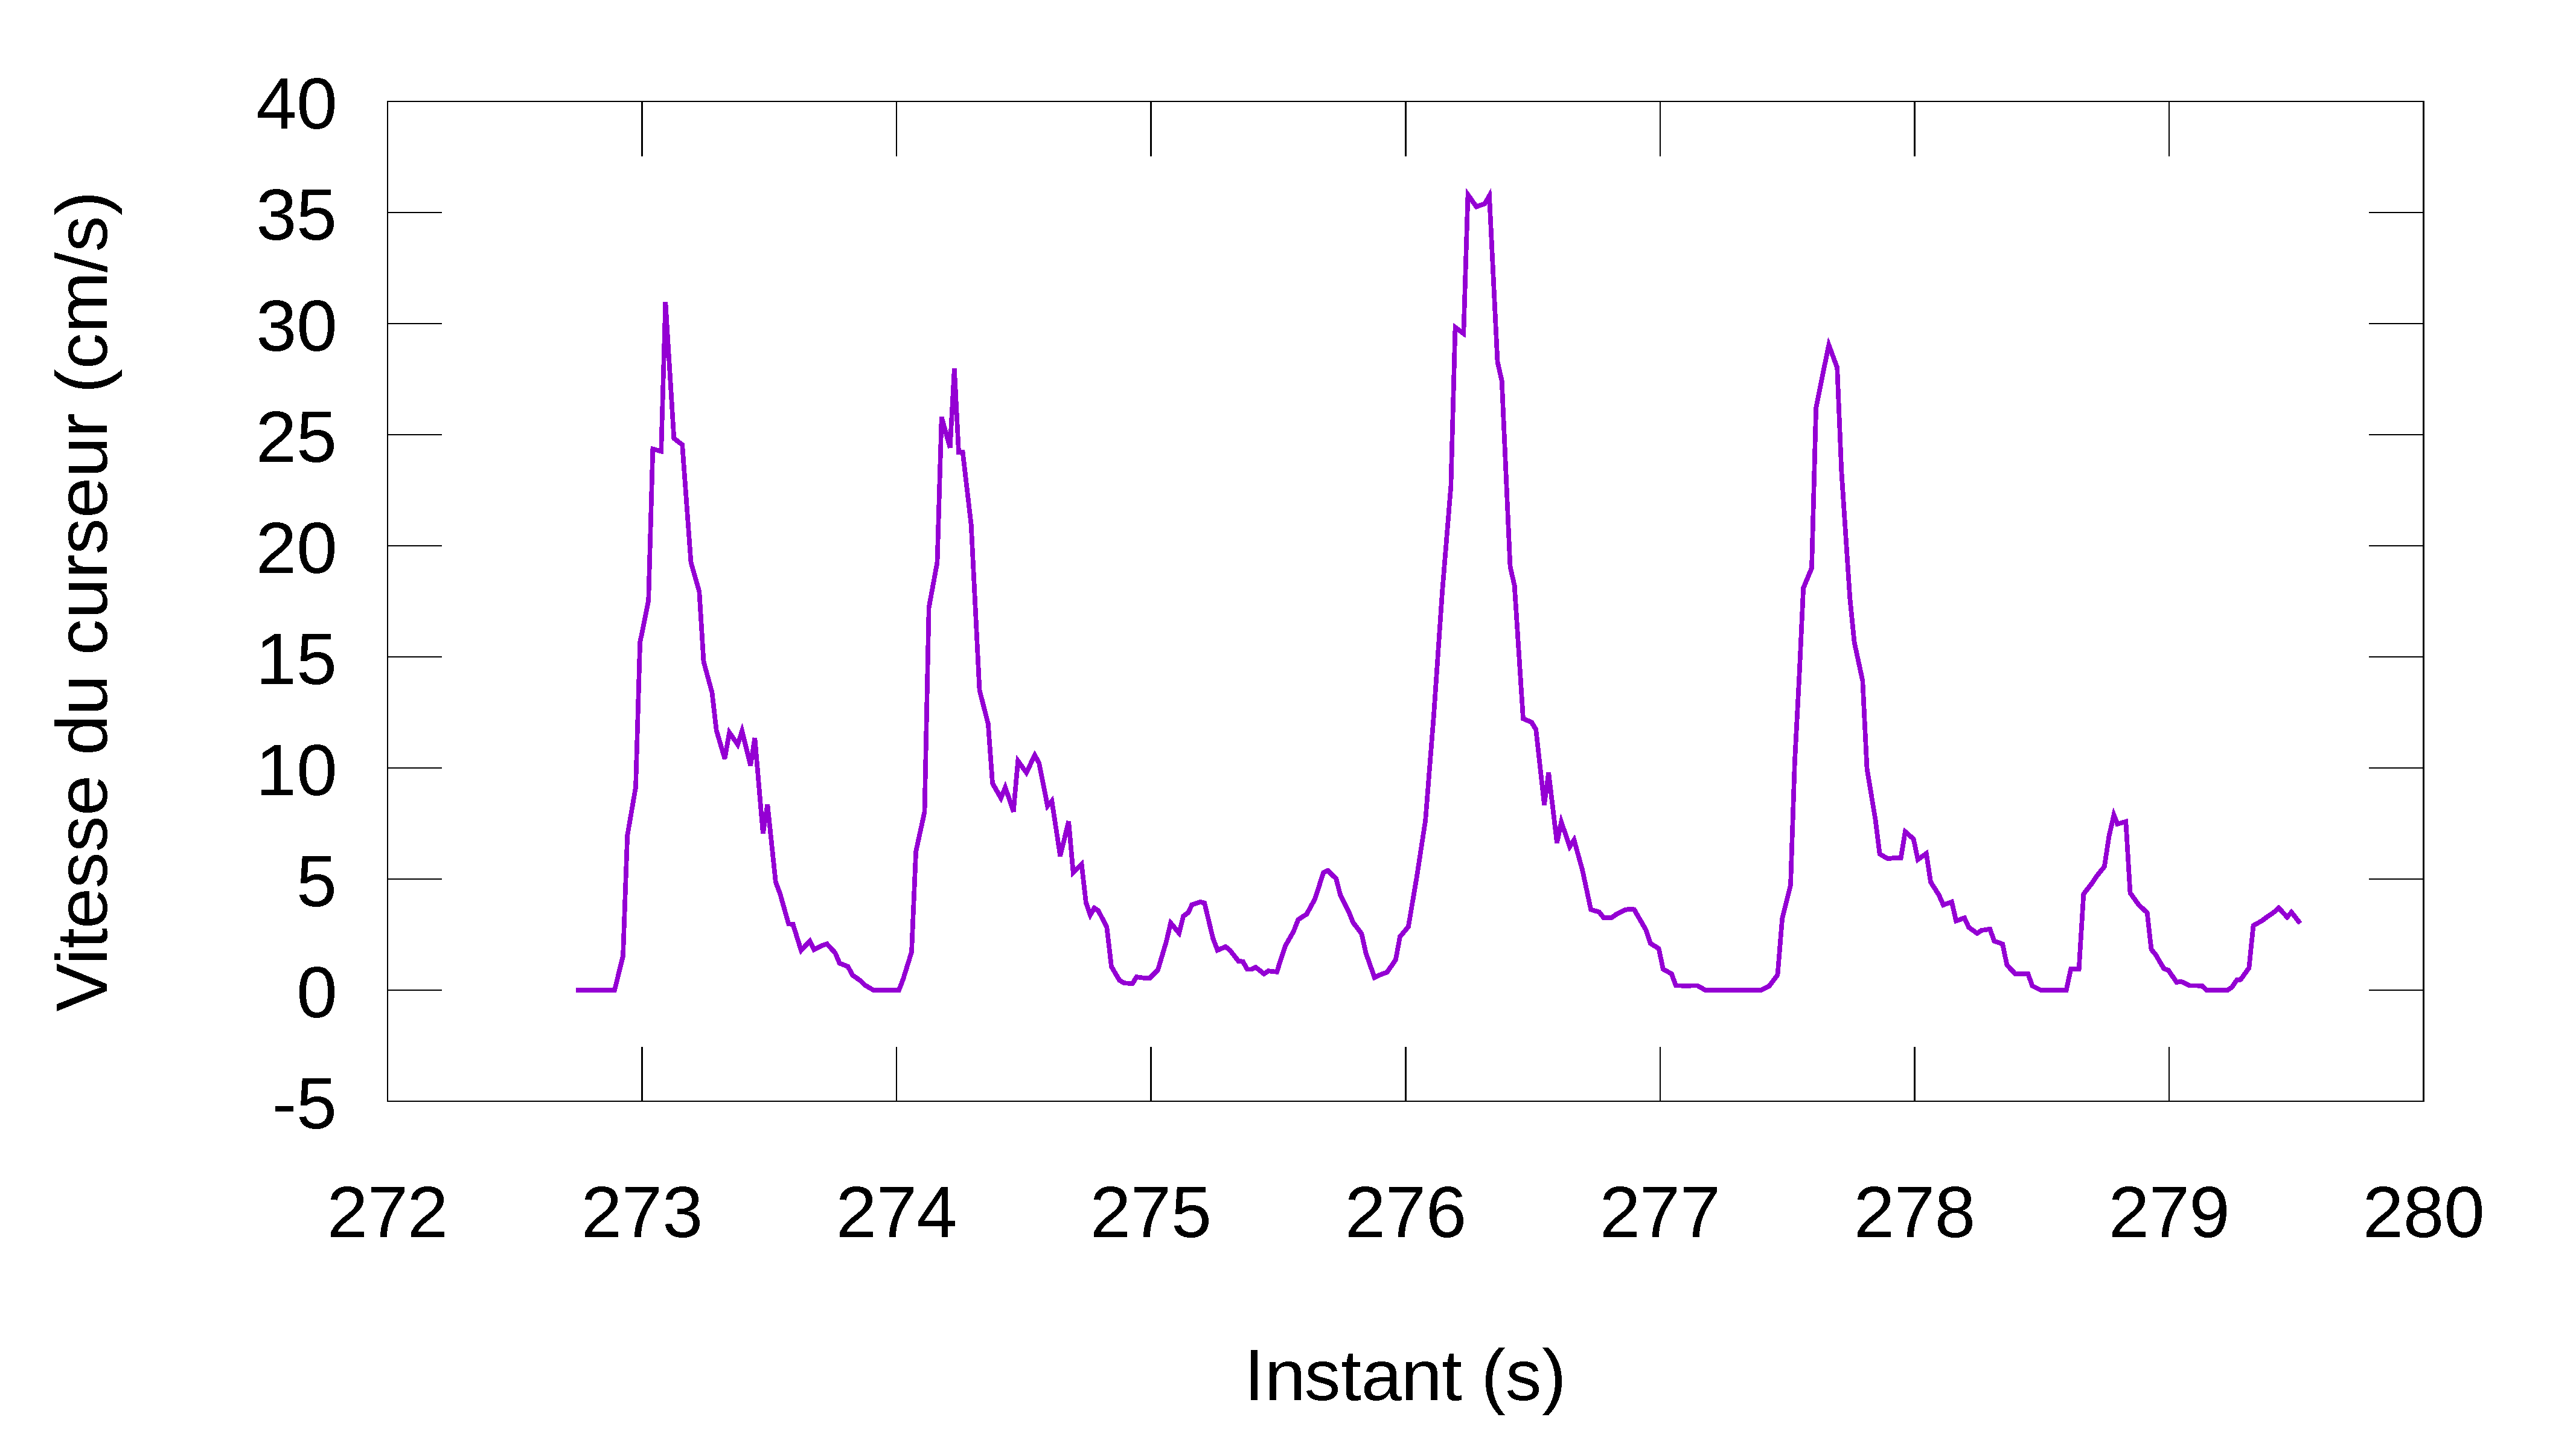
\includegraphics[width=\textwidth]{figures/ch4/subject_06_rect_219_smoothed}
			\caption{Profil du sujet 6.}
			\label{fig:rectProfile6}
		\end{subfigure}
		~
		\begin{subfigure}[t]{\subImgWlineplot}
			\centering
			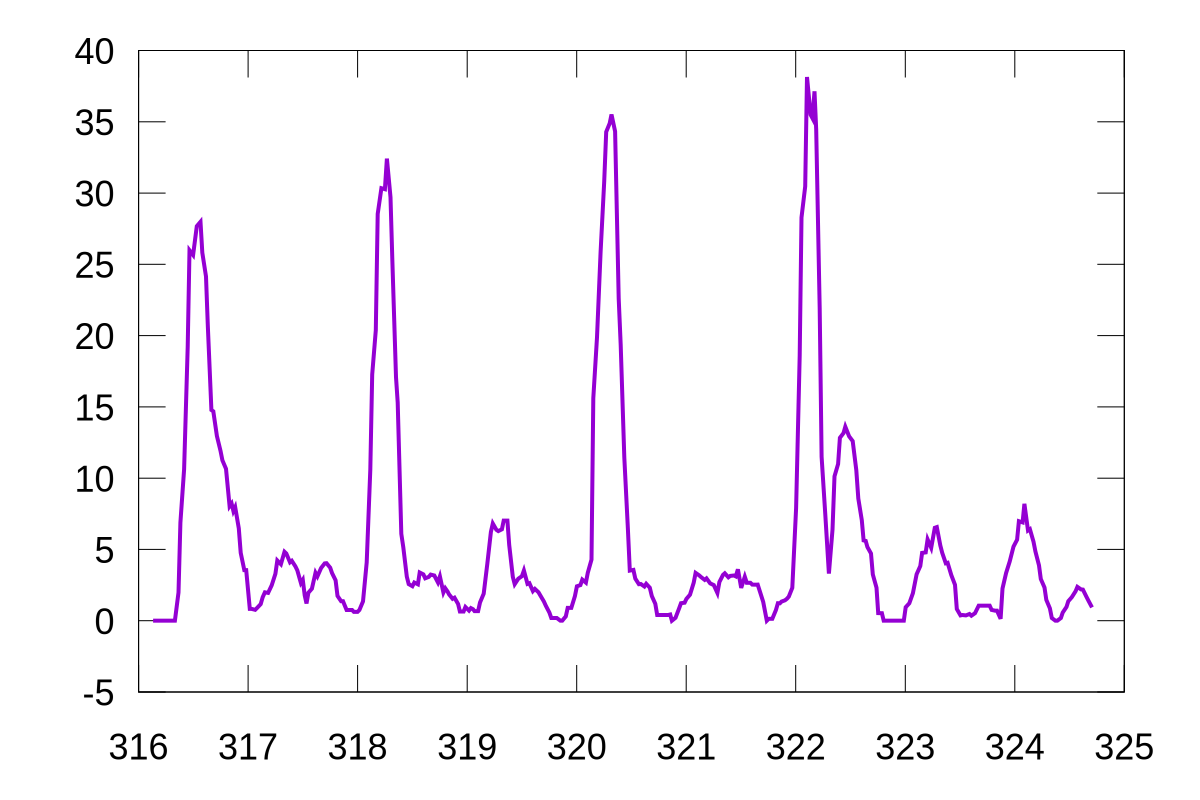
\includegraphics[width=\textwidth]{figures/ch4/subject_08_rect_219_smoothed}
			\caption{Profil du sujet 8.}
			\label{fig:rectProfile8}
		\end{subfigure}
		~
		\begin{subfigure}[t]{\subImgWlineplot}
			\centering
			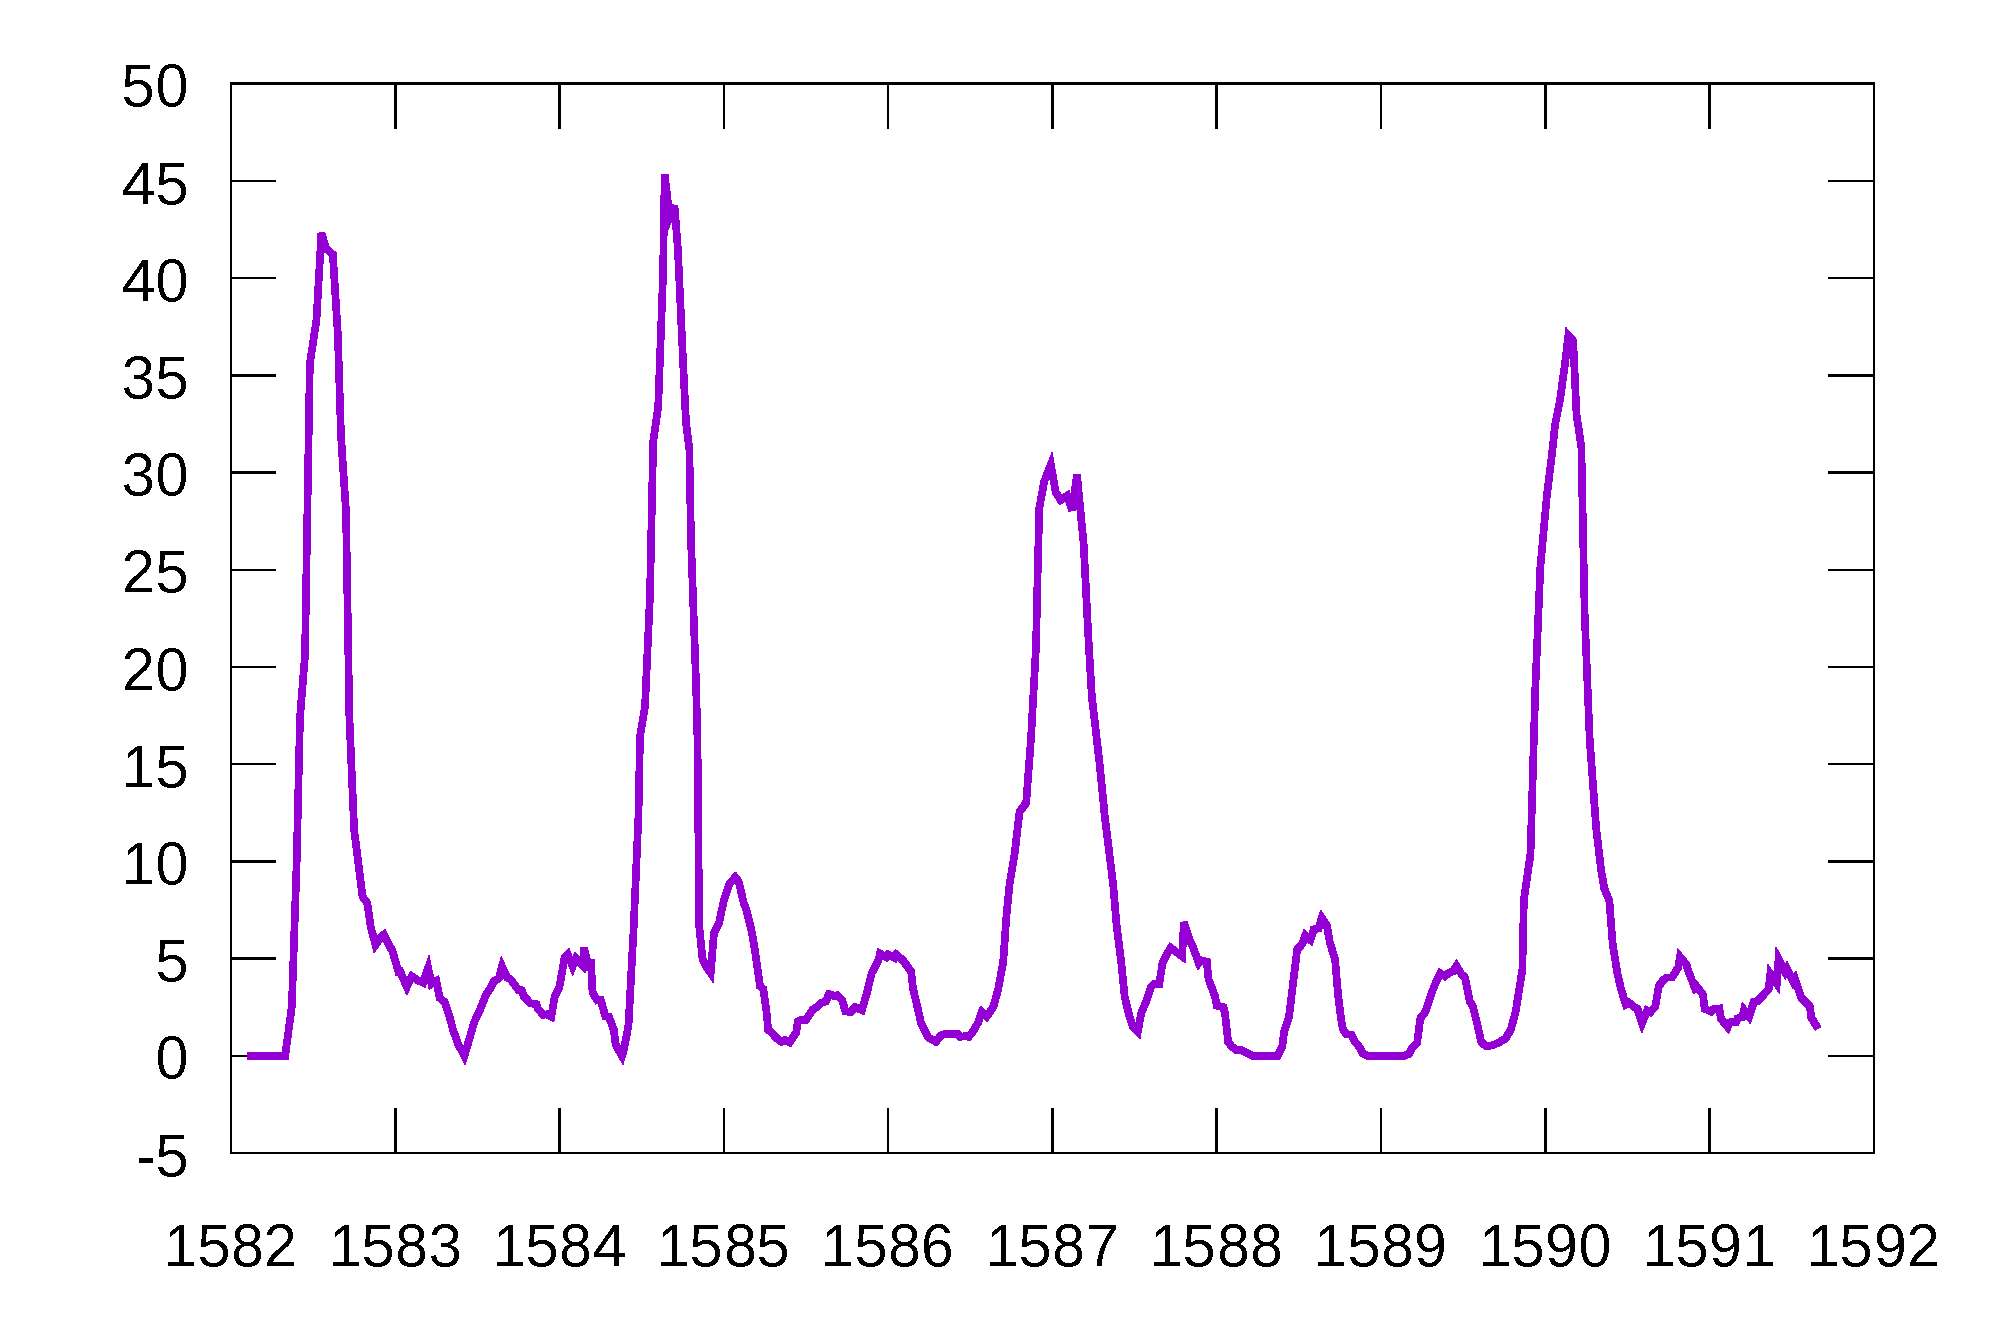
\includegraphics[width=\textwidth]{figures/ch4/subject_09_rect_219_smoothed}
			\caption{Profil du sujet 9.}
			\label{fig:rectProfile9}
		\end{subfigure}
		\caption[Profils de vitesse du curseur, cibles de mouvement rectiligne]{Profils lissés de vitesse du curseur pour quatre sujets, avec des cibles de mouvement rectiligne à 2,19~cm/s. Le temps (en secondes) est en abscisse et la vitesse (en cm/s) est en ordonnée.}
		\label{fig:rectProfiles}
	\end{figure}
	
	Si l'on examine les vitesses moyennes des curseurs de nos sujets lorsqu'ils sélectionnaient des cibles statiques d'une part, et en mouvement rectiligne d'autre part, l'on peut en effet remarquer que la vitesse moyenne du curseur chute légèrement lorsque les cibles sont mobiles ; ces données sont rapportées dans la table~\ref{tab:cursorSpeed}.
	
	C'est cependant moins vrai pour le sujet numéro 8, dont le curseur était en moyenne à peine moins rapide avec des cibles en mouvement rectiligne. Pourtant, l'examen de ses profils de vitesse montre que les phases de correction étaient nettement plus longues avec des cibles en mouvement rectiligne. La raison de cette légère anomalie est très probablement la faible vitesse moyenne de son curseur lors de la sélection de cibles statiques, qui s'explique sans doute par la faible hauteur des \og pics \fg{} de ses phases balistiques avec des cibles statiques. Peut-être la facilité perçue de la tâche n'encourageait-elle pas suffisamment ce sujet à se presser quand les cibles étaient statiques.
	
	\begin{table}
		\centering
		\begin{tabular}{c | c c | c}
						& \multicolumn{2}{c |}{Vitesses moyennes}	&							\bigstrut[b] \\
			Sujet		& Cible statique	& Mouvement rectiligne	& Différence de pourcentage	\bigstrut[b] \\ \hline
			5			& 11,10~cm/s		& 8,00~cm/s				& 32,44~\%{}				\bigstrut[t] \\
			6			& 9,82~cm/s			& 8,57~cm/s				& 13,60~\%{}				\\
			8			& 7,65~cm/s			& 7,05~cm/s				& 8,13~\%{}					\\
			9			& 8,48~cm/s			& 6,46~cm/s				& 26,98~\%{}				\\
		\end{tabular}
		\caption[Vitesses moyennes du curseur, cibles statiques ou en mouvement rectiligne]{Vitesses moyennes (en cm/s) du curseur pour quatre sujets différents, au cours de sélections de cibles statiques d'une part, en mouvement rectiligne d'autre part. Les différences de pourcentages entre les deux conditions sont présentées dans la quatrième colonne.}
		\label{tab:cursorSpeed}
	\end{table}
	
	\subsubsection{Cibles aux mouvements imprévisibles}
	Les choses deviennent beaucoup plus nettes lorsque l'on s'intéresse aux conditions les plus difficiles. Comme on le voit sur la figure~\ref{fig:hardProfiles}, les phases balistiques sont réduites à de courts sursauts de vitesse, et les phases de correction dominent largement le temps total de sélection. Bien sûr, ce n'est pas dû à une réduction de la durée des phases balistiques, mais à un rallongement des phases de correction.

	\begin{figure}[!htb]
		\centering
		\begin{subfigure}[t]{\subImgWlineplot}
			\centering
			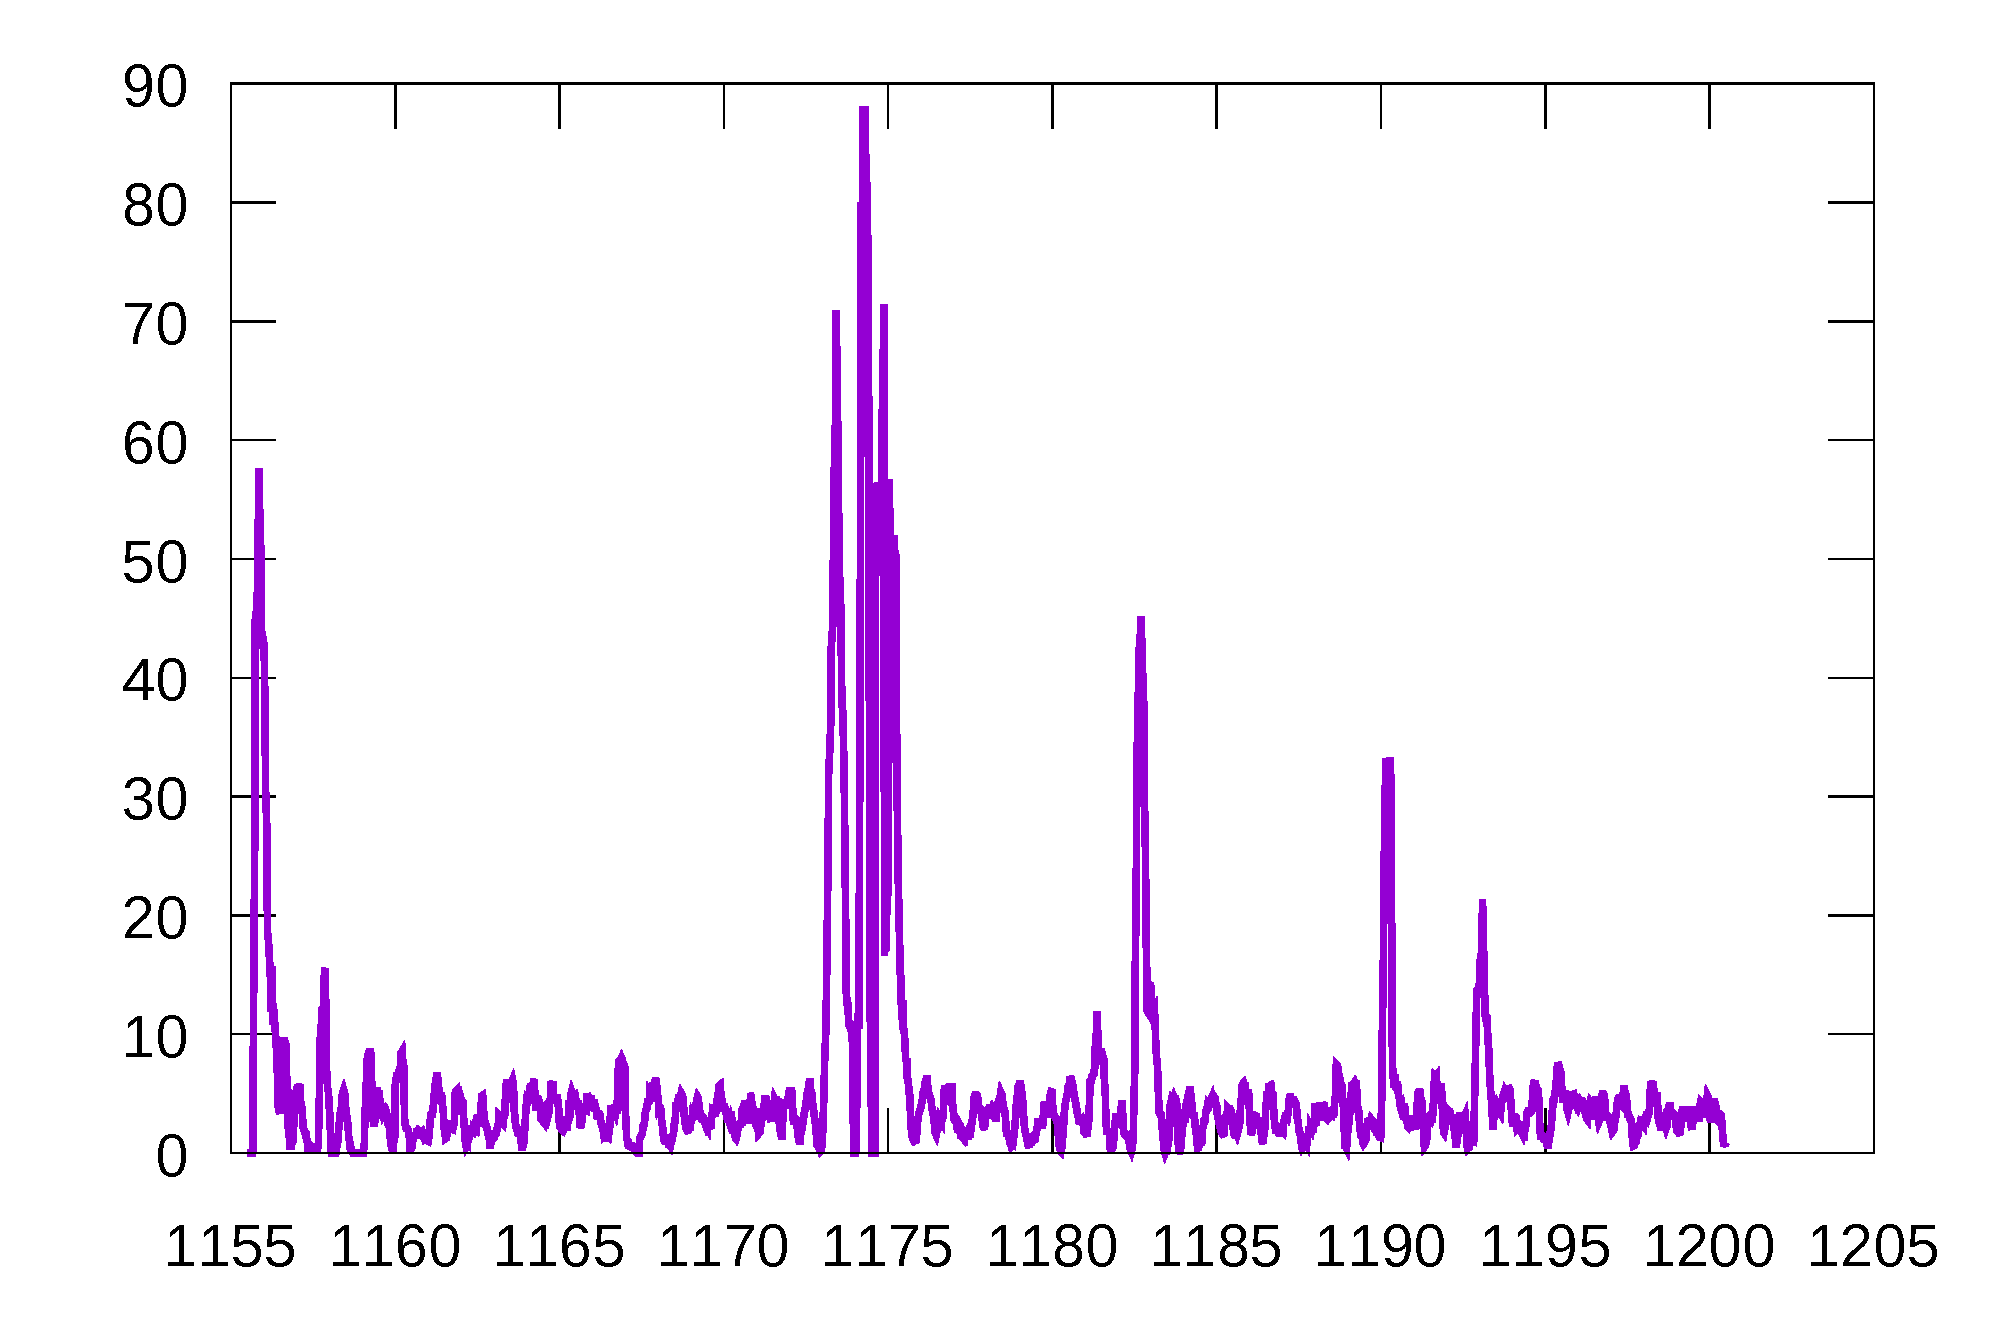
\includegraphics[width=\textwidth]{figures/ch4/subject_05_60_8_219_smoothed}
			\caption{Profil du sujet 5.}
			\label{fig:hardProfile5}
		\end{subfigure}
		~
		\begin{subfigure}[t]{\subImgWlineplot}
			\centering
			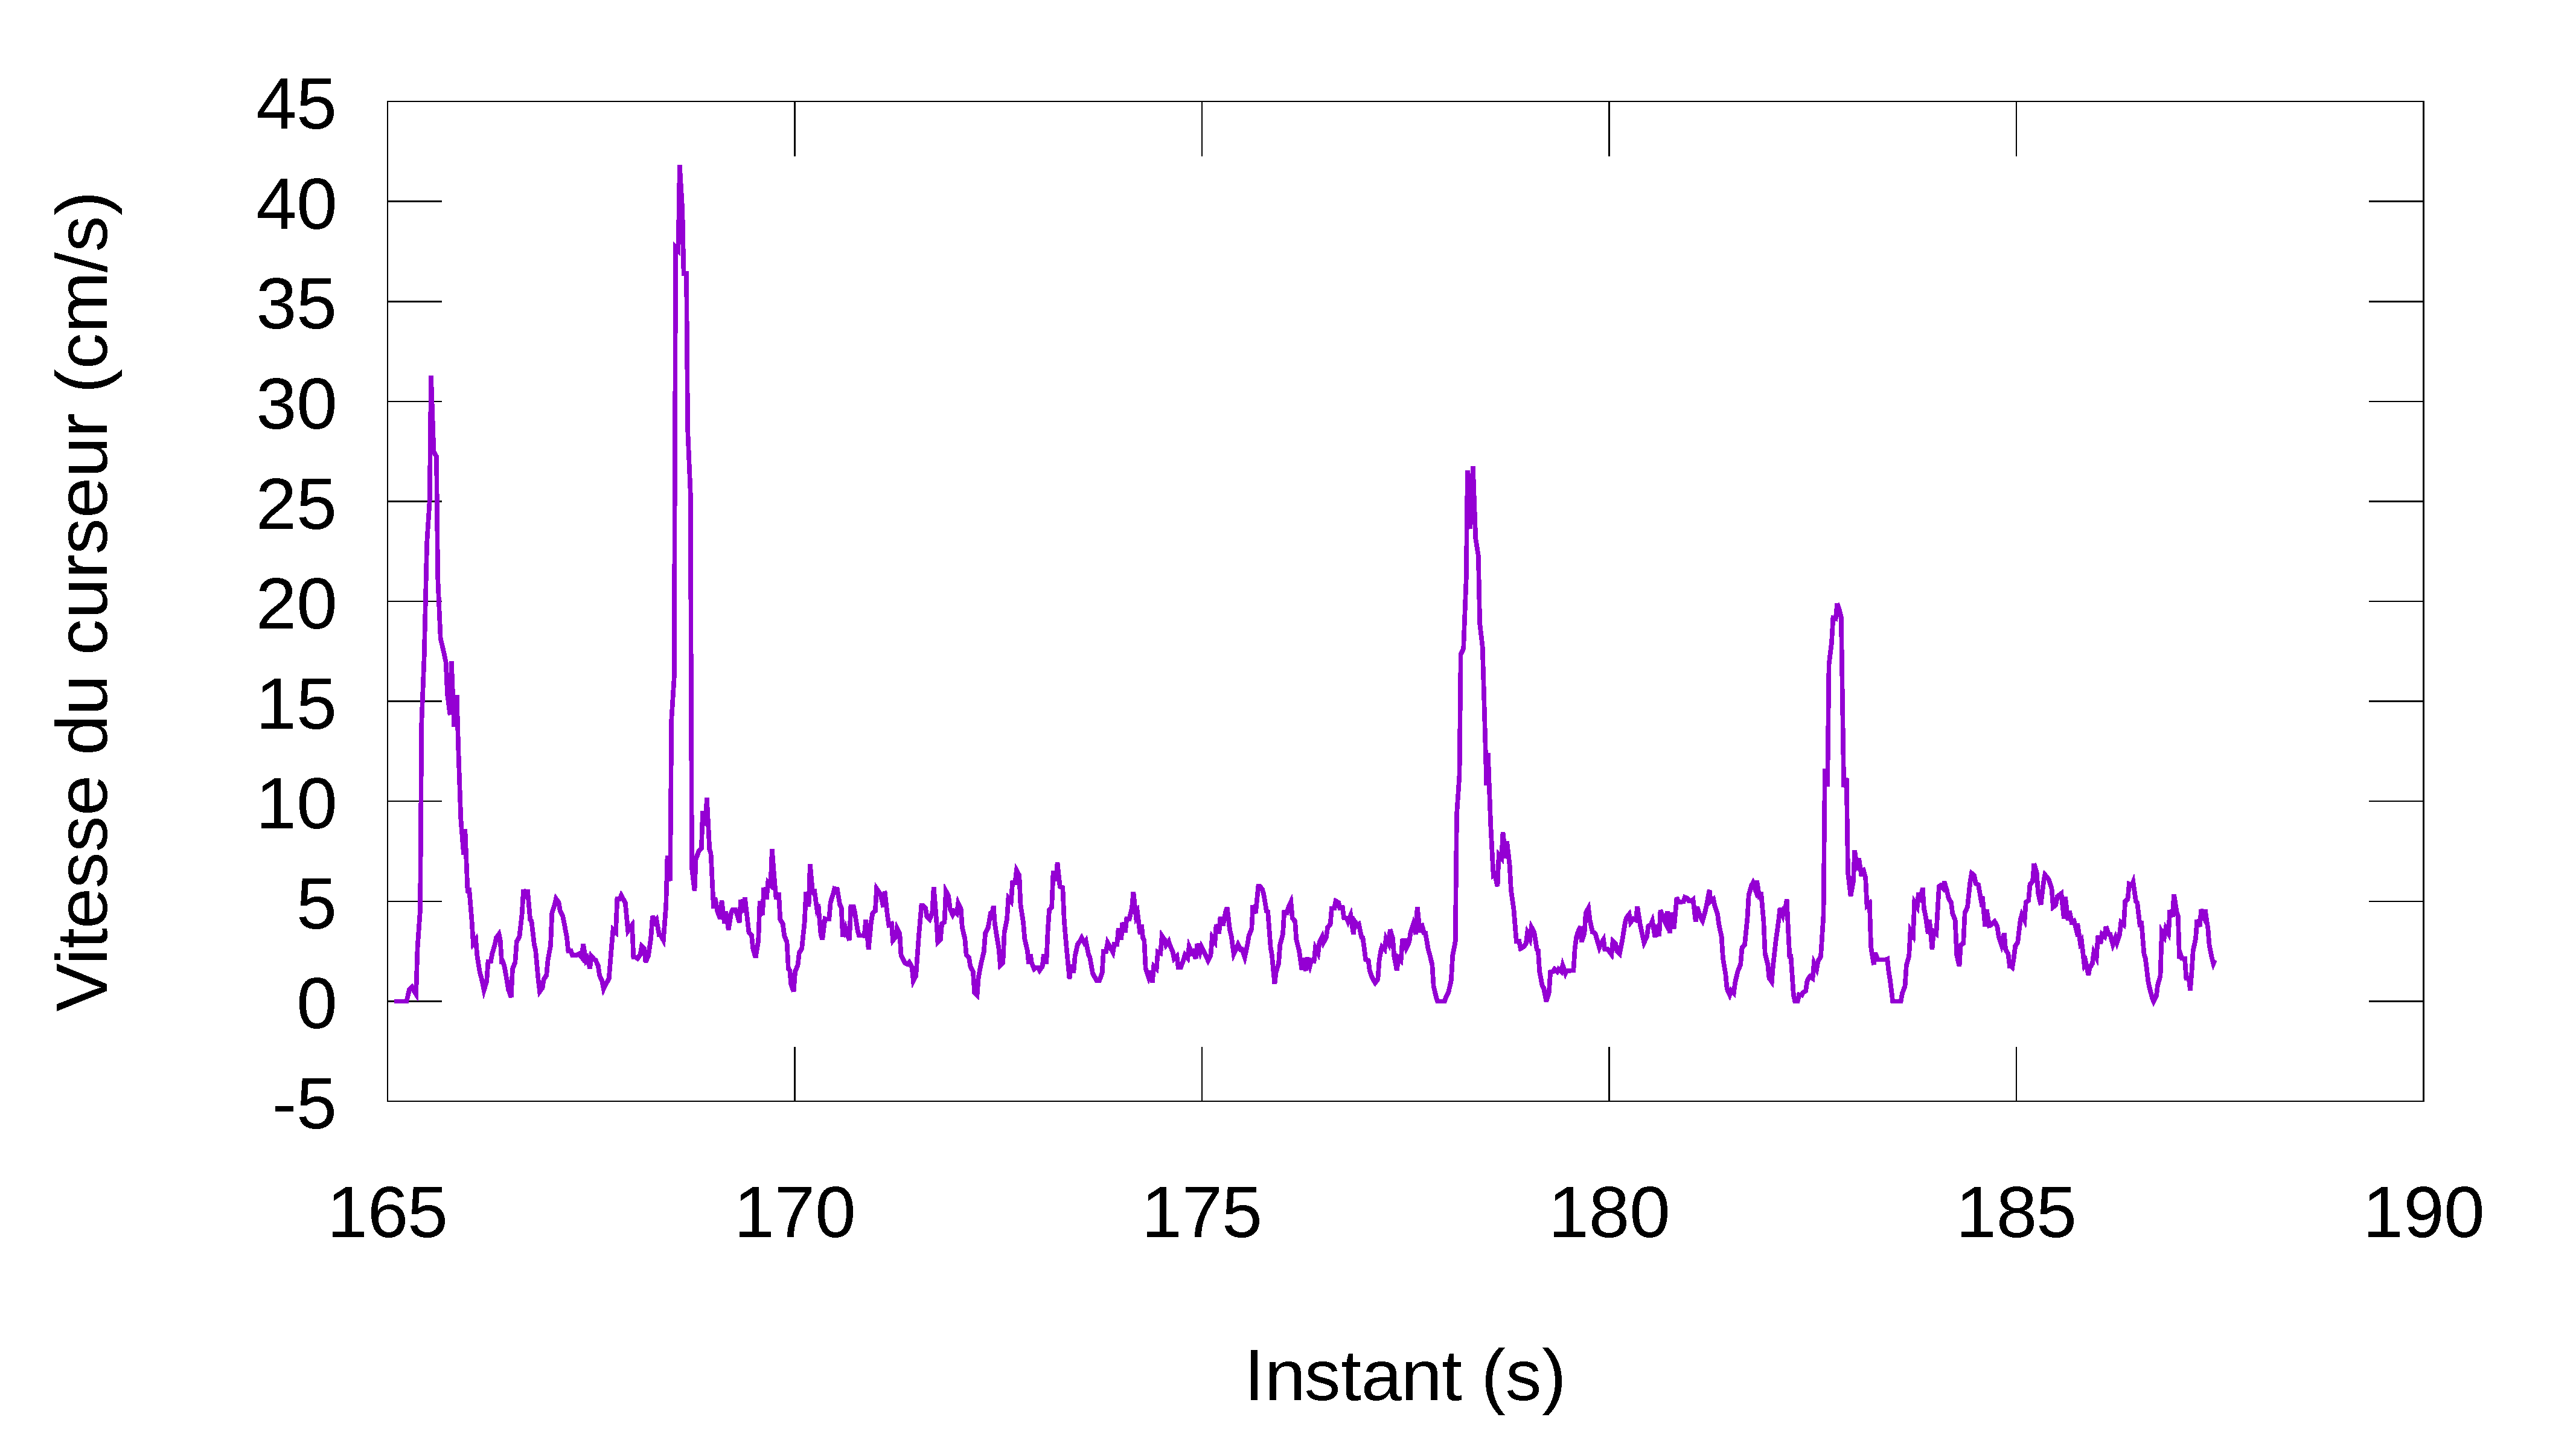
\includegraphics[width=\textwidth]{figures/ch4/subject_06_60_13_219_smoothed}
			\caption{Profil du sujet 6.}
			\label{fig:hardProfile6}
		\end{subfigure}
		~
		\begin{subfigure}[t]{\subImgWlineplot}
			\centering
			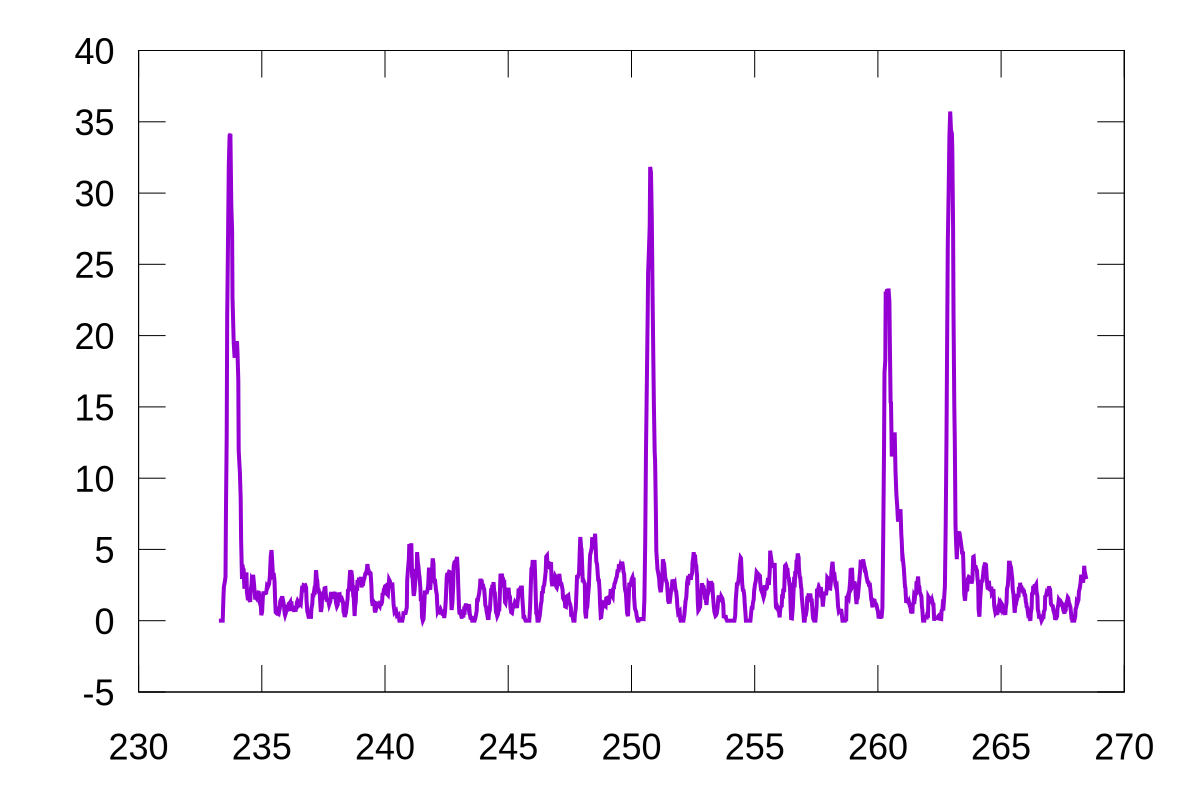
\includegraphics[width=\textwidth]{figures/ch4/subject_08_180_8_219_smoothed}
			\caption{Profil du sujet 8.}
			\label{fig:hardProfile8}
		\end{subfigure}
		~
		\begin{subfigure}[t]{\subImgWlineplot}
			\centering
			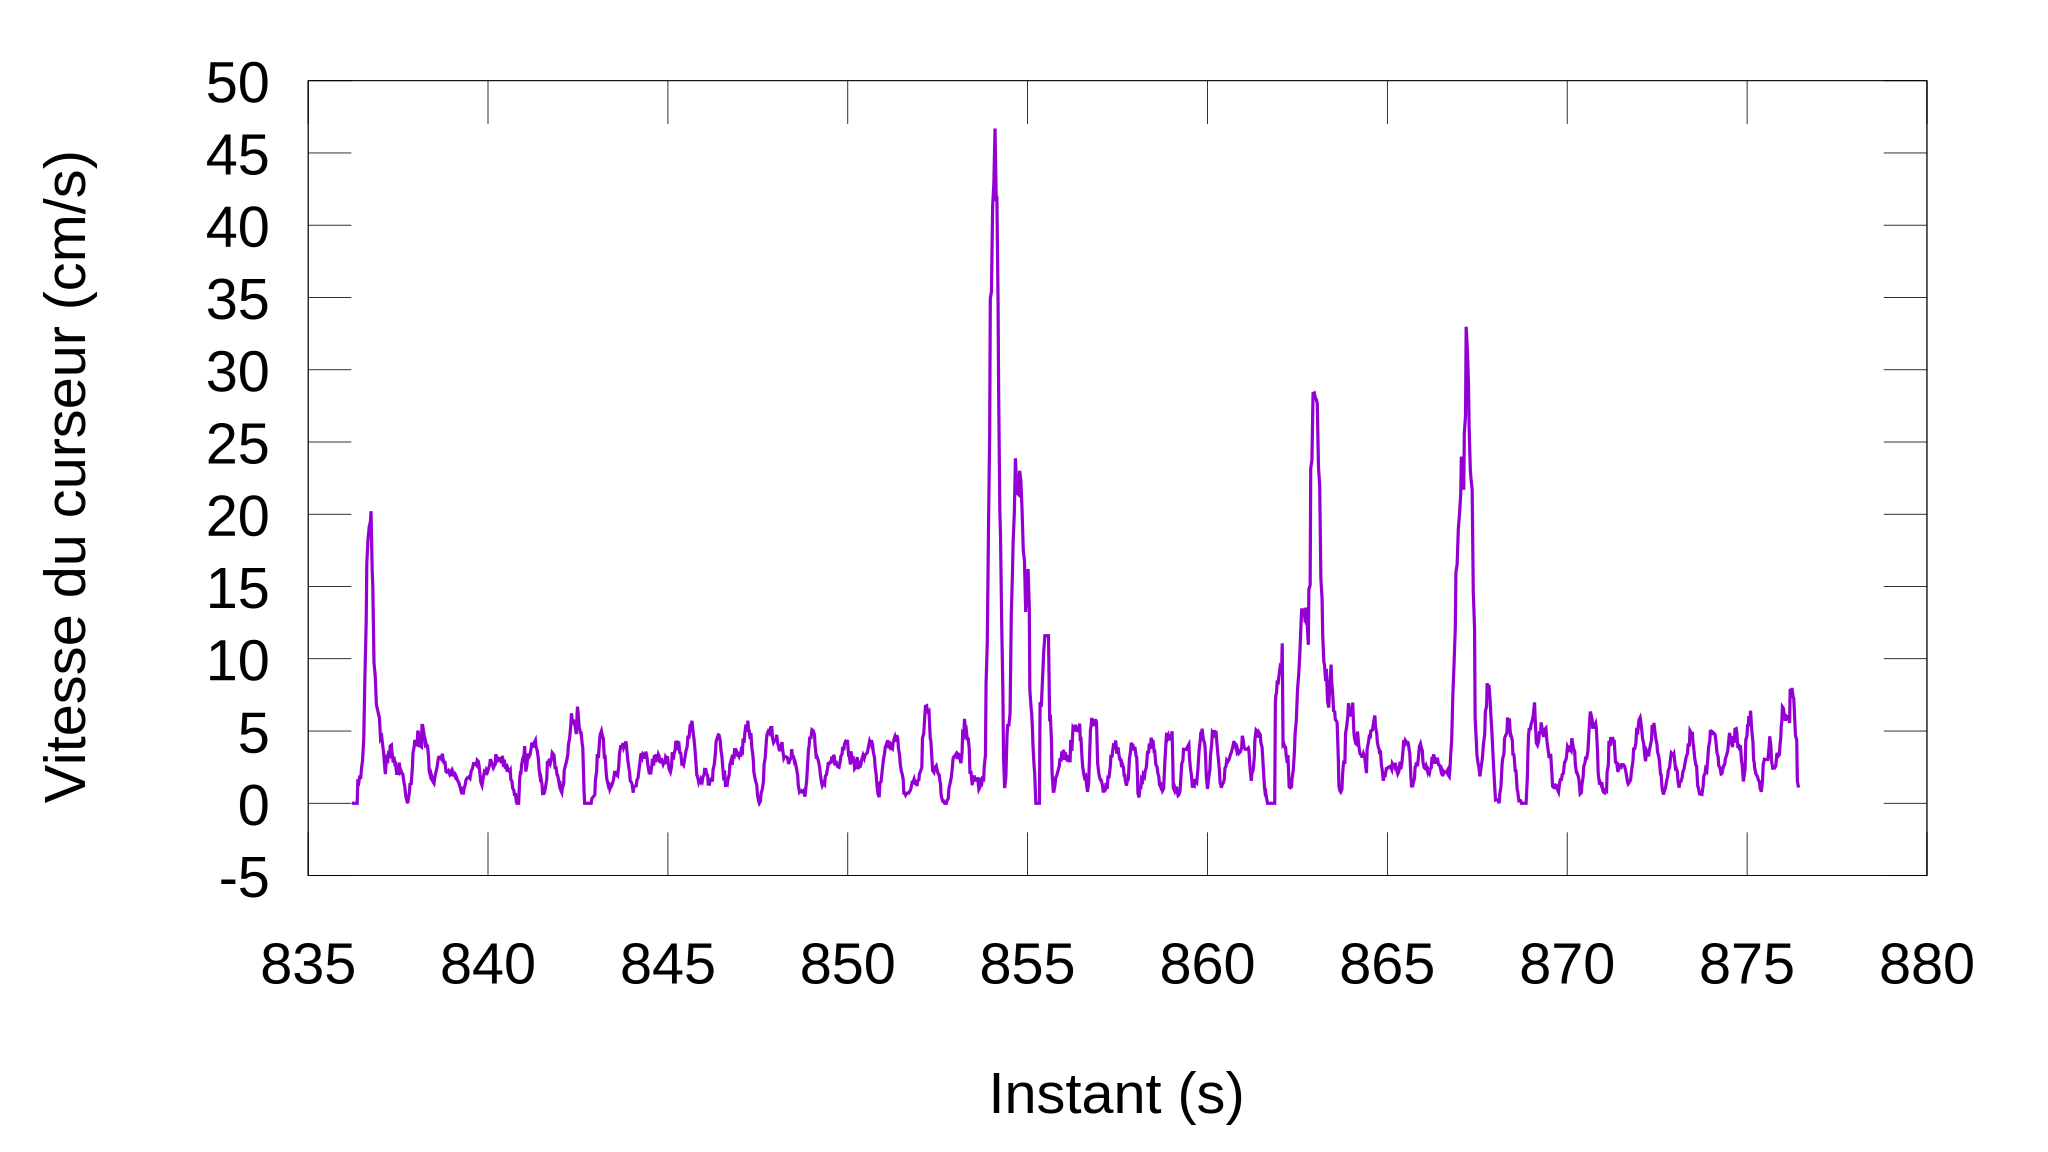
\includegraphics[width=\textwidth]{figures/ch4/subject_09_30_30_219_smoothed}
			\caption{Profil du sujet 9.}
			\label{fig:hardProfile9}
		\end{subfigure}
		\caption[Profils de vitesse du curseur, conditions]{Profils lissés de vitesse du curseur pour quatre sujets, avec des cibles de mouvements imprévisibles à 2,19~cm/s. Le temps (en secondes) est en abscisse et la vitesse (en cm/s) est en ordonnée. Nous avons ici sélectionné des profils correspondant à des conditions difficiles pour chaque sujet.}
		\label{fig:hardProfiles}
	\end{figure}
	
	Une représentation plus objective et quantitative de cette observation est proposée dans la table~\ref{tab:cursorSpeedTough}, où l'on observe les vitesses moyennes du curseur en fonction des sujets et des types de condition. Comme on le voit, les vitesses moyennes sont considérablement réduites pour les conditions difficiles, en dépit du fait que les vitesses maximales ne sont pas significativement différentes, comme l'illustrent les hauteurs des pics sur la figure~\ref{fig:hardProfiles}. Cette réduction de la vitesse moyenne est donc bien due au rallongement des phases de correction.
	
	\begin{table}
		\centering
		\begin{tabular}{c | c c c | c c}
					& \multicolumn{3}{c |}{Vitesses moyennes}		& \multicolumn{2}{c}{Différences de pourcentage}	\bigstrut[b] \\
			Sujet	& Statique		& Rectiligne	& Imprévisible	& Stat--impr.		& Rect-impr.					\bigstrut[b] \\ \hline
			5		& 11,10~cm/s	& 8,00~cm/s		& 5,89~cm/s		& 61,29~\%{}		& 30,36~\%{}					\bigstrut[t] \\
			6		& 9,82~cm/s		& 8,57~cm/s		& 4,41~cm/s		& 76,14~\%{}		& 64,20~\%{}					\\
			8		& 7,65~cm/s		& 7,05~cm/s		& 2,85~cm/s		& 91,33~\%{}		& 84,77~\%{}					\\
			9		& 8,48~cm/s		& 6,46~cm/s		& 4,14~cm/s		& 68,79~\%{}		& 43,85~\%{}					\\
		\end{tabular}
		\caption[Vitesses du curseur, cibles statiques, rectilignes ou imprévisibles]{Vitesses moyennes (en cm/s) du curseur pour quatre sujets différents, au cours de sélections de cibles statiques, en mouvement rectiligne, ou imprévisibles. Les différences de pourcentages entre les conditions sont présentées dans les deux dernières colonnes (\emph{stat-impr} pour les différences entre cibles statiques et de mouvements imprévisibles, \emph{rect-impr} pour les différences entre cibles de mouvement rectiligne et imprévisibles).}
		\label{tab:cursorSpeedTough}
	\end{table}
	
	\subsection{Prédominance de la phase de correction}
	Si, pour des cibles statiques, les phases balistique et de correction sont à peu près équilibrées dans le temps, comme l'illustre la figure~\ref{fig:staticProfiles}, la figure~\ref{fig:rectProfiles} montre que ce n'est plus vraiment le cas avec des cibles se déplaçant en ligne droite, et la figure~\ref{fig:hardProfiles} nous apprend que ce n'est plus du tout vrai lorsque les mouvements des cibles sont imprévisibles, la phase de correction dominant alors le temps total de sélection.
	
	Il est donc logique de recommander à qui souhaiterait concevoir une technique d'assistance à la sélection de cibles mobiles de concentrer ses efforts sur la réduction de la durée de la phase de correction, et ce d'autant plus que les mouvements des cibles des applications visées sont imprévisibles. En effet, la loi d'Amdahl~\cite{amdahl1967validity} nous permet de quantifier l'accélération possible d'une tâche hétérogène en fonction d'une part de la portion de la tâche qu'il est possible d'accélérer, et d'autre part du niveau d'accélération possible sur cette portion.
	
	Cette loi s'énonce formellement selon l'équation~\ref{eq:amdahl}, où $S(s)$ est l'accélération totale de la tâche (facteur sans unité), $p$ est la proportion (en temps) de la tâche qui peut être accélérée, et $s$ est l'accélération possible sur cette portion (facteur sans unité). Or, il est évident que cette loi implique la limite énoncée dans l'équation~\ref{eq:amdahlLimit}.
	
	\begin{align}
		\label{eq:amdahl}
		S(s) &= \frac{1}{(1-p) + \frac{1}{s}} \\
		\label{eq:amdahlLimit}
		\lim_{s\to\infty} S(s) &= \frac{1}{1-p}
	\end{align}
	
	Cette limite quand $s$ tend vers l'infini correspond à l'accélération maximale qu'il serait possible d'obtenir avec une technique d'assistance à la sélection \og parfaite \fg{}, c'est-à-dire réduisant le temps de sélection à zéro, mais seulement sur une partie de la tâche représentant une proportion $p$ de son temps de complétion. La figure~\ref{fig:amdahl} en fournit une représentation graphique. Comme on le constate, pour de petites valeurs de $p$, l'accélération maximale théoriquement possible reste faible, si bien qu'il nous paraît déraisonnable de concentrer ses efforts sur une phase de la tâche de sélection représentant moins de 30~\%{} du temps total de la tâche.
	
	\begin{figure}[!htb]
		\centering
		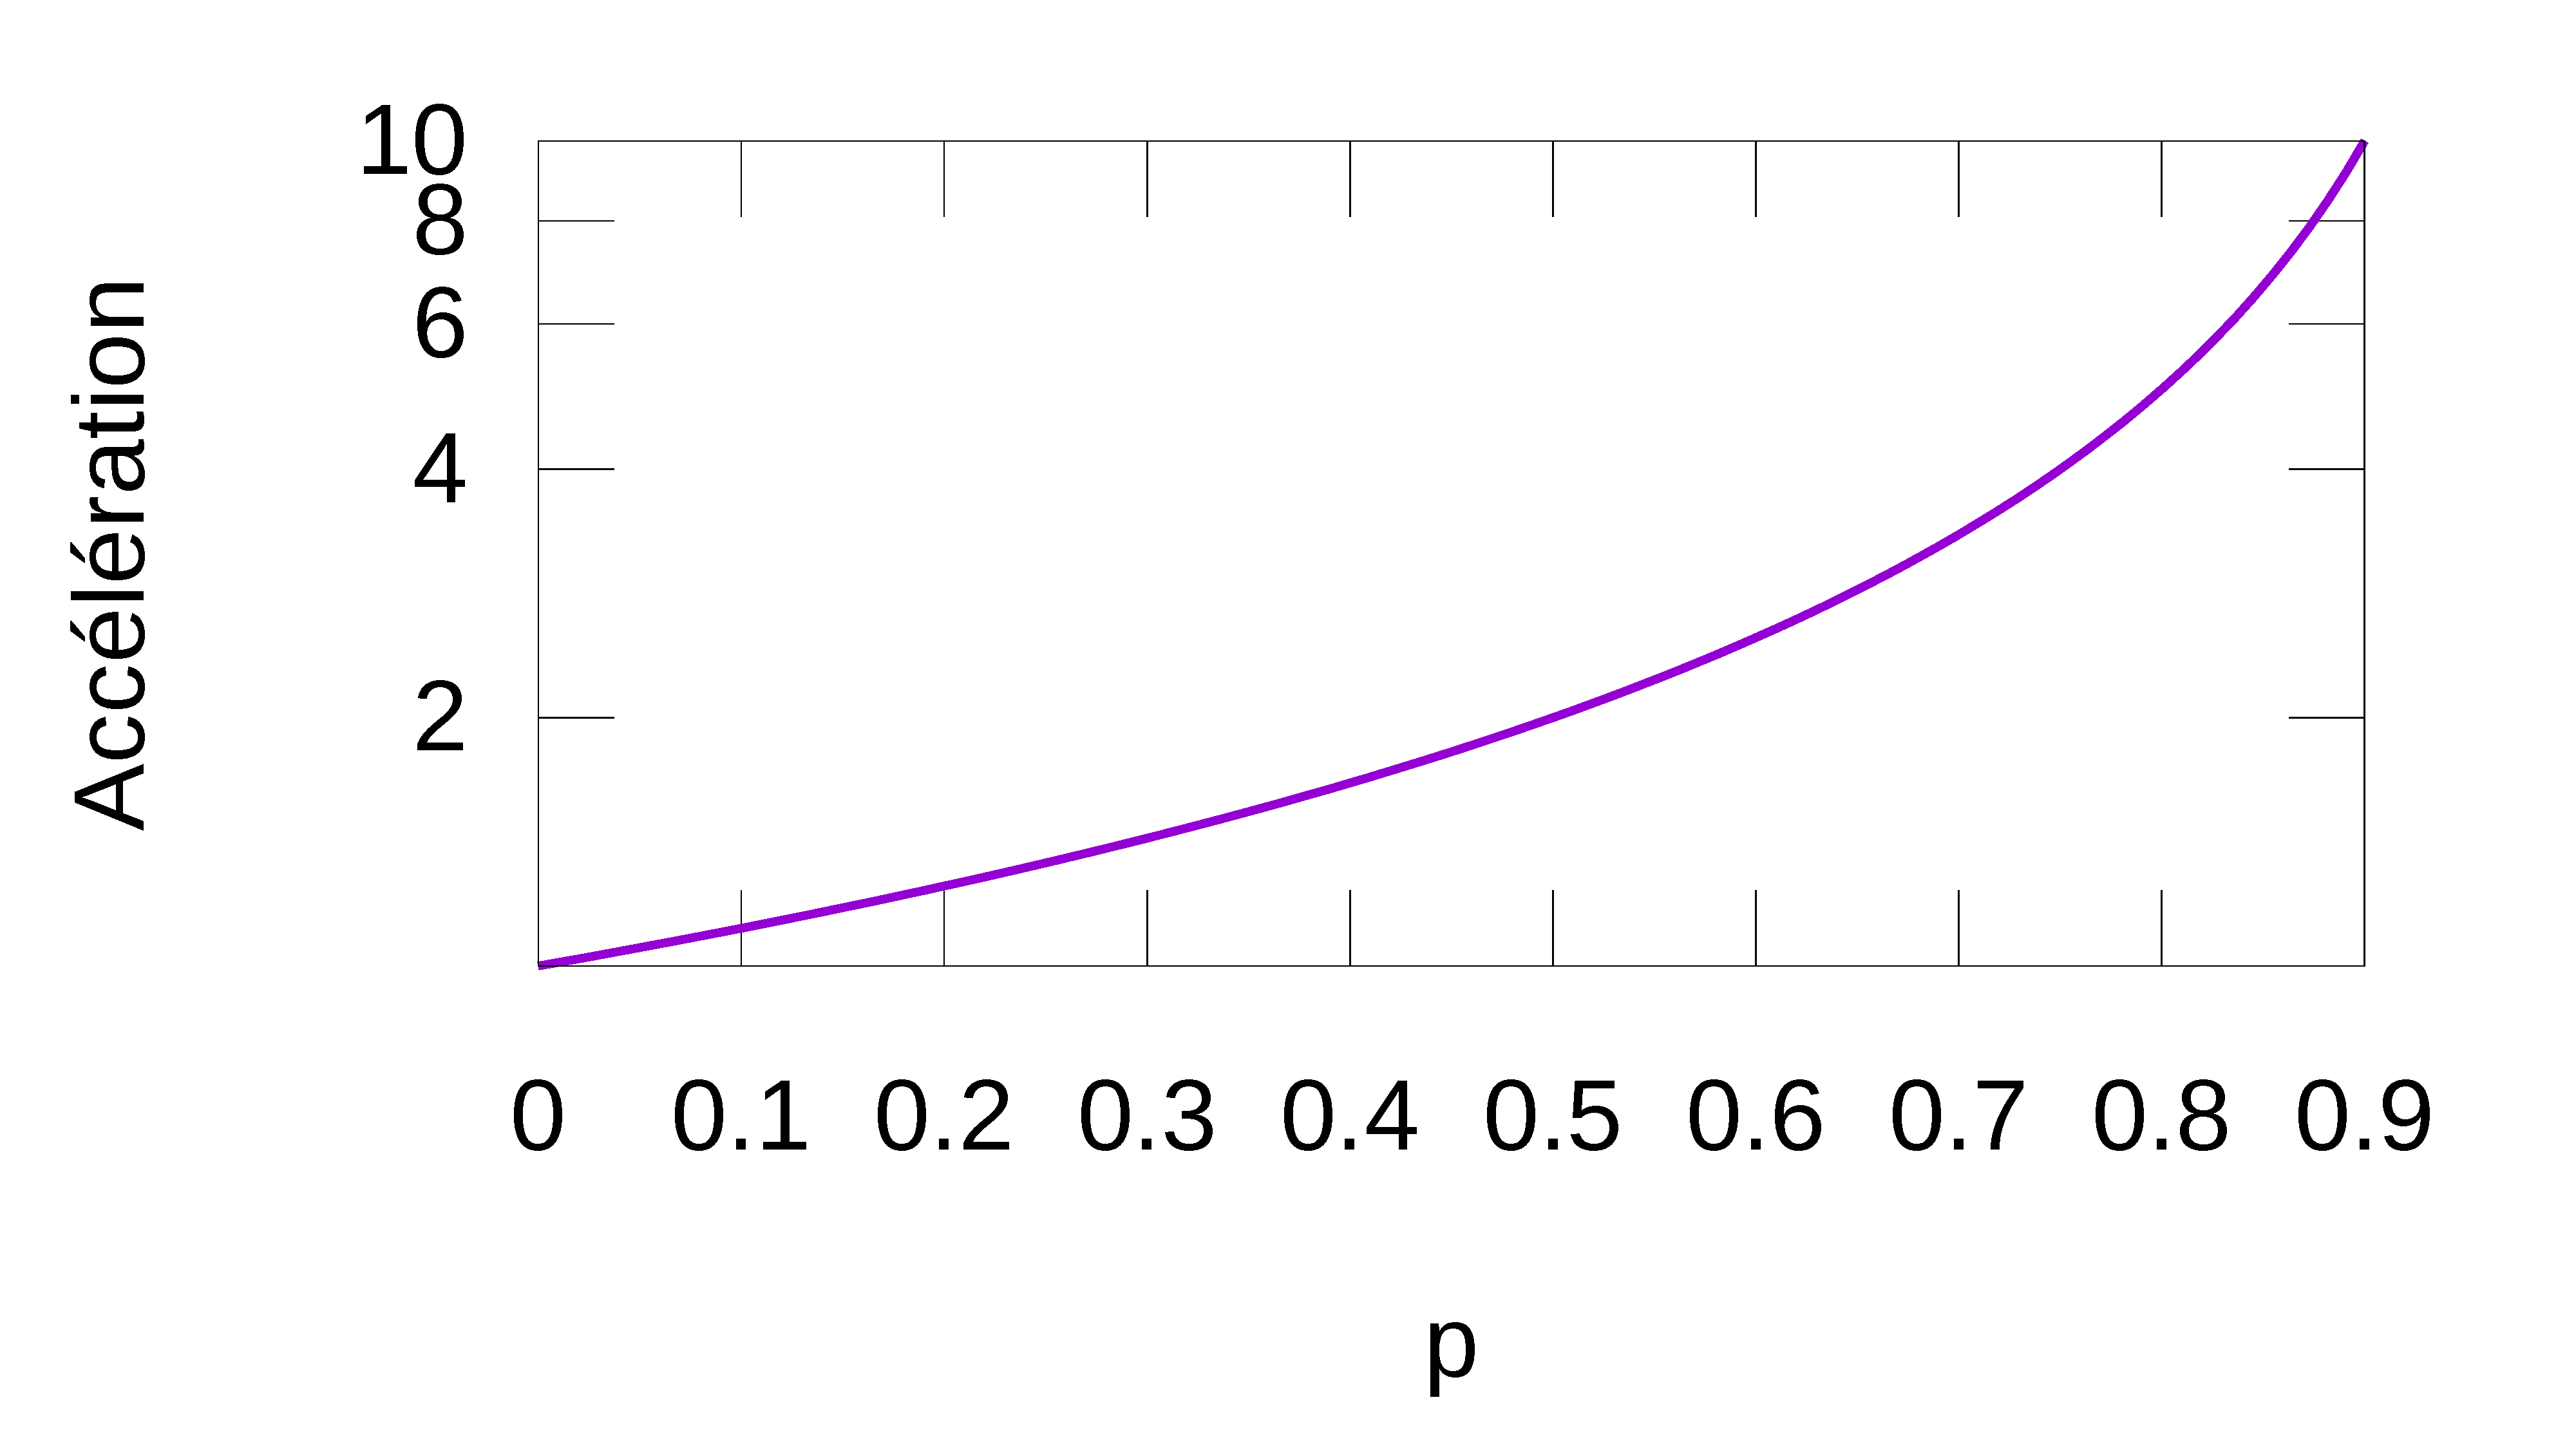
\includegraphics[width=\textwidth]{figures/ch4/amdahl}
		\caption[Loi d'Amdahl sous sa forme de limite]{Loi d'Amdahl sous sa forme de limite, quand le taux d'accélération de la sous-tâche tend vers l'infini. La courbe violette représente l'accélération maximale possible pour une tâche dont une sous-tâche représentant une proportion $p$ de son temps de complétion initial peut être accélérée à l'infini ; c'est-à-dire que le temps de complétion de cette sous-tâche peut être réduit à zéro. Cette fonction diverge en $p = 1$.}
		\label{fig:amdahl}
	\end{figure}
	
	La phase de correction étant en revanche susceptible de représenter une très grande portion du temps de sélection (cela peut dépasser les 80~\%{} pour les conditions les plus difficiles) l'on voit bien que les gains potentiels sont considérables, si l'on parvient à obtenir une accélération $s$ importante sur cette phase. Une technique d'assistance à la sélection de cibles mobiles devrait donc se focaliser sur cette phase.
	
\section{Aires des enveloppes convexes et temps de sélection}
	Pour rappel, l'enveloppe convexe d'un ensemble de points du plan est le plus petit polygone convexe contenant tous les points de l'ensemble. Nous montrions dans le chapitre~\ref{chap3} (en particulier sur la figure~\ref{fig:spEffect}) que l'aire de l'enveloppe convexe d'une trajectoire générée par notre modèle VFA dépendait fortement de la vitesse.
	
	\subsection{L'aire : une fonction linéaire de la vitesse}
	Si l'on considère une cible comme un object ponctuel --- donc d'aire nulle --- il est évident que si $V = 0$, la cible ne bougera pas et l'aire de son enveloppe convexe sera nulle. Dès lors, l'on peut formuler l'hypothèse que l'aire de l'enveloppe convexe d'une trajectoire générée par le modèle VFA est une fonction linéaire de la vitesse, c'est-à-dire que $\mathcal{A}(ec) = \gamma{}V$ où $\mathcal{A}(ec)$ est l'aire de l'enveloppe convexe $ec$, et $\gamma \in \mathbb{R}$.
	
	Nous avons évalué cette hypothèse en fixant les valeurs de A et F, et en faisant varier V pour mesurer l'impact sur $\mathcal{A}(ec)$. La figure~\ref{fig:avspeed} fournit une illustration de telles mesures, en l'occurrence avec $A = 120\degree$ et $F = 8$~Hz. Toutes nos mesures avec d'autres valeurs de A et F sont cohérentes. Notez que les aires utilisées pour ce graphique, correspondent à l'aire moyenne sur 400 trajectoires générées aléatoirement pour chaque valeur de V.
	
	\begin{figure}[!htb]
		\centering
		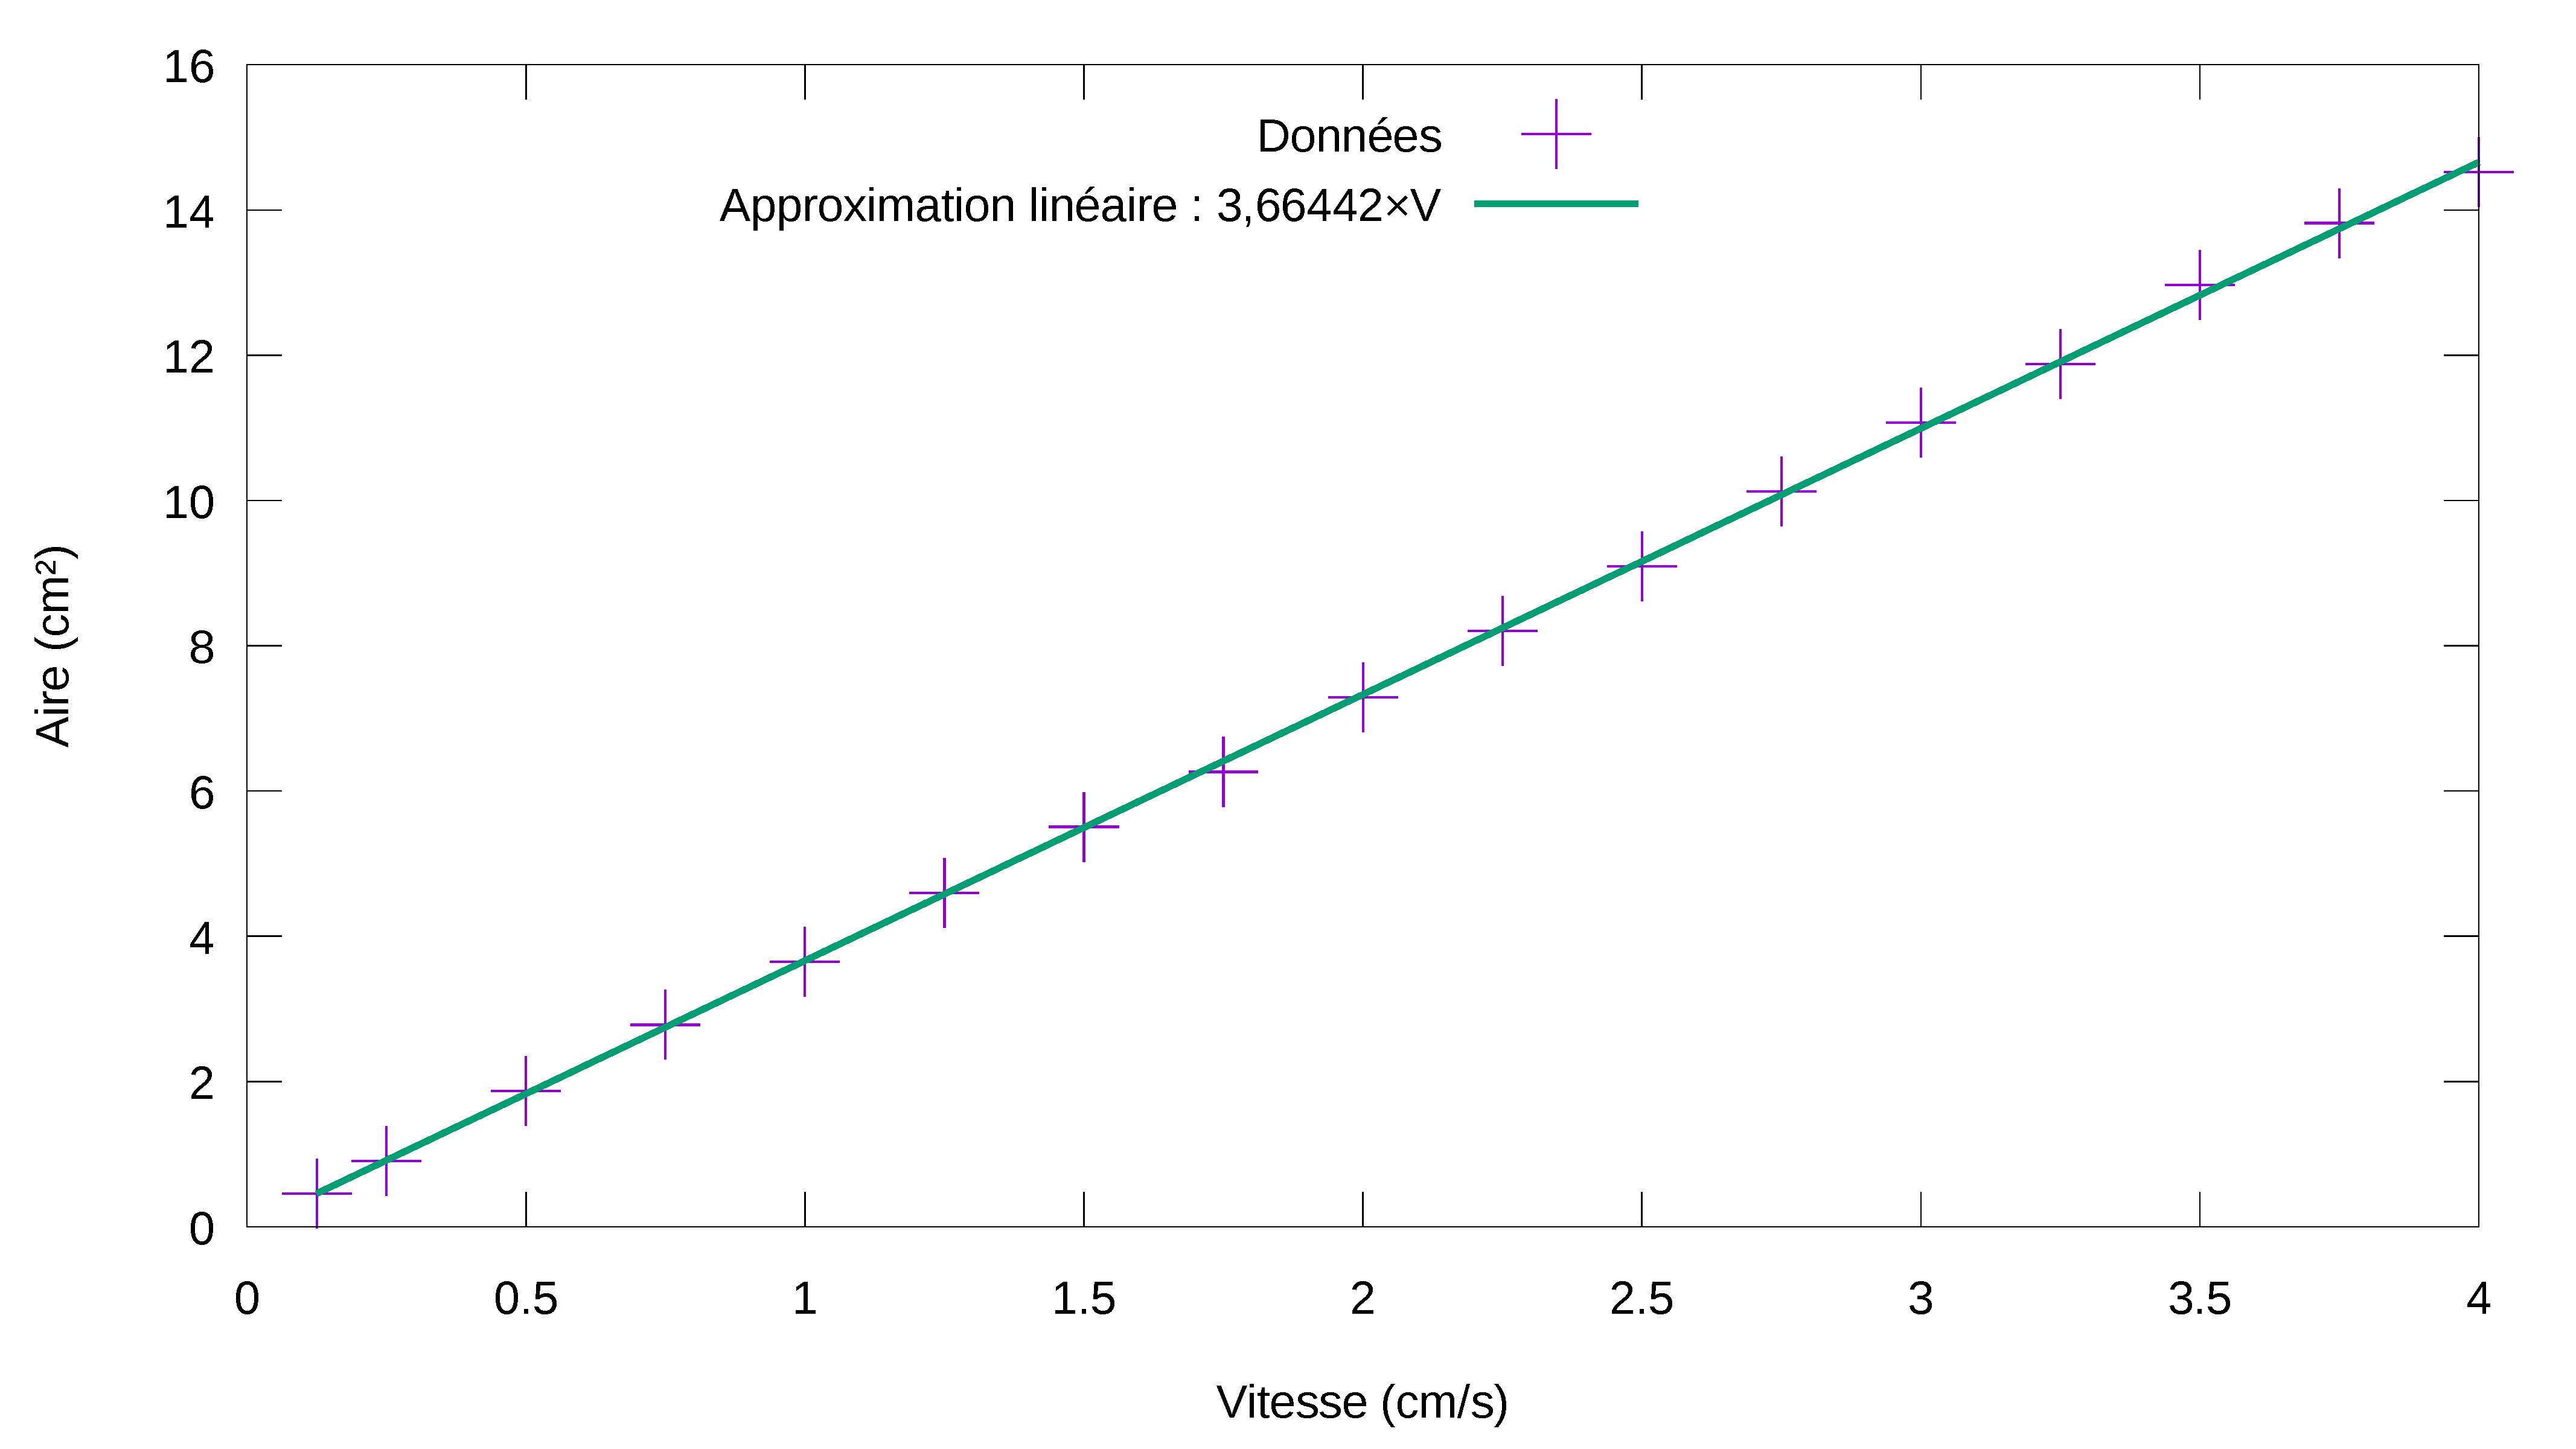
\includegraphics[width=\textwidth]{figures/ch4/areaVspeed}
		\caption[Aire de l'enveloppe convexe en fonction de la vitesse]{Aire de l'enveloppe convexe d'une trajectoire (de 5 secondes) en fonction de la vitesse. Les paramètres A et F sont fixés (à respectivement 120\textdegree{} et 8~Hz) et la vitesse varie de 0,125~cm/s à 4~cm/s. Pour chaque valeur de V, on mesure l'aire moyenne de l'enveloppe convexe de la trajectoire génrée. Les mesures sont en bleu et une approximation linéaire est représentée en rouge, avec son équation et son coefficient de détermination $R^{2} > 0,9999$.}
		\label{fig:avspeed}
	\end{figure}
	
	\subsection{Détermination des coefficients}
	Cependant, si l'on a bien $\mathcal{A}(ec) = \gamma{}V$, $\forall A$ et $\forall F$, la valeur de $\gamma$ n'est pas la même pour toutes les combinaisons de A et F. De fait, la vitesse ne peut être tenue pour totalement indépendante des autres paramètres. Nous avons donc cherché à déterminer la valeur de $\gamma$ en fonction de F et A, de manière à pouvoir étudier $\mathcal{A}(ec)$ en fonction de F et A.
	
	Pour ce faire, nous avons généré des trajectoires pour diverses combinaisons de F et A à de nombreuses valeurs de V, afin de déterminer la valeur de $\gamma$ correspondant à chaque couple (F,A). Encore une fois, pour chaque condition (V,F,A) nous avons généré de multiples trajectoires (100), afin d'obtenir des valeurs moyennes fiables. Les résultats sont présentés sous forme de cartes thermiques sur la figure~\ref{fig:gammaVfa}. La figure~\ref{fig:gammaVfaLin} les représente avec F sur une échelle linéaire, et la figure~\ref{fig:gammaVfaLog} avec F sur une échelle logarithmique, pour plus de lisibilité.	
	
	\begin{figure}[!htb]
		\centering
		\begin{subfigure}[t]{\textwidth}
			\centering
			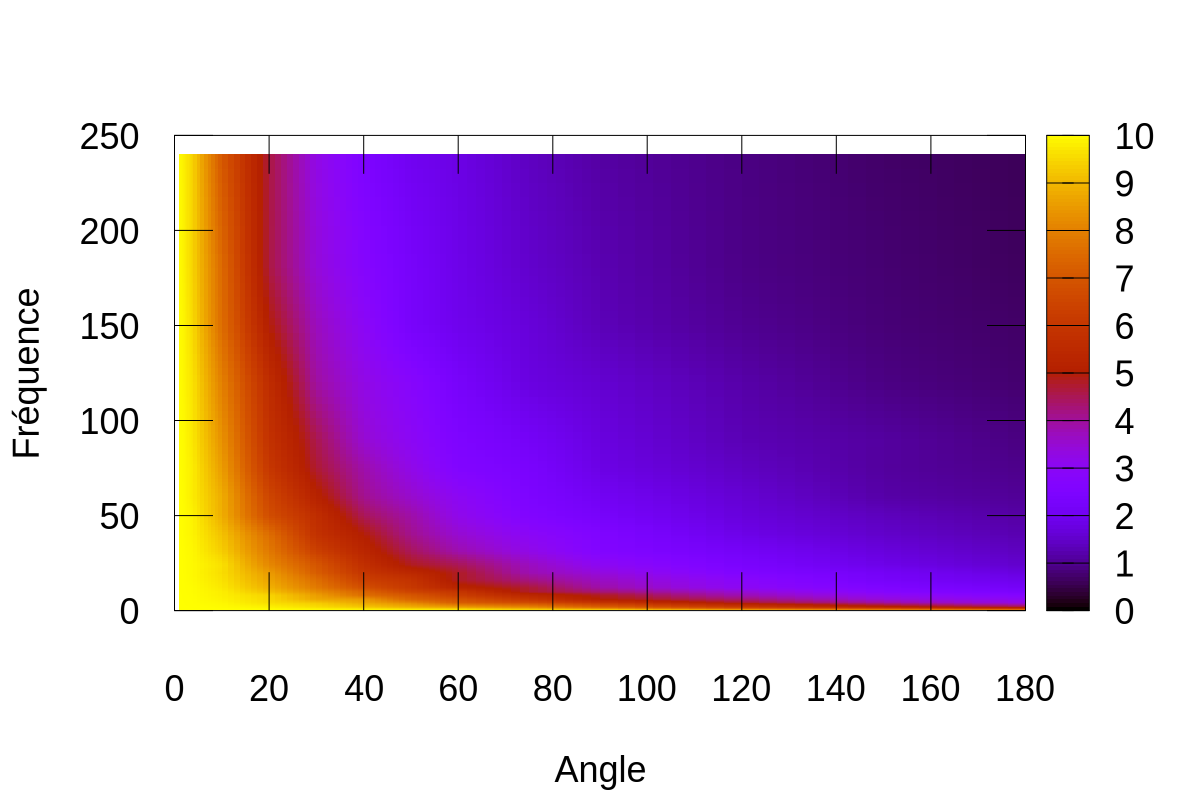
\includegraphics[width=\textwidth]{figures/ch4/linApprox}
			\caption{Échelle linéaire.}
			\label{fig:gammaVfaLin}
		\end{subfigure}
		~
		\begin{subfigure}[t]{\textwidth}
			\centering
			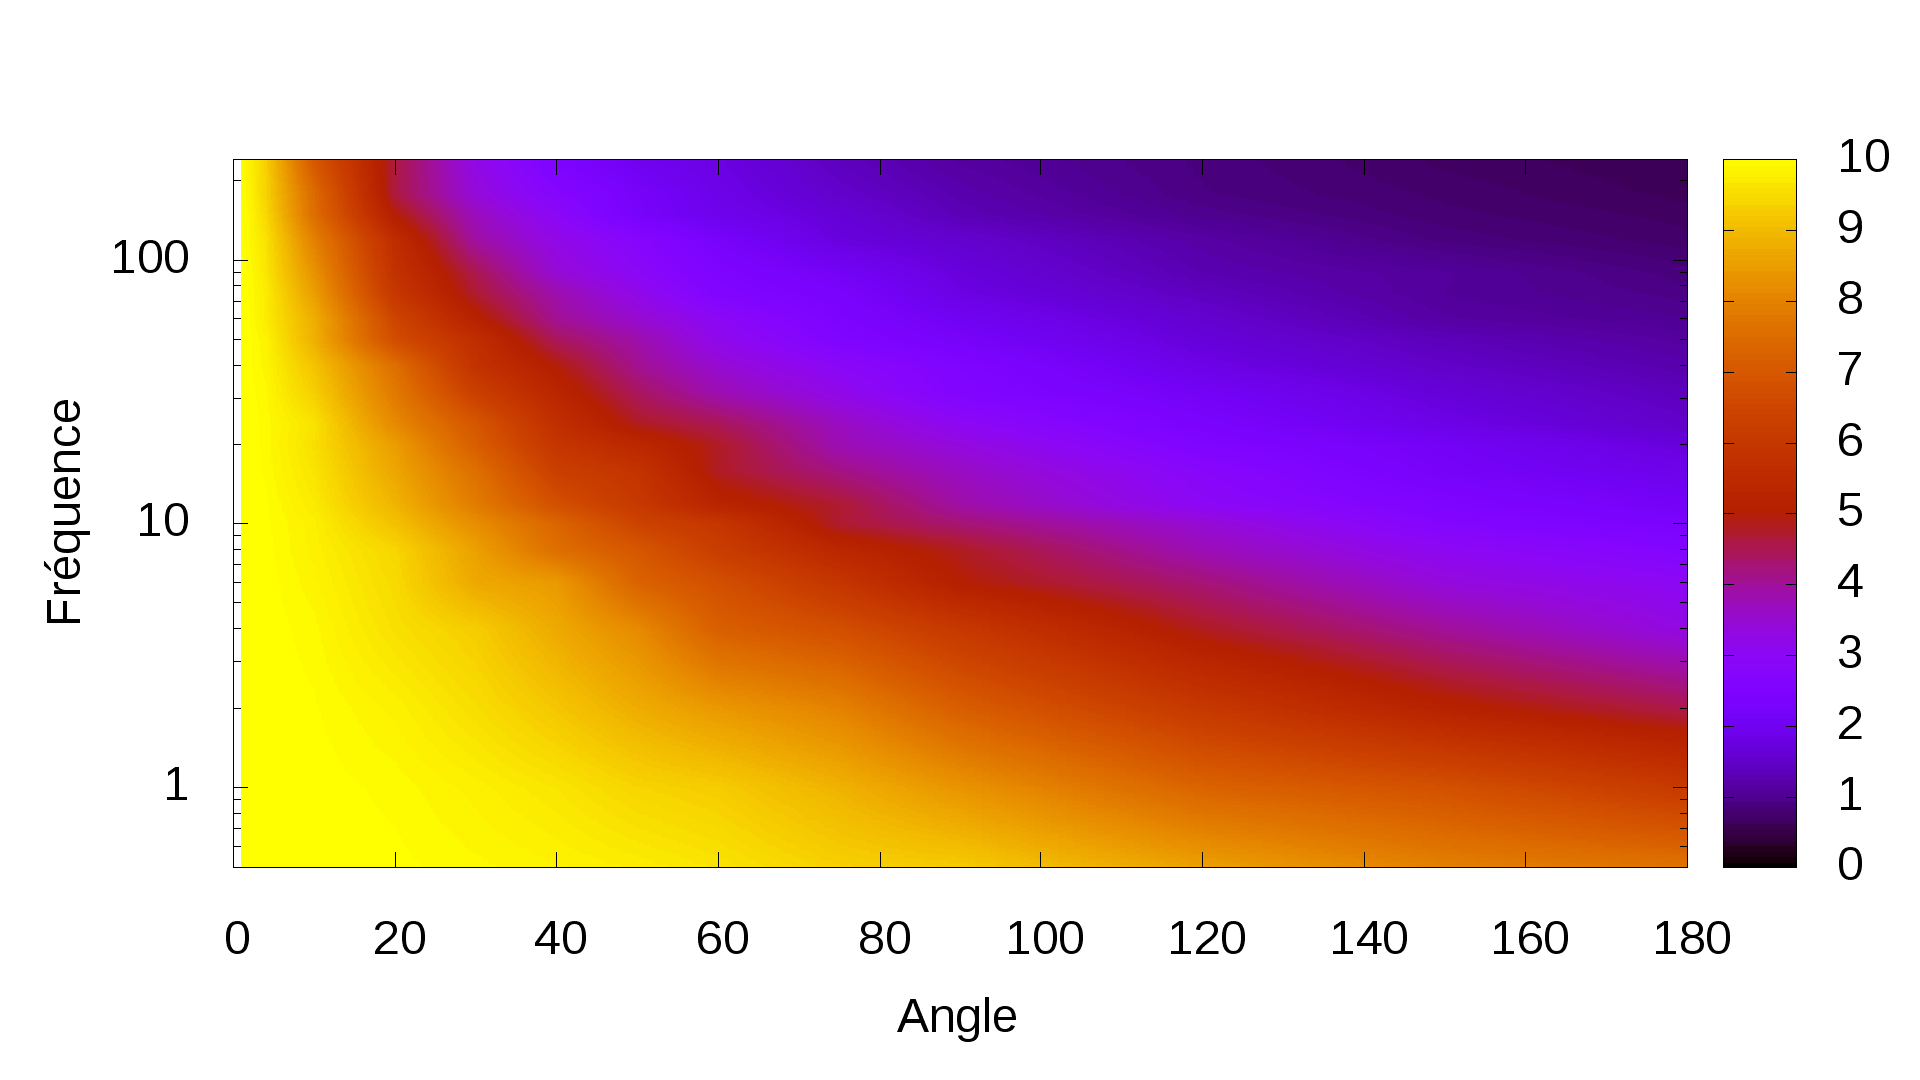
\includegraphics[width=\textwidth]{figures/ch4/linApprox_log}
			\caption{Échelle logarithmique.}
			\label{fig:gammaVfaLog}
		\end{subfigure}
		\caption[Coefficients $\gamma$ en fonction de F et A]{Coefficients $\gamma$ en fonction de F et A. La fréquence se lit en ordonnée, le paramètre d'angle en abscisse, et la valeur de $\gamma$ est indiquée par la couleur ; elle est comprise entre 0 et 10.}
		\label{fig:gammaVfa}
	\end{figure}
	
	Ces données nous fournissent un moyen d'obtenir, à partir d'une aire de référence pour un couple (F,A), l'aire réelle en fonction de V, simplement en multipliant l'aire de référence par $\gamma{}V$. Si le couple (F,A) en question n'est pas présent dans les données brutes ayant permis de générer la figure~\ref{fig:gammaVfa}, la continuité de la fonction qui à un couple (F,A) associe une valeur de $\gamma$ nous autorise à approximer la valeur recherchée à l'aide d'une simple interpolation bilinéaire. Il serait bien entendu possible de calculer une grille de référence plus fine et plus précise.
	
	\subsection{Pseudo-entropie et valeur de $\gamma$}
	Si la figure~\ref{fig:gammaVfaLin} suggère que l'augmentation de A et de F ont le même effet sur $\gamma$, à savoir en diminuer la valeur, la figure~\ref{fig:gammaVfaLog} montre que, dès lors que A atteint une valeur relativement élevée (autour de 50) la fréquence a un impact très important sur la valeur de $\gamma$. L'inverse est moins vrai : même à de très hautes fréquences, l'impact du paramètre d'angle n'est pas si fort.
	
	On peut donc supposer que le produit AF ne serait pas un très bon prédicteur de $\gamma$, car le poids de F serait trop fort\ldots{} Mais une expression de la forme $A\times{}F^{k}$ avec $k \in [0,1]$ pourrait être plus appropriée. Des essais empiriques avec différentes valeurs de $k$ montrent que la meilleure est $k = \frac{1}{2}$, c'est-à-dire l'expression $A\sqrt{F}$. La figure~\ref{fig:gammaAF} confirme, par la multiplicité des valeurs de $\gamma$ dans un petit intervalle de valeurs de AF, que ce n'est pas la bonne façon d'exprimer ce coefficient en fonction des paramètres du modèle VFA ; la figure~\ref{fig:gammaASQRTF} illustre la pertinence de la forme $A\sqrt{F}$.

	\begin{figure}[!htb]
		\centering
		\begin{subfigure}[t]{\textwidth}
			\centering
			\includegraphics[width=\textwidth]{figures/ch4/afVgamma}
			\caption{$\gamma$ en fonction de $A\times{}F$.}
			\label{fig:gammaAF}
		\end{subfigure}
		~
		\begin{subfigure}[t]{\textwidth}
			\centering
			\includegraphics[width=\textwidth]{figures/ch4/asqrtFVgamma}
			\caption{$\gamma$ en fonction de $A\sqrt{F}$.}
			\label{fig:gammaASQRTF}
		\end{subfigure}
		\caption[Coefficients $\gamma$ en fonction de F et A, bis]{Coefficients $\gamma$ en fonction de F et A. Les valeurs de $\gamma$ sont en ordonnée, et l'expression contenant A et F est en abscisse. On remarque que la seconde expression fondée sur la racine carrée de F correspond bien mieux aux valeurs de $\gamma$.}
		\label{fig:gammaVentropy}
	\end{figure}
	
	Il est donc possible, à partir du produit $A\sqrt{F}$, de se passer de l'étape d'interpolation bilinéaire pour estimer la valeur de $\gamma$ : il suffit de calculer le produit $A\sqrt{F}$ et de le comparer aux valeurs de référence, éventuellement avec une simple interpolation linéaire. L'ajustement d'une fonction à la courbe de la figure~\ref{fig:gammaASQRTF} fournirait une solution encore plus simple.

%\section{Conclusion and perspectives}
%We have proposed a way to characterize the erratic behavior of moving targets with three parameters: speed, angle width and frequency, and tested pointing performance when varying these parameters. We have shown that the nature of target motion affects pointing performance, which is not captured by Fitts’ law’s index of difficulty. The latter can only describe the best case, and does not indicate that acquiring fast, highly erratic targets can be extremely difficult. Although the (S,A,F) set of parameters we have proposed models a continuum of target motion, our participants were able to distinguish at least three distinct categories that we have characterized (steady, vibrating and jerky). Our results suggest that for erratic targets, predictability determines pointing performance. And while the steady and vibrating categories are relatively predictable, the jerky one is not. We have also observed that the A×F product might be a promising way to assess predictability, although we still need more data to deduce a predictive law for the acquisition of erratic targets. Nevertheless, this preliminary work is a first step toward a more formal study of the acquisition of erratic targets, and introduces a way to better characterize or even control their movement. Ultimately, such a model could be instrumental in the design of new selection techniques.

\clearpage
